\documentclass[10pt,twocolumn]{article}

% ── Layout ───────────────────────────────────────────────────────────────────
\usepackage[margin=0.85in,columnsep=0.24in]{geometry}
\usepackage[T1]{fontenc}
\usepackage[utf8]{inputenc}
\usepackage{microtype}
\usepackage{newtxtext,newtxmath}
\usepackage{abstract}
\usepackage{dblfloatfix}
\usepackage[font=small,labelfont=bf]{caption}

% ── Core packages ────────────────────────────────────────────────────────────
\usepackage{amsmath}
\usepackage{mathtools}
\usepackage{bm}
\usepackage{graphicx}
\usepackage{booktabs}
\usepackage{multirow}
\usepackage{array}
\usepackage{xcolor}
\usepackage{tikz}
\usetikzlibrary{arrows.meta,positioning,fit,backgrounds,shapes.geometric,calc}
\usepackage[authoryear,round]{natbib}
\usepackage[colorlinks=true,linkcolor=blue,citecolor=blue,urlcolor=blue]{hyperref}
\usepackage{xurl}   % allow line breaks inside long bibliography URLs

\usepackage{colortbl}   % \cellcolor for the taxonomy table
\definecolor{goodgreen}{HTML}{2ECC71}
\definecolor{badred}{HTML}{E74C3C}

\renewcommand{\figurename}{Figure}
\renewcommand{\tablename}{Table}
\renewcommand{\abstractnamefont}{\normalfont\large\bfseries}
\renewcommand{\abstracttextfont}{\normalfont\small}
\setlength{\absleftindent}{0.35in}
\setlength{\absrightindent}{0.35in}
\setlength{\abovecaptionskip}{6pt}
\setlength{\belowcaptionskip}{2pt}
\setlength{\parindent}{1em}
\setlength{\parskip}{0pt}

% ── Theorem environments ─────────────────────────────────────────────────────
\newtheorem{definition}{Definition}

% ── Hyphenation hints for long technical terms ───────────────────────────────
\hyphenation{know-ledge-graph KG-RAG van-il-la sub-graph per-tur-ba-tion
             cal-i-bra-tion un-cer-tain-ty over-con-fi-dence semi-su-per-vised
             en-tro-py re-trieval}
\emergencystretch=2em

% ── Math shorthands ──────────────────────────────────────────────────────────
\newcommand{\R}{\mathbb{R}}
\newcommand{\E}{\mathbb{E}}
\newcommand{\cG}{\mathcal{G}}
\newcommand{\cE}{\mathcal{E}}
\newcommand{\cC}{\mathcal{C}}
\newcommand{\system}{OntoGraphRAG}
\DeclareMathOperator{\AUROC}{AUROC}
\DeclareMathOperator{\AUREC}{AUREC}

% ── Title ────────────────────────────────────────────────────────────────────
\title{When Answer Agreement Fails:\\
Retrieval-State Lock-In in Retrieval-Augmented Generation}
\author{\large Sahib Julka\\[0.25em]
\normalsize LMU University Hospital, LMU Munich\\
\normalsize \texttt{sahib.julka@med.lmu.de}}
\date{}

\begin{document}

\twocolumn[
\maketitle
\begin{onecolabstract}
Many black-box uncertainty methods used with retrieval-augmented generation
(RAG) read agreement among sampled answers as confidence.
That reasoning fails under \textbf{retrieval-state lock-in}: repeated samples see
the same defective retrieval state, empty or wrong, and the answer settles around
the error.
To diagnose the failure, the analysis separates three objects that a single
confidence score conflates: answer-state uncertainty (variation across sampled answers),
evidence-state uncertainty (whether retrieved passages support the answer), and
retrieval-state diagnostics (whether the graph retrieval state supplies
answer-relevant support).
Across six question-answering (QA) snapshots in an ontology-guided
knowledge-graph RAG (KG-RAG) system, answer-level uncertainty misses many
errors even under the deployable policies: at the operational five-sample
budget ($N=5$), $42\%$ of KG-RAG and $59\%$ of dense-retrieval errors show zero answer
dispersion.
The collapse is sharpest in a strict graph-only stress test (a mechanism probe,
not a deployment policy or one-component ablation); there, an answer-dispersion
score ranks clinical errors worse than chance (AUROC $0.233$).
A route decomposition splits the silent mass into an empty retrieval state
(\emph{absence}) and wrong-but-coherent neighbourhoods on bridge questions
(\emph{presence}); the latter remains open.
The recommendation follows directly: report the three families separately, and
treat an answer as low-risk only when all three agree, a conjunctive audit
rule that selects a small, high-precision subset. The rule is strongest on the
clinical calibration domain and weaker on open-domain multi-hop QA.
The point is diagnostic, not a claim that KG-RAG is more accurate than dense
retrieval: confidence in RAG is object-specific, and exposing the retrieval
state makes some confidence failures easier to diagnose.
\end{onecolabstract}
\vspace{1.0em}
]

\section{Introduction}
\label{sec:introduction}

Whether a RAG system can be trusted depends on more than the generated answer.
Retrieval relevance, evidence support, and usable provenance all matter
\citep{sun2024trustllm,ni2025trustworthyrag}.
Yet many black-box uncertainty estimators used with RAG still begin at the
answer surface.
Semantic entropy \citep{farquhar2024detecting,kuhn2023semantic},
SelfCheckGPT \citep{manakul2023selfcheckgpt}, and their RAG-integrated
variants \citep{jiang2023active,su2024dragin,zimmerman2024twotieredrag} ask,
in different forms, whether sampled answers agree.
Agreement is then used as a confidence signal, disagreement as uncertainty.
That assumption fails when retrieval repeatedly concentrates on the same
defective state. The answer is stable because the error is stable.
The problem is not that responses depend on retrieval; that is expected.
The problem is that answer agreement loses diagnostic value when the retrieval
state stops varying.
The mechanism is plain: a fixed context yields a fixed answer distribution.
The contribution is to measure its reach, namely how often silent errors
compatible with lock-in arise under deployable policies and which diagnostic
signals still expose them.

\paragraph{Retrieval-state lock-in.}
I call this failure mode \textbf{retrieval-state lock-in}: repeated samples
condition on the same defective retrieval state and therefore produce the
same wrong answer.
Two variants matter for diagnosis.
In \emph{absence} lock-in, retrieval repeatedly returns no usable graph
state, so the model answers from parametric memory.
In \emph{presence} lock-in, retrieval repeatedly returns a coherent but
wrong graph neighbourhood.
In both cases, the shared ingredient is stability, not correctness.

One presence-lock-in case asks which pharaoh the temple behind the Osireion
honours (gold: \emph{Seti~I}): the retriever anchors to \emph{Ramesses~II},
all five samples repeat that wrong name with zero answer-level entropy around a
coherent graph trace. The trace in Figure~\ref{fig:lockin_trace} shows why only
the contradicting passages raise the alarm.
Unlike ordinary noisy retrieval, where contexts vary, or the sample-consistency
view of hallucination, where confabulations diverge across samples
\citep{manakul2023selfcheckgpt,farquhar2024detecting}, the error here is stable.

Two definitions fix the scope.
\begin{definition}[Silent error]
A wrong answer with zero observed answer-state dispersion under the sampling
budget (all $N$ samples in one semantic cluster, SD-UQ at its floor).
\end{definition}
\begin{definition}[Retrieval-state lock-in]
A silent error for which the repeated samples condition on the same
\emph{defective} retrieval state, either empty (absence) or a coherent but
wrong neighbourhood (presence).
\end{definition}
Silence is a necessary symptom of lock-in, not proof of it: a silent
error can also arise from parametric overconfidence, benchmark ambiguity, or
answer-normalisation artefacts.
The analysis reports those symptom counts and uses route logs to separate the
cases that can be diagnosed from saved traces.

\begin{figure}[t]
\centering
\resizebox{\columnwidth}{!}{%
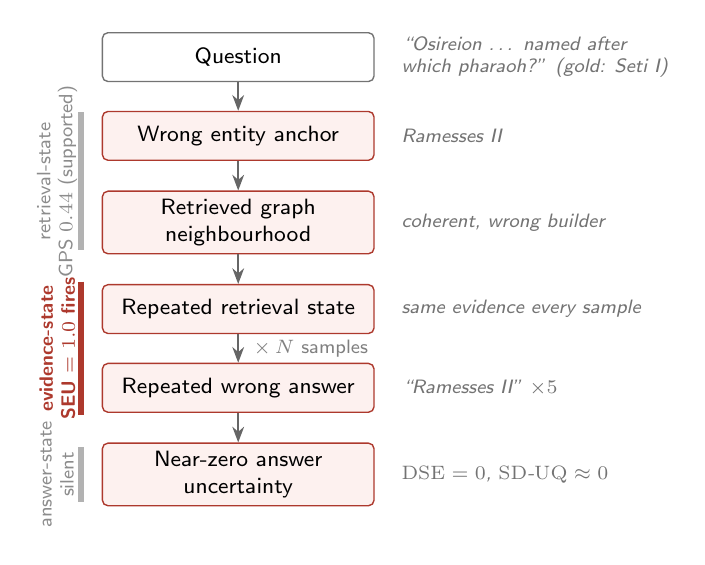
\begin{tikzpicture}[
  font=\footnotesize\sffamily,
  >={Stealth[length=2mm,width=1.5mm]},
  stage/.style={draw=black!55, line width=0.5pt, rounded corners=2pt,
                fill=white, minimum height=0.62cm, minimum width=3.45cm,
                align=center, inner xsep=5pt, inner ysep=3pt,
                font=\footnotesize\sffamily},
  bad/.style={stage, draw=badred!75!black, fill=badred!8},
  note/.style={font=\scriptsize\itshape\sffamily, text=black!55,
               align=left, anchor=west},
  raillab/.style={font=\scriptsize\sffamily, align=center, rotate=90},
  flow/.style={->, line width=0.55pt, black!60},
]
\node[stage] (q)    at (0,0)     {Question};
\node[bad]   (anc)  at (0,-1.0)  {Wrong entity anchor};
\node[bad]   (nbh)  at (0,-2.1)  {Retrieved graph\\neighbourhood};
\node[bad]   (ret)  at (0,-3.2)  {Repeated retrieval state};
\node[bad]   (ans)  at (0,-4.2)  {Repeated wrong answer};
\node[bad]   (unc)  at (0,-5.3)  {Near-zero answer\\uncertainty};

\draw[flow] (q) -- (anc);
\draw[flow] (anc) -- (nbh);
\draw[flow] (nbh) -- (ret);
\draw[flow] (ret) -- (ans)
  node[midway, right=2pt, font=\scriptsize\sffamily, text=black!50]
  {$\times\,N$ samples};
\draw[flow] (ans) -- (unc);

% ── diagnostic rail: which family observes which stage ──────────────────────
% retrieval-state family: anchor + neighbourhood
\draw[line width=2.2pt, black!30]
  (-2.00,-0.70) -- (-2.00,-2.45);
\node[raillab, text=black!45] at (-2.30,-1.58)
  {retrieval-state\\GPS $0.44$ (supported)};
% evidence-state family (the one that fires): retrieval state vs answer
\draw[line width=2.2pt, badred!75!black]
  (-2.00,-2.85) -- (-2.00,-4.55);
\node[raillab, text=badred!75!black, font=\scriptsize\bfseries\sffamily]
  at (-2.30,-3.70) {evidence-state\\SEU $=1.0$ fires};
% answer-state family (silent by construction)
\draw[line width=2.2pt, black!30]
  (-2.00,-4.95) -- (-2.00,-5.65);
\node[raillab, text=black!45] at (-2.30,-5.30)
  {answer-state\\silent};

\node[note] at (1.95,0)
  {``Osireion \ldots\ named after\\which pharaoh?'' (gold: Seti~I)};
\node[note] at (1.95,-1.0) {Ramesses~II};
\node[note] at (1.95,-2.1) {coherent, wrong builder};
\node[note] at (1.95,-3.2) {same evidence every sample};
\node[note] at (1.95,-4.2) {``Ramesses~II'' $\times 5$};
\node[note] at (1.95,-5.3)
  {$\mathrm{DSE}=0$, $\mathrm{SD\text{-}UQ}\approx 0$};
\end{tikzpicture}%
}
\caption{%
  \textbf{Worked presence-lock-in trace}, instantiated with the
  HotpotQA Osireion case also listed in
  Appendix Table~\ref{tab:lockin_gallery}.
  The retriever anchors to a strongly associated but wrong entity, the
  resulting graph neighbourhood is internally coherent, every sample receives
  the same evidence, and the repeated wrong answer presents near-zero
  answer-state uncertainty.
  The left rail shows where each diagnostic family attaches: the answer-state
  family is silent by construction, GPS remains low because the wrong answer
  is reachable in the retrieved graph, and only the evidence-state signal
  fires---the retrieved passages contradict the repeated answer.
  This traces the \emph{presence} variant; in the \emph{absence} variant
  (Section~\ref{sec:results_collapse}) the chain instead repeats an empty
  retrieval state, and the warning moves to the retrieval-state abstention
  observable.%
}
\label{fig:lockin_trace}
\end{figure}


Lock-in is easier to diagnose in knowledge-graph-augmented RAG (KG-RAG),
where a symbolic retriever can repeatedly anchor to the same entity and
traverse the same relation path.
Knowledge graphs can help on multi-hop or provenance-sensitive tasks
\citep{edge2024graphrag,gutierrez2024hipporag,hu2025grag,shen2025gear,zhu2025kg2rag,wu2025medgraphrag}.
Recent comparisons, however, find graph retrieval task-dependent and often
complementary to flat dense retrieval rather than universally superior
\citep{zhang2025ragvsgraphrag,xiang2025whengraphs,
chen2025comparingraggraphrag,peng2024graphragsurvey}.
That same symbolic structure can sharpen the failure mode, because entity-first
retrieval may keep returning the same wrong neighbourhood.

The symptom is not limited to graphs. Any system that repeatedly returns a
concentrated evidence set can produce stable wrong answers, but KG-RAG is
useful here because its retrieval state is visible: matched entities,
triples, paths, and anchors make the mechanism observable rather than merely
suspected.
The experiments use \system{},\footnote{\url{https://github.com/julka01/OntoGraphRAG}}
an ontology-guided KG-RAG framework with
entity-first routing, dense fallback, provenance-aware evidence assembly, and
graph-state logging, as the experimental setting in which to measure and
characterise lock-in.

\paragraph{Three distinct uncertainty objects.}
The central claim is that RAG confidence has three distinct objects:
\begin{enumerate}
  \item \textbf{Answer-state uncertainty} measures variation across sampled
  answers.
  \item \textbf{Evidence-state uncertainty} measures whether the retrieved
  passages locally support the generated answer.
  \item \textbf{Retrieval-state uncertainty} measures whether the retrieval
  state itself supplies graph support.
\end{enumerate}
These families are not causally independent; they are useful because each
attaches to a different object in the pipeline: the answer, the evidence, and
the retrieval state.
The triad is used throughout.\footnote{Some figures and artefact names use the
aliases \emph{output}, \emph{grounding}, and \emph{structural}.}
Each also maps to a practical trust question for deployed systems: calibrated
confidence, faithfulness to retrieved evidence, and auditable provenance.

\paragraph{Contributions.}
First, the analysis \textbf{measures the silent-error footprint compatible with
retrieval-state lock-in} under deployable policies, not only in strict stress
tests: $42\%$ of adaptive KG errors and $59\%$ of dense-retrieval errors
carry zero observed answer-state uncertainty at the operational $N{=}5$ sampling
budget, so a score using only within-question answer dispersion has no
disagreement signal to exploit: a family-level blind spot, not a stress-test
artefact.
Second, it introduces a \textbf{diagnostic decomposition} that separates
answer-state, evidence-state, and retrieval-state uncertainty.
Within the answer-state family, it also introduces SD-UQ, a low-cost
question-conditioned embedding-dispersion score that is competitive in these
low-sample RAG runs, while showing that even stronger answer-state scores cannot
diagnose lock-in alone.
The answer-state and evidence-state families are implemented directly; the
retrieval-state family is represented by a conditional graph-support
diagnostic (GPS, soft-linked and depth-matched, reported in risk orientation:
lower means stronger graph support).
Their representative scores are weakly correlated in practice (pooled Spearman
$\rho=0.03$ between answer- and evidence-state), so they carry complementary
signal rather than restating one scalar.
Third, it provides \textbf{stress-test evidence}: a strict graph-only probe
drives answer-state AUROC down to $0.233$ ($-0.52$ versus adaptive KG under
paired bootstrap), and route logs localise much of the silent error mass to
repeated empty retrieval states.
Fourth, it reports a \textbf{controlled empirical study} across five QA
families and distils the decomposition into a \textbf{conjunctive low-risk
audit rule}: treating an answer as low-risk only when all three families concur
selects a low-risk subset at $91.9\%$ pooled accuracy against a $69.7\%$ base
rate, and at $100\%$ precision under the automated judge on the clinical target
domain at $22\%$ coverage (Section~\ref{sec:results_composite}).

To separate deployment behaviour from the stress regime, the experiments compare
dense RAG, adaptive KG-RAG, and a strict graph-only KG stress test across clinical,
biomedical, and open-domain multi-hop QA snapshots.
The adaptive setting is the practical policy. The strict graph-only setting is
a mechanism probe, not a proposed retriever.
The results are mixed by design: adaptive KG retrieval is close to dense
retrieval accuracy on several snapshots (e.g., $0.946$ vs.\ $0.950$ on
RealMedQA) but does not universally improve it.
That is the condition under which the diagnostic contribution becomes precise:
when accuracy parity holds, what matters is what the retrieval layer makes
visible.

These pieces lead to the audit rule evaluated in
Section~\ref{sec:results_composite}.

\paragraph{Scope.}
Three boundaries constrain the claims below.
(1)~The absence/presence route decomposition depends on the symbolic retrieval
state that \system{} exposes; the silent-error phenomenon itself is not
graph-specific.
(2)~The strict graph-only stress test changes several pipeline components at
once, so it bounds a regime rather than isolating a single causal variable.
(3)~The fixed-subset evaluation estimates diagnostic behaviour, not lock-in
prevalence in deployed systems.

\section{Related Work}
\label{sec:related_work}

\subsection{Answer-State Uncertainty for LLMs}

A large part of LLM uncertainty estimation operates in output space.
Semantic entropy clusters sampled responses into meaning-equivalent groups and
computes entropy over the resulting distribution
\citep{kuhn2023semantic,farquhar2024detecting}.
Related methods simplify or approximate that idea:
SEP predicts semantic entropy from hidden states \citep{kossen2024sep},
SelfCheckGPT uses contradiction across samples \citep{manakul2023selfcheckgpt},
and \textsc{P(True)} asks the model to verbalise its own confidence
\citep{kadavath2022language}.
The same answer-agreement intuition underlies self-consistency decoding, where
agreement across sampled reasoning paths is read as a correctness signal
\citep{wang2023selfconsistency}.
SEP is relevant but requires white-box hidden-state access, which the present
black-box setting does not provide.
More recent white-box methods such as induction-aware entropy gating
\citep{bazarova2026intrygue}, which modulates entropy by induction-head
activity, are likewise out of scope here but orthogonal: such a mechanistic
signal could be fused with retrieval-state diagnostics rather than competing
with them.

A second line of work uses response-embedding geometry rather than hard
semantic clustering.
Kernel Language Entropy measures von~Neumann entropy on a similarity kernel
\citep{nikitin2024kernellanguageentropy}; Semantic Density and Semantic
Volume quantify concentration and dispersion in embedding space
\citep{qiu2024semanticdensity,li2025semanticvolume}; and
\citet{walha2025finegrained} decompose representation uncertainty with a
spectral formulation.
These methods are the closest answer-state baselines for the family studied
here. Their limitation for the present setting is one of scope, not quality:
they were developed for answer variation itself, not for regimes where
retrieval may stabilise around an explicit graph trace.

\subsection{Uncertainty in RAG}

RAG uses uncertainty in several ways.
Adaptive retrieval methods use confidence or entropy to decide when retrieval
should occur
\citep{jiang2023active,su2024dragin,yao2025seakr,liu2025ctrla,zubkova2025sugar},
while others import standalone LLM uncertainty estimators as retrieval triggers
or answer-confidence scores
\citep{moskvoretskii2025adaptive}.
This connects to selective prediction and abstention
\citep{geifman2017selective,tomani2024abstention}, conformal NLP
\citep{campos2024conformalnlp}, and RAG trustworthiness work that treats
reliability as a pipeline property rather than a generator property
\citep{sun2024trustllm,ni2025trustworthyrag}.
Conformal methods derive a formal coverage guarantee from a single
nonconformity score; the conjunctive audit rule introduced here instead
requires three signal families to agree and targets auditable abstention rather
than formal coverage calibration.
This literature shows that uncertainty is already operational in RAG,
but many deployment-facing designs still reduce it to one routing or
abstention scalar rather than reporting answer, evidence, and retrieval-state
behaviour separately.
These answer-side gates trigger retrieval from sampled-answer
uncertainty, the very signal that lock-in silences, so they compose with
rather than replace the evidence- and retrieval-state diagnostics studied here.
A complementary line predicts evidence quality directly:
\citet{perezbeltrachini2025passageutility} train a lightweight passage-utility
model for a target QA system, approximating sampling-based uncertainty without
sampling, a learned counterpart to the evidence-state signal whose
head-to-head against SEU is a logical next comparison.
A neighbouring self-reflective line asks the model itself to decide when to
retrieve, critique, or abstain, often through learned control tokens,
fine-tuning, or model-specific prompting policies.
Self-RAG trains reflection tokens for retrieve/generate/critique decisions;
corrective RAG evaluates retrieved document quality and triggers corrective
retrieval \citep{asai2024selfrag,yan2024crag}.
Self-RAG and corrective RAG need white-box access for fine-tuning or control
tokens; the present design instead emphasises black-box diagnostics, because
clinical and biomedical deployments often sit behind hosted models, locked
APIs, or governance constraints that rule out hidden-state probes and
task-specific fine-tuning.

Several recent papers move closer to the present perspective.
An axiomatic analysis shows that standard uncertainty estimators cannot reliably
assess correctness in RAG and proposes a calibration framework to address it
\citep{soudani2025axiomaticrag}; the present study is the empirical counterpart,
locating where answer-state agreement collapses and which retrieval- and
evidence-state signals still respond.
FRANQ separates factuality from faithfulness to retrieved context,
but it operates on flat-text RAG and does not expose three-way graph-side
decomposition \citep{fadeeva2025franq}.
SURE-RAG scores evidence-set sufficiency for selective answering
\citep{qiu2026surerag}, the evidence-state question asked well, but not
whether retrieval itself has concentrated around a wrong symbolic trace.
R2C perturbs the retrieval--reasoning loop so that dispersion under
paraphrases, rethinking, and validation reflects both retriever and generator
uncertainty \citep{soudani2025uqretrievalreasoning}.
It is complementary: R2C measures movement under perturbation, while lock-in
concerns unperturbed retrieval that barely moves at all.
This also connects to retrieval-stability and context-selection work more
broadly.
Long-context RAG and context-balancing methods ask which spans should be kept
or loaded \citep{li2024uncertaintyrag,voloshyn2026lrag}; noise-aware
calibration studies how irrelevant retrieved context affects confidence
\citep{liu2026nacc}; and retriever benchmarks study how much information the
retrieved set carries \citep{zheng2026revisitingrag}.
Those papers establish that retrieval composition matters for reliability.
The present claim is narrower: when repeated samples see the same defective
state, answer variance can collapse even if the generator is sampled.
Ca2KG studies overconfidence in KG-RAG through counterfactual prompting,
but it does not report a structured multi-family diagnostic pipeline
\citep{ren2026ca2kg}.
BRINK shows that KG-RAG systems can fall back on parametric memory when
graphs are incomplete \citep{zhou2025brink}; here the absence/presence split
is retrieval-time and is separated empirically in
Section~\ref{sec:results_collapse}.
Table~\ref{tab:positioning} summarises the positioning against these five
closest neighbours.
A direct empirical head-to-head against them is out of scope here: FRANQ,
SURE-RAG, and R2C target flat-text RAG and are reported on different corpora,
retrievers, and answer formats, so a like-for-like comparison would mean
reimplementing each inside the KG-RAG pipeline.
The contribution is the graph-side three-family decomposition and the lock-in
diagnosis, which is orthogonal to and composable with those evidence- and
perturbation-based scores; a controlled head-to-head, especially against
learned passage-utility predictors, is the natural next study.

\begin{table}[t]
\centering
\footnotesize
\setlength{\tabcolsep}{2.8pt}
\caption{%
  \textbf{Positioning against the closest related work}
  (citations in the text above).
  \checkmark{}: a direct object of study; $\sim$: partial or indirect
  (e.g., perturbation-based rather than state-inspecting); --: not
  addressed.
  \emph{Trace} denotes whether the symbolic retrieval state (anchors,
  paths, triples) is exposed for inspection; \emph{lock-in} denotes whether
  the concentrated-wrong-retrieval regime itself is studied.
  Among these five recent neighbours, the present study is the only one marked
  across all five columns.%
}
\label{tab:positioning}
\begin{tabular}{@{}lccccc@{}}
\toprule
& Answer & Evidence & Retrieval & Trace & Lock-in \\
& state & state & state & exposed & studied \\
\midrule
FRANQ & \checkmark & \checkmark & -- & -- & -- \\
SURE-RAG & -- & \checkmark & $\sim$ & -- & -- \\
R2C & \checkmark & $\sim$ & $\sim$ & -- & -- \\
Ca2KG & \checkmark & -- & $\sim$ & $\sim$ & -- \\
BRINK & -- & -- & $\sim$ & $\sim$ & -- \\
This paper & \checkmark & \checkmark & \checkmark & \checkmark & \checkmark \\
\bottomrule
\end{tabular}
\end{table}
Noise-aware calibration and long-context RAG work show that retrieval can
create uncertainty beyond decoding alone
\citep{liu2026nacc,li2024uncertaintyrag}, and evaluation frameworks such as
RAGAs and ARES foreground context relevance and faithfulness alongside answer
quality \citep{es2024ragas,saadfalcon2024ares}.
RAG evaluation has separated signals before; the narrower contribution here is
to connect that separation to explicit graph retrieval state, where answer
agreement and evidence support can decouple with measurable consequences for
uncertainty quality.
Several of these evaluator families are already represented inside the
eight-metric suite benchmarked here, semantic entropy and SelfCheckGPT
(sampling and cross-sample consistency), a perturbation-sensitivity score
(SRE-UQ), a calibration proxy (P(True)), and a RAGAs-style answer-support score
(SEU), so the comparison is in part internal rather than absent.
What remains for a dedicated head-to-head is the learned and full-pipeline
systems (passage-utility predictors, FRANQ, SURE-RAG, R2C, and ARES-style
frameworks), each of which targets flat-text RAG and would have to be
reimplemented inside the KG-RAG pipeline to compare like for like.
This also relates to internal--external conflict, where retrieved evidence
supports one answer while the model prior favours another.
ClashEval and recent conflict-aware RAG systems model that tension through
source-aware synthesis, fact-level conflict modelling, or KG-mediated
reconciliation
\citep{wu2024clasheval,wang2025astuterag,zhang2025faithfulrag,liu2025truthfulrag}.
Recent attribution work makes a related distinction between a citation that is
correctly supportive and one the model relied upon
\citep{wallat2025faithfulness}.
The present study asks which signals remain useful when retrieval is
visible and partially stabilised.

\subsection{KG-RAG and Graph-Side Uncertainty}

Graph-augmented retrieval has become a major alternative to flat-text RAG.
Systems such as RoG, Think-on-Graph, HippoRAG, SubgraphRAG, and GraphRAG use
graphs to make multi-hop reasoning more explicit, decomposable, and auditable
\citep{luo2024rog,sun2024tog,ma2025tog2,gutierrez2024hipporag,
li2025subgraphrag,edge2024graphrag}.
Their benefits tend to appear on tasks requiring multi-hop retrieval, bridge
preservation, networked evidence organisation, or stronger provenance
\citep{edge2024graphrag,gutierrez2024hipporag,shen2025gear,
hu2025grag,zhu2025kg2rag,wu2025medgraphrag}.
Topology-aware retrieval makes a related point from the retrieval side: texts
can be selected by graph proximity and structural role, not only lexical or
embedding similarity \citep{wang2024taar}.
This study treats the graph as a source-linked summary of passages: triples,
paths, and relation anchors matter because they trace back to the text that
licensed them.
Comparative work correspondingly suggests that graph and dense retrievers are
often complementary rather than globally ordered
\citep{zhang2025ragvsgraphrag,xiang2025whengraphs,peng2024graphragsurvey,
chen2025comparingraggraphrag}.

What remains comparatively underdeveloped is graph-side confidence
analysis: scoring whether the retrieved graph state itself, its matched
entities, traversal paths, and relation anchors, supports the generated answer,
rather than checking answer variation or text-evidence consistency.
Ca2KG studies overconfidence in KG-RAG through counterfactual prompting
\citep{ren2026ca2kg}, and BRINK shows that KG-RAG systems can lean on
parametric memory when retrieved graphs are incomplete \citep{zhou2025brink}.
A separate literature models uncertainty inside knowledge graphs themselves,
for example with confidence-weighted triples or distribution shift in KG
embeddings \citep{takahashi2025uncertaintyawarekg,
lee2025decomposinguncertaintykge,zhu2025certainty}.
The diagnostic question is how to score answer variation, evidence support, and
graph support once a hybrid KG-RAG system exposes all three.

\section{Background and Problem Formulation}
\label{sec:background}

\subsection{Sampling-Based Uncertainty in RAG}
\label{sec:uq_background}

Let $q$ be a question, $c$ a retrieved context, and $r$ a model response.
Sampling-based uncertainty estimators operate on repeated draws from
$p(r \mid q)$.
In RAG, however, the response distribution is mediated by retrieval:
\begin{equation}
  p(r \mid q)
  = \sum_{c \in \mathcal{C}(q)} p(r \mid q, c)\, p(c \mid q),
  \label{eq:marginal}
\end{equation}
where $\mathcal{C}(q)$ is the finite set of candidate contexts the corpus and
retrieval policy make available for question $q$.
In words, the response distribution is a mixture over the contexts the
retriever might return, weighted by their retrieval probability.
Methods such as semantic entropy therefore reflect both decoder stochasticity
and whatever variability retrieval introduces.
In vanilla RAG this can be useful: different top-$k$ chunks yield different
answers when evidence is weak or unstable.

\subsection{Why KG-RAG Changes the Interpretation}
\label{sec:determinism}

KG-RAG changes how that disagreement should be read.
Vanilla RAG returns a ranked list of passages; KG-RAG can return a structured
state whose elements have names and types, encoding claims as triples
$(\mathrm{subject}, \mathrm{relation}, \mathrm{object})$.
Anchors, relation labels, triples, paths, and the passages that license them
are checkable intermediate objects, not merely more prompt text.
In the entity-first regime studied here, retrieval is mediated by entity
matching and graph expansion over a fixed graph $\mathcal{G}$.
When that process is highly stabilised, one question-conditioned context can
dominate:
\begin{equation}
  c^\star = \arg\max_{c \in \mathcal{C}(q)} p(c \mid q).
\end{equation}
As the residual mass $1 - p(c^\star \mid q)$ shrinks, the marginal in
Equation~\eqref{eq:marginal} is dominated by a single term,
\begin{equation}
  p(r \mid q) \approx p(r \mid q, c^\star),
  \label{eq:collapsed}
\end{equation}
and repeated samples mostly expose decoder variability under fixed evidence
(Appendix~\ref{sec:appendix_residual_bound} gives the corresponding
total-variation bound for the small-residual regime).
Equation~\eqref{eq:collapsed} is a stylised limit, not a claim about KG-RAG
as a category, and the experiments do not estimate $p(c \mid q)$ directly.
It formalises the regime of interest: once retrieval stabilises, low answer
variance can mean either good evidence or the same retrieval-side mistake on
every sample.

\subsection{A Three-Family Analysis Frame for KG-RAG}
\label{sec:decomposition}

% Figure: Pipeline-aligned diagnostic objects.
% Single-column (figure). Include with: % Figure: Pipeline-aligned diagnostic objects.
% Single-column (figure). Include with: \input{figures/decomposition}

\begin{table}[t]
\centering
\small
\setlength{\tabcolsep}{5pt}
\renewcommand{\arraystretch}{1.35}
\begin{tabular}{@{}p{0.19\linewidth}p{0.27\linewidth}p{0.42\linewidth}@{}}
\toprule
\textbf{Observed object} & \textbf{Signal family} & \textbf{Diagnostic question} \\
\midrule
Answer samples
&
Answer-state uncertainty
&
Do repeated generations disagree, or has the answer surface become
artificially stable? \\
\addlinespace[0.25em]
Retrieved passages
&
Evidence-state uncertainty
&
Does the retrieved text locally entail, contradict, or fail to support the
generated answer? \\
\addlinespace[0.25em]
Graph trace
&
Retrieval-state uncertainty
&
Which anchors, typed triples, and paths made the answer reachable, and where
does the graph abstain? \\
\bottomrule
\end{tabular}

\vspace{0.45em}
\begin{minipage}{0.96\linewidth}
\footnotesize
\textit{The families are not independent causes of correctness.}
They are separately logged views of the same KG-RAG run: generated text,
retrieved evidence, and symbolic retrieval state.
\end{minipage}

\caption{%
  \textbf{Uncertainty is treated as an audit problem over pipeline objects.}
  Answer-state metrics see only sampled answers.
  Evidence-state metrics compare the answer with retrieved passages.
  Retrieval-state diagnostics inspect the graph trace itself: anchors,
  subject--relation--object triples, paths, and abstentions.
  This is why the families are reported separately.
  This table defines the objects; Table~\ref{tab:failure_modes} states how
  each family behaves across retrieval regimes, and
  Table~\ref{tab:failure_taxonomy} maps their joint outcomes into a
  $2{\times}2$ failure taxonomy.%
}
\label{tab:decomposition}
\end{table}


\begin{table}[t]
\centering
\small
\setlength{\tabcolsep}{5pt}
\renewcommand{\arraystretch}{1.35}
\begin{tabular}{@{}p{0.19\linewidth}p{0.27\linewidth}p{0.42\linewidth}@{}}
\toprule
\textbf{Observed object} & \textbf{Signal family} & \textbf{Diagnostic question} \\
\midrule
Answer samples
&
Answer-state uncertainty
&
Do repeated generations disagree, or has the answer surface become
artificially stable? \\
\addlinespace[0.25em]
Retrieved passages
&
Evidence-state uncertainty
&
Does the retrieved text locally entail, contradict, or fail to support the
generated answer? \\
\addlinespace[0.25em]
Graph trace
&
Retrieval-state uncertainty
&
Which anchors, typed triples, and paths made the answer reachable, and where
does the graph abstain? \\
\bottomrule
\end{tabular}

\vspace{0.45em}
\begin{minipage}{0.96\linewidth}
\footnotesize
\textit{The families are not independent causes of correctness.}
They are separately logged views of the same KG-RAG run: generated text,
retrieved evidence, and symbolic retrieval state.
\end{minipage}

\caption{%
  \textbf{Uncertainty is treated as an audit problem over pipeline objects.}
  Answer-state metrics see only sampled answers.
  Evidence-state metrics compare the answer with retrieved passages.
  Retrieval-state diagnostics inspect the graph trace itself: anchors,
  subject--relation--object triples, paths, and abstentions.
  This is why the families are reported separately.
  This table defines the objects; Table~\ref{tab:failure_modes} states how
  each family behaves across retrieval regimes, and
  Table~\ref{tab:failure_taxonomy} maps their joint outcomes into a
  $2{\times}2$ failure taxonomy.%
}
\label{tab:decomposition}
\end{table}


``Uncertainty in KG-RAG'' is not a single quantity: entity anchoring, graph
expansion, evidence assembly, and generation can fail for different reasons.
The analysis tracks the three families against three observable
objects: answer, evidence, and retrieval state
(Table~\ref{tab:decomposition}).
The factorisation below is a bookkeeping device for these observable stages,
not a distinction implied by probability theory alone.
Let $s$ denote the graph retrieval state (anchors, paths, and subgraph), $c$
the textual evidence assembled from it, and $r$ the answer. The pipeline is
then
\begin{equation}
  p(r, c, s \mid q) = p(s \mid q)\, p(c \mid q, s)\, p(r \mid q, c, s).
\end{equation}
Answer-state uncertainty primarily probes variability in $p(r \mid q, c, s)$;
evidence-state measures probe whether the produced evidence $c$ is locally
consistent with the answer $r$; retrieval-state measures probe whether the
retrieval state $s$ supplies coherent graph support in the first place.
These are consistency diagnostics over the retrieved state, not direct
correctness tests, and the split is not a claim of independence: evidence-state
signals depend on retrieval, retrieval-state scores depend on entity extraction
and graph coverage, and answer variation depends on retrieval stability.
It is a reporting partition, not a causal ontology; a system may produce
low-variance answers from the wrong subgraph, retrieve a plausible path whose
passages do not entail the answer, or retrieve good evidence while the answer
remains unstable.

\section{System Description}
\label{sec:system}

The experimental platform is \system{}, an open-source framework that exposes
both vanilla RAG and KG-RAG under a shared interface.
The two systems use the same corpora, embeddings, and generation model; they
differ only in retrieval and evidence organisation.

\begin{figure*}[t]
\centering
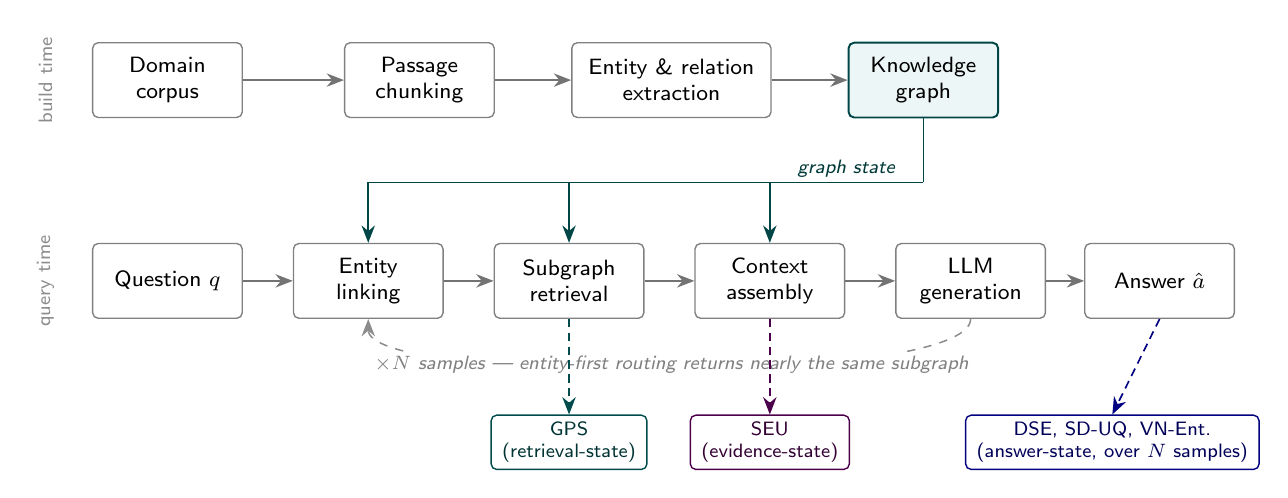
\begin{tikzpicture}[
  font=\footnotesize\sffamily,
  >={Stealth[length=2.2mm,width=1.7mm]},
  stage/.style={draw=black!50, line width=0.5pt, rounded corners=2pt,
                fill=white, minimum height=0.95cm, minimum width=1.9cm,
                align=center, inner xsep=6pt, inner ysep=4pt},
  kgstage/.style={stage, draw=teal!55!black, line width=0.7pt, fill=teal!7},
  flow/.style={->, line width=0.55pt, black!55},
  rail/.style={teal!55!black, line width=0.55pt},
  rowlab/.style={font=\scriptsize\sffamily, text=black!45},
]

%% ── Build row ────────────────────────────────────────────────────────────────
\node[stage]   (corpus)  at (0,2.55)   {Domain\\corpus};
\node[stage]   (chunk)   at (3.2,2.55) {Passage\\chunking};
\node[stage]   (extract) at (6.4,2.55) {Entity \& relation\\extraction};
\node[kgstage] (kg)      at (9.6,2.55) {Knowledge\\graph};

%% ── Query row ────────────────────────────────────────────────────────────────
\node[stage] (q)    at (0,0)     {Question $q$};
\node[stage] (link) at (2.55,0)  {Entity\\linking};
\node[stage] (sub)  at (5.1,0)   {Subgraph\\retrieval};
\node[stage] (ctx)  at (7.65,0)  {Context\\assembly};
\node[stage] (llm)  at (10.2,0)  {LLM\\generation};
\node[stage] (ans)  at (12.6,0)  {Answer $\hat{a}$};

%% ── Row labels ───────────────────────────────────────────────────────────────
\node[rowlab, rotate=90, anchor=center] at (-1.55,2.55) {build time};
\node[rowlab, rotate=90, anchor=center] at (-1.55,0)    {query time};

%% ── Flow arrows ──────────────────────────────────────────────────────────────
\draw[flow] (corpus) -- (chunk);
\draw[flow] (chunk)  -- (extract);
\draw[flow] (extract) -- (kg);
\draw[flow] (q)    -- (link);
\draw[flow] (link) -- (sub);
\draw[flow] (sub)  -- (ctx);
\draw[flow] (ctx)  -- (llm);
\draw[flow] (llm)  -- (ans);

%% ── Graph-state rail: the KG conditions three query-time stages ──────────────
\coordinate (raily) at (0,1.25);
\draw[rail] (kg.south) -- (kg.south |- raily);
\draw[rail] (link.north |- raily) -- (kg.south |- raily);
\draw[->, rail] (link.north |- raily) -- (link.north);
\draw[->, rail] (sub.north  |- raily) -- (sub.north);
\draw[->, rail] (ctx.north  |- raily) -- (ctx.north);
\node[font=\scriptsize\itshape\sffamily, text=teal!45!black,
      above, inner sep=1.5pt] at (8.62,1.25) {graph state};

%% ── Sampling loop: N samples re-enter retrieval, returning ~the same state ──
\draw[dashed, line width=0.55pt, black!45, ->]
  (llm.south) .. controls +(0,-0.85) and +(0,-0.85) .. (link.south);
\node[font=\scriptsize\itshape\sffamily, text=black!50, fill=white,
      inner sep=1.5pt] at (6.4,-1.07)
  {$\times N$ samples --- entity-first routing returns nearly the same subgraph};

%% ── Measurement taps: where each diagnostic family attaches ─────────────────
\tikzset{tap/.style={draw, line width=0.5pt, rounded corners=2pt,
                     align=center, font=\scriptsize\sffamily,
                     inner xsep=4pt, inner ysep=2.5pt, fill=white},
         probe/.style={densely dashed, line width=0.6pt, ->}}
\node[tap, draw=teal!60!black, text=teal!40!black] (tgps) at (5.1,-2.05)
  {GPS\\(retrieval-state)};
\node[tap, draw=violet!60!black, text=violet!40!black] (tseu) at (7.65,-2.05)
  {SEU\\(evidence-state)};
\node[tap, draw=blue!50!black, text=blue!35!black] (tans) at (12.0,-2.05)
  {DSE, SD-UQ, VN-Ent.\\(answer-state, over $N$ samples)};
\draw[probe, teal!60!black]   (sub.south) -- (tgps.north);
\draw[probe, violet!60!black] (ctx.south) -- (tseu.north);
\draw[probe, blue!50!black]   (ans.south) -- (tans.north);

\end{tikzpicture}
\caption{%
  \textbf{\system{} pipeline with the three measurement taps.}
  \emph{Build time} (top): a domain corpus is chunked and converted via
  ontology-guided extraction into a typed knowledge graph with passage-level
  provenance.
  \emph{Query time} (bottom): the question is linked to seed entities, and the
  graph state conditions retrieval at three points---entity linking, subgraph
  traversal, and context assembly---before the LLM produces the final answer.
  The dashed probes mark where each diagnostic family attaches: GPS scores
  graph support in risk orientation, SEU scores the assembled evidence against
  the answer, and the answer-state estimators see only the $N$ sampled answers.
  The sampling loop is the lock-in mechanism: each of the $N$ samples re-enters
  retrieval, and entity-first routing returns nearly the same subgraph, so
  answer-state uncertainty mostly reflects decoder noise under almost-fixed
  evidence (Section~\ref{sec:metrics}).%
}
\label{fig:pipeline}
\end{figure*}


\subsection{\system{} Overview}
\label{sec:ontographrag_overview}

\system{} is designed around a simple principle: graph retrieval should add
structure without discarding dense evidence (Figure~\ref{fig:pipeline}).
The graph makes retrieval commitments explicit: recognised entities, accepted
relations, triples, paths, and licensing passages.
During KG construction, passages are converted into entity and relation nodes
with ontology-guided typing, anchor grounding, confidence scores, provenance
links, and contradiction flags when a schema is available.
During retrieval, the system first tries to route the question through matched
entities and local graph neighbourhoods.
When the anchor is weak, it uses dense retrieval and retriever-first graph
expansion as fallback.
The resulting context contains both textual passages and explicit graph paths,
so the answer can be evaluated at three levels: the answer state, the
evidence state, and the retrieval state.
\system{} logs anchors, paths, and supporting passages with the final answer,
so the provenance trace is part of the retrieval output, not a private prompt
construction detail.

\subsection{Vanilla RAG}
\label{sec:vanilla_rag}

Vanilla RAG performs direct vector retrieval over chunk embeddings.
For each question, it retrieves the top-$k$ chunks above a similarity
threshold and optionally appends adjacent chunks to capture answers split
across chunk boundaries.
The LLM therefore receives flat text only.
It has no explicit entities, relations, or multi-hop paths, and thus no
graph-side object on which to define retrieval-state diagnostics.

\subsection{KG-RAG}
\label{sec:kg_rag}

KG-RAG replaces flat retrieval with a routed hybrid pipeline rather than a
single graph walk.

\paragraph{Stage 1: seed selection.}
The preferred path is entity-first anchoring: the system identifies seed
entities with symbolic matching and embedding lookup over short mentions.
If no reliable anchor is found, the system does not immediately reduce to
vector-only retrieval; instead it can route to a retriever-first graph pass.

\paragraph{Stage 2: local graph expansion and scoring.}
Starting from the seed entities, the system traverses the graph up to a
dataset-specific hop limit, producing an explicit retrieval state of linked
chunks, entities, relations, and readable traversal paths.
Traversal is provenance-aware: on question-bundle datasets, paths and edges are
restricted to the current question's local evidence rather than allowed to
borrow support from other questions in the same dataset graph.
Chunks are scored by hop distance and local diffusion over the retrieved
entity subgraph.

\paragraph{Stage 3: retriever-first graph expansion when anchoring is weak.}
When entity-first retrieval is weak or empty, the system first retrieves dense
text chunks, extracts their linked entities, expands the graph from those
passage-derived seeds, and re-scores the resulting context with a combined
vector-plus-graph signal.

\paragraph{Stage 4: evidence organisation.}
The final prompt is not a flat mixture of chunks and graph paths.
Instead, retrieved graph paths are grouped with overlapping supporting passages
into explicit reasoning chains, with remaining passages listed separately as
additional evidence.
The generator sees both structured multi-hop support and the local text that
grounds each chain.

\paragraph{Diagnostic role.}
\system{} is useful here because it makes the retrieval state explicit rather
than tacit.
The graph is not treated as an oracle; it is an auditable substrate whose
triples and paths may be helpful or wrong, but are diagnostically richer than
an unstructured list of nearest-neighbour chunks.
Because the system logs which entities were matched, which paths were
traversed, and which route was taken, the retrieval state is an explicit,
queryable object rather than an internal variable.

\paragraph{Retrieval stabilisation.}
The diagnostic question arises when the retrieval state is stable across
repeated calls; retriever-first expansion, vector fallback, and iterative
decomposition can weaken that stabilisation when the graph anchor is brittle,
so the experiments compare diagnostics across retrieval regimes.
Entity-first retrieval can be especially prone to stabilising: once the system
commits to an anchor entity, the subsequent graph expansion is largely
determined, so the same neighbourhood, right or wrong, tends to recur across
samples.

\section{Uncertainty Measures}
\label{sec:metrics}

Eight diagnostic measures are evaluated across three observable objects in a
QA episode: sampled answers, retrieved graph state, and retrieved evidence
(Table~\ref{tab:metric_taxonomy}).
They are not eight independent estimates of one hidden confidence variable.
Within-family dependencies are explicit: the P(True)-style proxy is monotone
in DSE under black-box sampling, and VN-Entropy and SD-UQ are both geometric
statistics of the same response matrix.
The headline tables report family representatives rather than treating all
eight rows as separate evidence.
The answer-state scores mostly come from standalone LLM uncertainty
\citep{kuhn2023semantic,manakul2023selfcheckgpt,kadavath2022language,moskvoretskii2025adaptive};
the retrieval- and evidence-state scores ask whether the generated answer is
reachable in the graph and supported by the retrieved text.
Let $\bm{r} = \{r_1,\ldots,r_N\}$ denote $N$ responses sampled from the
LLM for a question $q$ with retrieved context $c$.
Let $\bm{v}_i \in \mathbb{R}^d$ denote the $\ell_2$-normalised embedding of
$r_i$, and $\bm{V} = [\bm{v}_1\mid\cdots\mid\bm{v}_N]^\top \in \mathbb{R}^{N\times d}$
the stacked response embedding matrix.
All estimators return a non-negative scalar with higher values indicating
greater uncertainty.
The retrieval-state diagnostic GPS and the evidence-state estimator SEU are
bounded in $[0,1]$; DSE and VN-Entropy have maximum $\log N$; SRE-UQ and
SD-UQ are non-negative and unbounded.
Because the experiments use only $N=5$ samples, the answer-state estimators are
low-sample operational diagnostics, not high-precision distribution estimates.

\begin{table*}[t]
\centering
\small
\caption{%
  \textbf{Taxonomy of the eight uncertainty measures.}
  The first six rows are answer-state estimators; the last two instantiate
  retrieval-state and evidence-state diagnostics.
  Measured per-question costs are reported in Appendix
  Table~\ref{tab:compute_cost}.
  $\dagger$: metric or KG-RAG operationalisation defined here.
  $\ddagger$: prior estimator first benchmarked here for KG-RAG.%
}
\label{tab:metric_taxonomy}
\begin{tabular}{@{}llp{5.2cm}p{2.9cm}p{2.7cm}@{}}
\toprule
\textbf{Family} & \textbf{Measure} & \textbf{Formal sketch} & \textbf{Required inputs} & \textbf{Cost at inference} \\
\midrule
Entropy
  & DSE
  & $-\sum_k \hat{p}_k \log \hat{p}_k$, with $\hat{p}_k = |C_k|/N$
  & sampled answers, NLI
  & $N$ samples; $O(N^2)$ NLI calls \\
\midrule
Calibration
  & $\mathrm{P(True)}$
  & $1 - |\{i:\mathrm{cl}(r_i)=\mathrm{cl}(r_1)\}|/N$; black-box P(True)-style proxy
  & sampled answers, NLI
  & $N$ samples; shares DSE clustering \\
\midrule
Similarity
  & SelfCheckGPT
  & $\frac{1}{|\mathcal{P}|}\sum_{(i,j)\in\mathcal{P}}
      [\mathrm{NLI}(r_i,r_j)=\textsc{contradiction}]$
  & sampled answers, NLI
  & $N$ samples; $O(N^2)$ NLI calls \\
\midrule
Perturbation
  & SRE-UQ
  & $\frac{1}{M}\sum_{i\in\mathcal{T}}|\Delta_i|$; perturbation sensitivity of the kernel mean embedding
  & sampled answer embeddings
  & $N$ samples; embeddings only \\
\midrule
\multirow{2}{*}{Geometric}
  & VN-Entropy$^{\ddagger}$
  & $-\operatorname{tr}(\bm{\rho}\log\bm{\rho})$, with $\bm{\rho}=\bm{V}\bm{V}^\top/N$
  & sampled answer embeddings
  & $N$ samples; embeddings only \\
  & SD-UQ$^\dagger$
  & $\exp\!\bigl(\frac{1}{k}\sum_{i=1}^k \log(\eta_i+\varepsilon)\bigr)$ on question-orthogonal residuals
  & question embedding, sampled answer embeddings
  & $N$ samples; embeddings only \\
\midrule
Retrieval-state
  & GPS$^\dagger$
  & $\displaystyle 1 -
     \frac{\sum_{e:\mathrm{reach}_e} w_e \gamma^{|L_e-\hat L(q)|}}
          {\sum_e w_e}$; soft-linked, depth-matched answer-entity support
  & retrieved KG, entity embeddings, linked question/answer entities
  & 1 sample; per-entity graph queries, no LLM calls \\
\midrule
Evidence-state
  & SEU$^\dagger$
  & $\frac{1 - (n_E-n_C)/K}{2}$; entailment--contradiction deficit over retrieved chunks
  & retrieved chunks, answer, NLI
  & 1 sample; $K$ NLI calls \\
\bottomrule
\end{tabular}
\end{table*}

% =============================================================================
\subsection{Answer-State Uncertainty Estimators}
\label{sec:gen_metrics}

\paragraph{Semantic entropy and DSE.}
\citet{kuhn2023semantic} cluster sampled responses into meaning-equivalent
sets $\mathcal{C}=\{C_1,\ldots,C_K\}$ using bidirectional NLI entailment.
The API setting exposes no reliable per-sample likelihoods, so the reported
score is the count-weighted black-box variant,
\begin{equation}
  \mathrm{DSE}(\bm{r})
  = -\sum_{k=1}^{K} \frac{|C_k|}{N}\log\frac{|C_k|}{N}.
\end{equation}
DSE is semantic entropy with uniform sample weights; likelihood-weighted SE is
therefore not reported separately.

\paragraph{P(True).}
\textbf{P(True)}~\citep{kadavath2022language} is implemented as a black-box
cluster-agreement proxy: the fraction of samples in the same semantic cluster
as the first response
($\mathrm{P(True)}_{\mathrm{proxy}} =
|\{i: \mathrm{cl}(r_i)=\mathrm{cl}(r_1)\}|/N$);
uncertainty is $1 - \mathrm{P(True)}_{\mathrm{proxy}}$.
It is monotone in DSE here and is not treated as independent evidence.

\paragraph{SelfCheckGPT.}
\citet{manakul2023selfcheckgpt} measure the fraction of response pairs flagged
as contradictions by NLI:
\begin{equation}
  \mathrm{SCG}
  = \frac{1}{|\mathcal{P}|}
    \sum_{(i,j)\in\mathcal{P}}
    \bigl[\mathrm{NLI}(r_i,r_j)=\text{contradiction}\bigr],
\end{equation}
where $\mathcal{P}$ is the set of ordered response pairs.
For these short-answer tasks, the implementation uses whole-response NLI.

\paragraph{SRE-UQ.}
\citet{vipulanandan2026sreuq} measure perturbation sensitivity of the response
embedding distribution.
Let $\Delta_i$ denote the first-order perturbation score of response embedding
$\bm{\phi}_i$ around the weighted kernel mean embedding, using the published
bandwidth rule.
This analysis uses
$\displaystyle\mathrm{SRE\text{-}UQ}(\bm{r})
  = \frac{1}{M}\sum_{i \in \mathcal{T}} |\Delta_i|$,
where $\mathcal{T}$ indexes the $M$ highest-amplitude modes.
The estimator is imported as written; the contribution is its KG-RAG
benchmark, not a new perturbation objective.

\paragraph{VN-Entropy (KG-RAG instantiation).}
VN-Entropy measures spectral diversity of the normalised response-embedding
Gram matrix.
With $\bm{G}=\bm{V}\bm{V}^\top$ and $\bm{\rho}=\bm{G}/N$,
\begin{equation}
  \mathrm{VN\text{-}Entropy}(\bm{r}) = S(\bm{\rho})
  = -\operatorname{tr}(\bm{\rho}\log\bm{\rho})
  = -\textstyle\sum_{i=1}^{N} \lambda_i \log \lambda_i,
  \label{eq:vn_entropy}
\end{equation}
where $\{\lambda_i\}_{i=1}^N$ are the eigenvalues of $\bm{\rho}$.
$S(\bm{\rho}) = 0$ when all responses are identical and approaches $\log N$
when responses are mutually orthogonal.
This is a cosine-Gram instantiation of the VNE family introduced by Kernel
Language Entropy \citep{nikitin2024kernellanguageentropy}; the novelty lies in
the KG-RAG benchmark.


\paragraph{SD-UQ (introduced here).}
SD-UQ is a question-conditioned embedding-dispersion statistic, distinct from
\citet{qiu2024semanticdensity}'s Semantic Density.
It removes the question direction before measuring residual answer spread: if
the sampled answers point in nearly the same residual direction, dispersion is
low, the signature of a stabilised (and possibly locked-in) answer surface.
Given the unit-norm question embedding $\hat{\bm{q}}\in\mathbb{R}^d$, define
the orthogonal projector
\begin{equation}
  \bm{P}_{q}^{\perp}
  = \bm{I} - \hat{\bm{q}}\hat{\bm{q}}^\top.
\end{equation}
The projected response matrix is
\begin{equation}
  \bm{V}_{\perp} = \bm{V}\bm{P}_{q}^{\perp},
\end{equation}
where
$\bm{H} = \bm{I} - \frac{1}{N}\mathbf{1}\mathbf{1}^\top$
is the row-centering matrix.
The thin SVD of the centred projected matrix is
\begin{equation}
  \frac{\bm{H}\bm{V}_{\perp}}{\sqrt{N}}
  = \bm{U}\bm{\Sigma}\bm{W}^\top.
\end{equation}
Let $\eta_1 \geq \cdots \geq \eta_k$ be the top-$k$ singular values on
the diagonal of $\bm{\Sigma}$.
\begin{equation}
  \mathrm{SD\text{-}UQ}(\bm{r})
  \;=\;
  \exp\!\left(\frac{1}{k}\sum_{i=1}^{k} \log(\eta_i + \varepsilon)\right),
  \label{eq:sd_uq}
\end{equation}
where $k = \min(N{-}1,\, k_{\max})$ and $\varepsilon = 10^{-12}$ for
numerical stability.
At $N=5$, this is a low-sample projected-dispersion statistic, not a full
covariance estimate.
The geometric mean penalises collapse onto a single residual direction, so a
large score requires spread across several retained singular modes.
SD-UQ needs only question and answer embeddings; its attraction is operational
low cost, not mathematical ornament.

% =============================================================================
\subsection{Retrieval-State Support Diagnostics}
\label{sec:struct_metrics}

Retrieval-state diagnostics ask whether the retrieved graph contains a usable
path from the question entities to the asserted answer entity.
They matter when $p(c \mid q) \approx \delta_{c^*}$
(Section~\ref{sec:determinism}): repeated samples then see the same context,
so answer-state agreement can be high for both correct and wrong answers.
GPS is therefore a graph-support diagnostic reported in risk orientation:
lower values mean stronger graph support for the generated answer, while
higher values mean weak or absent graph support. It is not a truth label or a
logical entailment test.

Let $\mathcal{E}_q$ and $\mathcal{E}_a$ denote the sets of KG entities linked
to the question $q$ and answer $a$, respectively, filtered to
$\mathcal{E}_a \setminus \mathcal{E}_q$ to exclude trivial self-loops.
Question entities are linked by surface and fuzzy name matching.
Answer entities are linked by the same surface matcher \emph{plus} an
embedding-based soft matcher: candidate answer spans are embedded with the
retrieval encoder and linked to any entity whose name embedding has cosine
similarity at least $\tau$ to some span.
Each linked answer entity carries a link weight $w_e$: the matched cosine for
soft links and $w_e = 1$ for surface matches.

For GPS, answer entity extraction is restricted to the \emph{primary answer span}:
the first sentence of the response, truncated to 150 characters, which
prevents later explanatory text from inflating the reachable entity count.
If no usable answer entity remains after filtering and soft linking, GPS
abstains rather than returning a spurious support score.

\paragraph{Graph Path Support (GPS; retrieval-state diagnostic).}
GPS asks how strongly the answer is reachable from the question entities
within the retrieved KG, and reports the result in risk orientation as one
minus that support.
Each linked answer entity contributes distance-weighted support
$\gamma^{|L_e-\hat L(q)|}$, where $L_e$ is the shortest qualifying path
length (under the same edge-confidence and provenance filters used at
retrieval time), $\hat L(q)$ is the expected reasoning depth for the question,
and unreachable entities contribute zero:
\begin{equation}
  \mathrm{GPS}(q, a) \;=\;
  1 -
  \frac{\sum_{e \in \mathcal{E}_a} w_e\, \gamma^{|L_e-\hat L(q)|}\,
        \mathbb{1}[e\ \mathrm{reachable}]}
       {\sum_{e \in \mathcal{E}_a} w_e}.
\end{equation}
$\mathrm{GPS} = 0$ when every linked answer entity is reachable at the
expected reasoning depth (full structural support, low uncertainty);
$\mathrm{GPS} = 1$ when none are reachable within $h$ hops (no structural
support, high uncertainty); with $\gamma = 1$ the score reduces to the
unweighted unreachable-entity fraction.
The linking threshold and decay were calibrated on the RealMedQA development
run ($\tau = 0.60$, $\gamma = 0.4$) and applied frozen elsewhere; a
$5\times5$ sweep over $\tau$ and $\gamma$
(Appendix~\ref{sec:appendix_gps_sensitivity}) shows the held-out AUROCs are
stable across the grid, so the reported numbers are not an artefact of the
calibrated cell.
For 2WikiMultiHopQA and MuSiQue, $\hat L(q)$ is the logged per-question hop
count; for HotpotQA variants it is the nominal two-hop depth; for RealMedQA it
is $1$, which makes GPS identical to the calibrated one-hop-decay score on
the clinical domain.
If the system anchors to the wrong entity but traverses a locally coherent
neighbourhood, GPS can still be $0$: it scores graph support for the generated
answer, not correctness.
When no answer entities are found in the primary span (or when the
question is a direct-choice comparison), the estimator abstains and the row is
excluded from retrieval-state AUROC while being counted in the
linking-failure rate (Section~\ref{sec:grounding}).

% =============================================================================
\subsection{Evidence-State Uncertainty Measures}
\label{sec:grounding_metrics}

Evidence-state measures ask whether the retrieved passages support the answer,
so they can remain informative when sampled answers agree.
They are local answer--evidence consistency scores, not truth labels.

\paragraph{Support Entailment Uncertainty (SEU; evidence-support score).}
SEU is the normalised entailment--contradiction deficit over retrieved chunks,
close to answer-support scoring in RAGAs~\citep{es2024ragas}.

Let $c_1,\ldots,c_K$ denote the $K$ retrieved chunks and $a$ the generated answer.
Each chunk is classified by an NLI model
(\texttt{microsoft/deberta-large-mnli}; all model versions are listed in
Appendix~\ref{sec:appendix_reproducibility}):
$\ell_k \in \{E, N, C\}$ (entailment, neutral, contradiction) where
$E = \mathrm{NLI}(c_k \Rightarrow a)$.
Define the support score $s = (n_E - n_C)/K \in [-1, 1]$,
where $n_E = |\{k: \ell_k=E\}|$ and $n_C = |\{k: \ell_k=C\}|$.
\begin{equation}
  \mathrm{SEU}(q, a, \mathbf{c}) = \frac{1 - s}{2} \in [0, 1].
\end{equation}
$\mathrm{SEU} = 0.0$ when all chunks entail the answer (maximum support),
$\mathrm{SEU} = 0.5$ when chunks are all neutral (undefined support),
$\mathrm{SEU} = 1.0$ when all chunks contradict the answer (maximum conflict).
Neutral chunks therefore create a plateau at $0.5$, especially when a
general-domain NLI model declines to commit on specialist biomedical passages
(Section~\ref{sec:results_grounding}). Unlike answer-state scores, SEU needs
only one generation.

\paragraph{Faithfulness to structured provenance.}
SEU does not prove that the decoder followed the retrieved graph path.
A stricter path-faithfulness diagnostic would align answer claims to entities,
relation labels, and relation-anchor text on the retrieved paths.
The runs log those ingredients, but not sentence-level claim-to-path alignment
for every answer; path faithfulness is therefore left as a future
evidence-state diagnostic.

% =============================================================================
\subsection{Entity-Linking Quality}
\label{sec:grounding}

GPS requires matched question entities and at least one linkable answer entity.
Soft answer linking reduces abstention relative to surface matching
(Section~\ref{sec:results_structural}); yes/no answers remain a predictable
failure case.
For backward compatibility the scalar API emits a $0.5$ sentinel, but AUROC,
ECE, and precision-at-$k$ drop sentinel rows using the recorded null reason.

Entity-linking success rate $g \in [0, 1]$ measures
the fraction of content-bearing query tokens covered by matched entity names:
\begin{equation}
  g(q) = \min\!\left(1,\; \frac{|\hat{\mathcal{T}}_q^{\mathrm{cov}}|}{|\hat{\mathcal{T}}_q|}\right),
\end{equation}
where $\hat{\mathcal{T}}_q$ is the set of distinct alphanumeric content tokens
of length $\geq 4$ in $q$ (excluding stopwords), and
$\hat{\mathcal{T}}_q^{\mathrm{cov}} \subseteq \hat{\mathcal{T}}_q$ is the
subset covered by at least one matched entity name (a token $t$ is covered
when it appears as a sub-token of an entity name, or the entity name contains
$t$ as a substring).
This token-coverage score is a lightweight routing and stratification
heuristic, not an uncertainty estimator.
Appendix Table~\ref{tab:failure_modes} summarises the failure regimes of the
three families.

\section{Experimental Setup}
\label{sec:experimental_setup}

\subsection{Datasets}

The suite contains six fixed evaluation snapshots over five QA families:
biomedical control, clinical QA, and open-domain multi-hop QA
(Table~\ref{tab:datasets}).
It deliberately mixes corpus contracts: per-question bundles, per-question
source documents, and shared corpora.
The primary graph object is a passage-provenance KG built from the retrieval
corpus itself, since the question is whether \system{} preserves dense-RAG
answer quality while exposing facts, passages, relations, and retrieval state.
PubMedQA and MuSiQue use $n=100$; RealMedQA uses its full $n=230$ evaluable
set; HotpotQA, HotpotQA FullWiki, and 2WikiMultiHopQA use fixed $n=250$
subsets.

\begin{table*}[t]
\centering
\small
\caption{Evaluation datasets, corpus contracts, KG scale, and primary roles.
$h$ is the KG traversal depth; \emph{corpus} denotes the retrieval contract;
$n$ is the evaluated subset size.
$|E|$ and $|R|$ count entity nodes and typed entity--entity relations in the
dataset-scoped KG, queried from the persistent Neo4j stores used in the
reported runs.
\label{tab:datasets}}
\setlength{\tabcolsep}{3pt}
\begin{tabular}{@{}lllclrrrp{2.7cm}@{}}
\toprule
Dataset & Domain & Answer type & $h$ & Corpus & $n$ & $|E|$ & $|R|$ & Primary role \\
\midrule
PubMedQA
  & Biomedical & Yes/No/Maybe & 2 & abstract & 100 & 2{,}354 & 3{,}023 & Binary control; strong dense baseline \\
RealMedQA
  & Clinical & Free-text & 2 & shared (143) & 230 & 537 & 359 & Clinical shared-corpus grounding \\
HotpotQA \citep{yang2018hotpotqa}
  & Wikipedia & Free-text & 2 & bundle & 250 & 13{,}546 & 12{,}355 & Open-domain bridge diagnostic \\
HotpotQA FullWiki \citep{yang2018hotpotqa}
  & Wikipedia & Free-text & 2 & shared subset & 250 & 13{,}498 & 12{,}012 & Shared-corpus bridge stress test \\
2WikiMultiHopQA \citep{ho2020wikimultihopqa}
  & Wikipedia & Free-text & 2 & bundle & 250 & 8{,}328 & 7{,}187 & Bridge and comparison analysis \\
MuSiQue \citep{trivedi2022musique}
  & Wikipedia & Free-text & 4 & bundle & 100 & 15{,}440 & 24{,}858 & Hard multi-hop stress test \\
\bottomrule
\end{tabular}
\end{table*}

\textsc{RealMedQA} is the main shared-corpus clinical setting and
\textsc{HotpotQA FullWiki} a controlled Wikipedia shared-corpus stress
snapshot; the rest are closed source-document or bundle settings.
This is a conservative testbed for KG-RAG: dense retrieval sees small,
benchmark-filtered candidate sets and provides a demanding accuracy baseline.
\textsc{PubMedQA} is retained as a control; the open-domain datasets
stress bridge preservation, shared-corpus evidence selection, comparison
questions, and deeper compositional chains.

Throughout, hop count refers to the reasoning chain implied by the
question, not the number of passages supplied by the benchmark.
Explicit decomposition metadata are used where available, otherwise
dataset-specific conventions.
Hop-stratified analyses are reported as diagnostics rather than the main
table.

\paragraph{Scope.}
The experiments are fixed-subset diagnostic runs, not leaderboard submissions
or web-scale throughput benchmarks.
They support the paper's coarse family-level claims; fine-grained ranking of
neighbouring AUROC or AUREC values would require larger multi-seed sweeps.

\subsection{Model and Sampling}

All answer-generation experiments use GPT-4o-mini
\citep{openai2024gpt4omini}.
For answer-state uncertainty, $N=5$ responses are sampled at temperature
$T=1.0$.
These are low-budget black-box diagnostics: the API provides no reliable token
likelihoods, so entropy-style scores use sampled responses rather than decoder
probabilities.

KG construction is largely deterministic: entity and relation extraction use
temperature $0.0$, and benchmark passages are ingested one at a time with
chunk-level provenance.
The studied regime is stabilised entity-first retrieval with explicit fallback.

\paragraph{What is and is not isolated.}
The comparison holds the corpus, embeddings, and generation model fixed, but
does not fully isolate graph structure from retrieval stabilisation, fallback
routing, prompt organisation, or provenance grouping
(Section~\ref{sec:limitations}).
The runs report mean pairwise chunk overlap across the $N=5$ calls
(Appendix Table~\ref{tab:retrieval_overlap}); an archived 2WikiMultiHopQA
trace also supports the stability split in
Table~\ref{tab:within_adaptive_stability}.
The headline runs do not retain per-question entity- or path-overlap statistics
for every dataset, but a dedicated graph-state diversity run on HotpotQA-FullWiki
logs the full per-sample seed-entity, path, subgraph, and chunk overlap and is
analysed in Appendix~\ref{sec:appendix_diversity}.

\subsection{Correctness Labels}
\label{sec:correctness}

Correctness labels are binary.
Label-space tasks are normalised to their answer contract
(\texttt{yes}/\texttt{no}/\texttt{maybe}).
Free-text and factoid tasks use a reference-based semantic judge given the
question, gold answer, aliases where available, and model response; by default
the judge is GPT-4o-mini
(Appendix~\ref{sec:appendix_reproducibility}).
This is a benchmark answer-normalisation task rather than open-ended clinical
diagnosis: the judge decides reference-grounded semantic equivalence, for which
exact match would undercount aliases, paraphrases, and short explanatory
answers.
Same-model judging is a known limitation
\citep{zheng2023judging,panickssery2024llm}, so the labels are practical
reference-grounded judgements rather than an oracle.
An independent re-judge with a different model family (Llama-3.3-70B) on the
saved answers of every free-text run, including both headline RealMedQA runs,
HotpotQA, HotpotQA FullWiki, MuSiQue, and both 2WikiMultiHopQA runs, agrees
with the original labels on $92$--$99\%$ of answers
($\kappa = 0.52$--$0.97$, the low end being the near-ceiling-accuracy
RealMedQA adaptive run where few wrong answers make $\kappa$ unstable) and
leaves every central contrast unchanged (Section~\ref{sec:limitations}).

Two conventions matter.
Provider-side failures are recorded explicitly, so results report both
\textbf{raw accuracy} and \textbf{clean accuracy}, the latter excluding
generation failures (Appendix Table~\ref{tab:generation_failures}).
For free-text datasets, prompts elicit short explanatory answers rather than
extractive spans; semantic correctness is therefore the headline answer metric,
with EM/F1 retained only in the artefacts.

\subsection{Evaluation Metrics}

The main uncertainty metric is \textbf{AUROC}, the ranking quality for
separating correct from incorrect answers.
\textbf{AUREC} is logged as a secondary selective-prediction audit metric
\citep{geifman2017selective}, but not expanded into a parallel results table.
Raw accuracy, clean accuracy, retrieval overlap, and per-metric compute time
are also logged; the marginal cost of each diagnostic, including SEU's
per-chunk NLI calls and GPS, is reported in
Appendix Table~\ref{tab:compute_cost}.
All main figures report point estimates from one fixed subset per dataset.
With mixed sample sizes ($n=100$, $n=230$, $n=250$), small AUROC gaps are
descriptive unless they recur across signal families or match the qualitative
traces.
No multiple-comparison correction is applied because the heatmap is not used
for family-wise significance testing.
The two primary headline contrasts instead carry paired-bootstrap intervals;
the largest, the adaptive-versus-strict SD-UQ collapse of $+0.52$ AUROC at
$n=196$, is far from zero, whereas gaps near $0.05$ are not interpreted.
Appendix Tables~\ref{tab:run_artifacts}, \ref{tab:effective_denominators},
\ref{tab:hotpot_fullwiki_stress}, and \ref{tab:headline_ci_output} document
run configurations, answered counts, GPS usable counts, the HotpotQA FullWiki
snapshot, and bootstrap intervals.
Retrieval-state AUROC with fewer than roughly fifty usable rows is treated as
trace-level evidence.
GPS AUROC is always conditional on rows for which GPS is defined; linking
failures and other abstentions are reported through usable/answered
denominators and audit-rule coverage, not hidden inside the AUROC.

The headline tables report family representatives: DSE, SRE-UQ, VN-Entropy,
and SD-UQ for answer state; SEU for evidence state; GPS for retrieval state.
The P(True)-style proxy is omitted because it is monotone in DSE here, and
SelfCheckGPT is retained in the artefacts.
GPS uses surface plus embedding-based soft answer-entity linking; its two
hyperparameters were calibrated on the RealMedQA development run and frozen
elsewhere.
All GPS values were recomputed by post-hoc replay on saved answer logs without
rerunning generation, retrieval, or entity linking
(Appendix~\ref{sec:appendix_reproducibility}).
PubMedQA-style yes/no answers remain outside GPS's intended scope because they
expose no linkable answer entities.

\subsection{Retrieval and KG Configuration}

Both systems use \texttt{all-MiniLM-L6-v2}.
Vanilla RAG performs direct vector retrieval over chunks.
KG-RAG performs entity-first retrieval, graph expansion, and context assembly
from graph-linked chunks, paths, and entities, with dense retrieval and
retriever-first graph expansion as fallbacks when entity anchoring is weak.
Each KG-RAG response records its route
(\texttt{entity\_first}, \texttt{rfge}, or \texttt{semantic\_only}) and route
reason.

Dataset-scoped KGs are built passage-wise, preserving question and passage
provenance and avoiding artificial cross-question chunking.
Each artefact retains chunk identifiers, passage titles where available,
relation paths, route labels, and relation-anchor text when supplied by the KG
extractor.
Dense retrieval can log passages and scores; the KG layer additionally exposes
matched entities, typed triples, graph paths, relation anchors, and abstention
events.
The traceability claim is therefore structured provenance, not provenance in
the abstract.
Traversal depth is dataset-specific: $h=2$ for PubMedQA, RealMedQA,
HotpotQA, HotpotQA FullWiki, and 2Wiki; $h=4$ for MuSiQue.
During iterative decomposition, each sub-question uses a bounded local graph
expansion cap so that overall chain length and per-step search breadth are not
confounded.

\section{Results}
\label{sec:results}

The results are organised around the lock-in mechanism, not leaderboard
position. They start with accuracy, then follow the answer-, evidence-, and
retrieval-state signals through adaptive retrieval, the strict graph-only
stress test, and the composite audit. Table~\ref{tab:results_snapshot} gives
the running summary; intervals and denominators are kept in the appendix.
The recurring pattern is simple: answer-state metrics rank errors well in
ordinary adaptive runs, but can assign near-zero uncertainty to repeated wrong
answers under lock-in (the failure taxonomy in Table~\ref{tab:failure_taxonomy}). GPS is reported more
cautiously, as a conditional, domain-dependent diagnostic with its usable
denominator shown throughout.

\begin{table*}[t]
\centering
\scriptsize
\caption{%
  Headline accuracy and KG-side diagnostic AUROC.
  Vanilla RAG uses dense retrieval; KG-RAG uses entity-first graph retrieval
  with fallback.
  Accuracy is clean semantic accuracy after provider failures are excluded;
  $n$ counts answered KG rows and $\Delta$ is KG $-$ dense accuracy.
  SRE/SD are answer-state scores, SEU is evidence-state, and GPS is the
  soft-linked, depth-matched graph-support diagnostic, reported in risk
  orientation (lower is stronger support), shown with its
  usable/answered denominator.
  Intervals and denominator details are in
  Appendix~\ref{sec:appendix_reproducibility}.%
}
\label{tab:results_snapshot}
\setlength{\tabcolsep}{3.2pt}
\begin{tabular}{@{}lccccccccp{2.6cm}@{}}
\toprule
Dataset & $n$ & Dense acc. & KG acc. & $\Delta$ & SRE & SD & SEU & GPS (usable) & Main reading \\
\midrule
PubMedQA & 100 & 0.750 & 0.730 & $-0.020$ & 0.64 & 0.70 & 0.59 & -- &
Binary control; GPS abstains (no answer entities). \\
RealMedQA & 223 & 0.950 & 0.946 & $-0.004$ & 0.66 & 0.81 & 0.50 & 0.76 (195/223) &
Clinical parity; GPS calibration domain. \\
HotpotQA & 238 & 0.655 & 0.605 & $-0.050$ & 0.63 & 0.64 & 0.48 & 0.51 (158/238) &
Dense stronger; KG adds anchors and paths. \\
HotpotQA FullWiki & 218 & 0.721 & 0.665 & $-0.056$ & 0.69 & 0.67 & 0.56 & 0.54 (185/218) &
Shared-corpus stress; GPS near chance. \\
2WikiMHQA & 244 & 0.712 & 0.689 & $-0.023$ & 0.65 & 0.69 & 0.64 & 0.38 (182/244) &
Near parity; GPS weak on bridges. \\
MuSiQue & 94 & 0.478 & 0.394 & $-0.084$ & 0.66 & 0.63 & 0.63 & 0.68 (83/94) &
Hard multi-hop; auditable, not competitive. \\
\bottomrule
\end{tabular}
\end{table*}

\begin{figure*}[t]
\centering
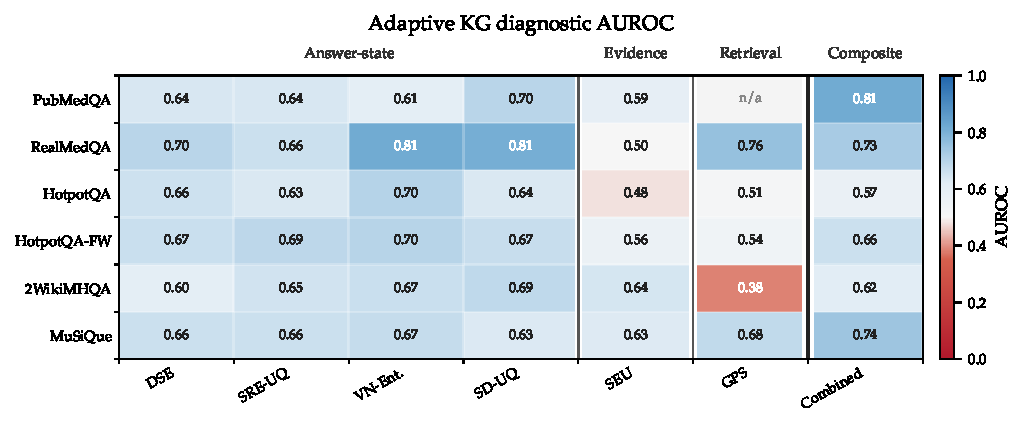
\includegraphics[width=\linewidth]{figures/adaptive_kg_auroc_heatmap}
\caption{%
  \textbf{Adaptive KG-side diagnostic AUROC across the six snapshots,
  grouped by family.}
  Incorrect answers are the positive (risk) class.
  Vertical rules separate the answer-state, evidence-state, and
  retrieval-state families; the derived Combined column is separated because
  it is not a raw metric, but the mean of within-dataset percentile ranks for
  SD-UQ, SEU, and GPS-risk.
  GPS denominators are in Appendix Table~\ref{tab:effective_denominators};
  PubMedQA is undefined because yes/no answers expose no linkable entities.
  The diverging colour scale is neutral at chance ($0.50$), red below, blue
  above.
  Cells are point estimates; bootstrap $95\%$ CIs are in Appendix
  Table~\ref{tab:headline_ci_output}.%
}
\label{fig:adaptive_kg_auroc_heatmap}
\end{figure*}

\subsection{Accuracy: Dense Retrieval Leads; Parity Is the Bar to Clear}
\label{sec:results_accuracy}

Table~\ref{tab:results_snapshot} makes the accuracy picture plain: KG-RAG
trails dense retrieval on five of the six snapshots, with $\Delta$ from
$-0.004$ (RealMedQA, effective parity) to $-0.084$ (MuSiQue), so it neither
beats nor reliably matches dense retrieval on answer quality, and
\system{} is no drop-in accuracy replacement on the harder multi-hop suites.
Where parity holds ($|\Delta| \leq 0.023$ on PubMedQA, RealMedQA, and
2WikiMultiHopQA), the diagnostic question becomes sharp: what does the graph
expose beyond passages?
The adaptive runs test whether KG-RAG preserves accuracy while exposing
anchors, paths, and provenance; the strict graph-only stress test forces
retrieval concentration to probe lock-in.

\begin{table}[t]
\centering
\small
\setlength{\tabcolsep}{6pt}
\renewcommand{\arraystretch}{1.25}
\caption{%
  \textbf{Failure taxonomy for retrieval-augmented generation.}
  Retrieval-state lock-in (top right) is the focal regime: the retrieval state
  is defective while answer-state uncertainty is low.
  Absence lock-in is flagged by retrieval-state abstention; presence lock-in,
  a coherent wrong neighbourhood, remains the hard case.
  At $N{=}5$, $42\%$ of adaptive-KG errors fall in this silent cell
  ($59\%$ dense, $84\%$ strict).%
}
\label{tab:failure_taxonomy}
\begin{tabular}{@{}l >{\raggedright\arraybackslash}p{0.30\linewidth}
                     >{\raggedright\arraybackslash}p{0.30\linewidth}@{}}
\toprule
& \textbf{Retrieval state correct}
& \textbf{Retrieval state wrong / missing} \\
\midrule
\textbf{Low answer-state}  & \cellcolor{goodgreen!15}\textbf{Certified low-risk}
                           & \cellcolor{badred!15}\textbf{Retrieval-state lock-in} \\
\textbf{uncertainty}       & \cellcolor{goodgreen!15}all three families concur
                           & \cellcolor{badred!15}answer-state silent; absence variant flagged by retrieval-state abstention, presence variant open \emph{(this paper)} \\
\addlinespace[0.3em]
\textbf{High answer-state} & \cellcolor{yellow!12}\textbf{Ordinary uncertainty}
                           & \cellcolor{black!6}\textbf{Retrieval failure} \\
\textbf{uncertainty}       & \cellcolor{yellow!12}answer-state flags it
                           & \cellcolor{black!6}answer-state flags it; retrieval-state abstains or shows no support \\
\bottomrule
\end{tabular}
\end{table}


\subsection{Silent Failures Under the Deployable Policies}
\label{sec:results_silent}

Before comparing estimators, the deployable policies already show why
answer-state uncertainty cannot be the whole story.
Table~\ref{tab:silent_failures} reports the \emph{silent-failure rate}: the
fraction of wrong answers whose answer-state uncertainty is exactly zero
(DSE $= 0$ and SD-UQ at its numerical floor), so that no score using only
within-question answer dispersion has a disagreement signal to exploit.
Requiring both conditions is deliberately conservative. DSE $=0$ is the
cluster-count view, where all samples fall in one semantic cluster. The SD-UQ
floor is the embedding-geometry view, where the geometric-mean dispersion
collapses onto the $\varepsilon = 10^{-12}$ stabiliser of
Equation~\eqref{eq:sd_uq}. A row counts as silent only when both views register
no residual variation.
The blind spot belongs to the whole family, not to one estimator: identical
samples contain no disagreement signal for DSE, SD-UQ, VN-Entropy, or any
answer-dispersion variant, though signals outside that family may still help.
Under the deployable policies, $42\%$ of adaptive KG errors and $59\%$ of
dense-retrieval errors are silent, rising to $84\%$ under the strict ablation.
Because the definition requires both semantic unanimity and the SD-UQ numerical
floor at $N=5$, these fractions are conservative symptom counts for this
answer-state family, not exact estimates of every undiagnosable error.

Confidently wrong answers are common in these deployable-policy runs, not only
in the stress regime.
Dense retrieval even produces \emph{more} silent errors than adaptive KG-RAG, so
the phenomenon is not specific to graph retrieval; nor is the dense silence a
low-budget artefact, since on dense 2WikiMultiHopQA the silent rate is still
$68\%$ at $N{=}20$.
The pattern likewise persists under relaxed silent-error floors
(Appendix~\ref{sec:appendix_silent_sensitivity}).

The KG-specific risk is \emph{auditable wrongness}: a silent error can arrive
with matched entities, typed paths, and
provenance anchors, making the system look structurally auditable while it is
wrong. Dense retrieval exposes passages, but not that symbolic trace.
As established in Section~\ref{sec:introduction}, silence is a symptom count;
route logs are needed to diagnose lock-in.

\begin{table}[t]
\centering
\footnotesize
\caption{%
  \textbf{Silent-failure rates with Wilson 95\% intervals.}
  Fraction of wrong answers with zero answer-state uncertainty
  (DSE $=0$ and SD-UQ at its numerical floor), per retrieval policy.
  $n$ is the number of wrong answered rows.%
}
\label{tab:silent_failures}
\setlength{\tabcolsep}{2.5pt}
\begin{tabular}{@{}lccc@{}}
\toprule
Dataset & Dense & Adaptive KG & Strict KG \\
\midrule
PubMedQA    & .84 [.65,.94] (25) & .67 [.48,.81] (27) & --        \\
RealMedQA   & .09 [.02,.38] (11) & .08 [.01,.35] (12) & .73 [.61,.82] (66) \\
HotpotQA    & .59 [.48,.69] (78) & .46 [.36,.56] (94) & --        \\
HotpotQA-FW & .45 [.33,.58] (58) & .18 [.11,.28] (73) & --        \\
2WikiMHQA   & .79 [.67,.87] (61) & .55 [.44,.66] (76) & .90 [.84,.94] (145)\\
MuSiQue     & .51 [.37,.65] (47) & .42 [.30,.55] (57) & --        \\
\midrule
Pooled      & .59 [.53,.65] (280) & .42 [.36,.47] (339) & .84 [.79,.89] (211) \\
\bottomrule
\end{tabular}
\end{table}

In plain terms, an answer-dispersion method cannot recover errors that never
disagree.
At the operational $N{=}5$ budget, a method that only observes sampled-answer
disagreement can recall at most $41\%$ of dense errors, $58\%$ of adaptive
KG errors, and $16\%$ of strict-stress-test errors; the remaining wrong
answers provide no within-question disagreement signal to rank.
That missing observable motivates evidence-state and retrieval-state
diagnostics.

\subsection{Answer-State Metrics Are Strong, but Not Sufficient}
\label{sec:results_output}

Given this blind spot, the next question is how much answer-state estimators
still contribute when retrieval remains adaptive.
In the adaptive runs they remain the strongest default: the AUROC heatmap
(Figure~\ref{fig:adaptive_kg_auroc_heatmap}) shows that answer-side scores have
the clearest overall association with error, especially when retrieval and
decoding still produce meaningful answer variation.
Their limit is equally clear.
When graph routing stabilises the context around a wrong entity or path, answer
disagreement can be low for incorrect answers; the score then measures the
smoothness of the answer surface rather than the reliability of the retrieved
state.
Answer-state uncertainty is therefore a strong default, but not a lock-in
diagnostic.

Within that family, the embedding-geometric scores introduced here are the best
practical answer-side baselines in these low-sample runs.
VN-Entropy and SD-UQ match or beat the imported semantic-entropy and
perturbation baselines on five of the six KG snapshots, with the exception
confined to MuSiQue; the per-dataset AUROCs and intervals are in
Appendix Table~\ref{tab:headline_ci_output}.
The stability split explains why: under high retrieval overlap, DSE falls to
chance while SD-UQ retains signal by removing the question direction before
measuring residual dispersion (Appendix
Table~\ref{tab:within_adaptive_stability}).
SD-UQ is a useful black-box baseline: cheap, embedding-only, and available
without log-probabilities, NLI calls, or model internals.

The verbalised-confidence baseline confirms the boundary rather than removing
it.
Because it asks the model for a probability, it is not blind to silent errors by
construction and recovers part of the clinical silent-error mass.
It still falls to chance on bridge-style lock-in and returns a number without
auditable provenance; the full comparison is in
Appendix~\ref{sec:appendix_verbalized}.

\subsection{The Strict Stress-Test Collapse}
\label{sec:results_collapse}

Answer-state metrics hold up under adaptive retrieval; the question is whether
they survive when retrieval is deliberately concentrated.
The sharpest stress-test signature appears in the strict graph-only regime,
where the retrieved graph state is made more concentrated by disabling dense
fallback, augmentation, reranking, and decomposition, and answer-state
uncertainty becomes a poor guide to correctness.
That answer dispersion falls under forced concentration is expected.
The informative part is what the collapse is made of, which the route
decomposition below recovers.

\begin{figure*}[t]
\centering
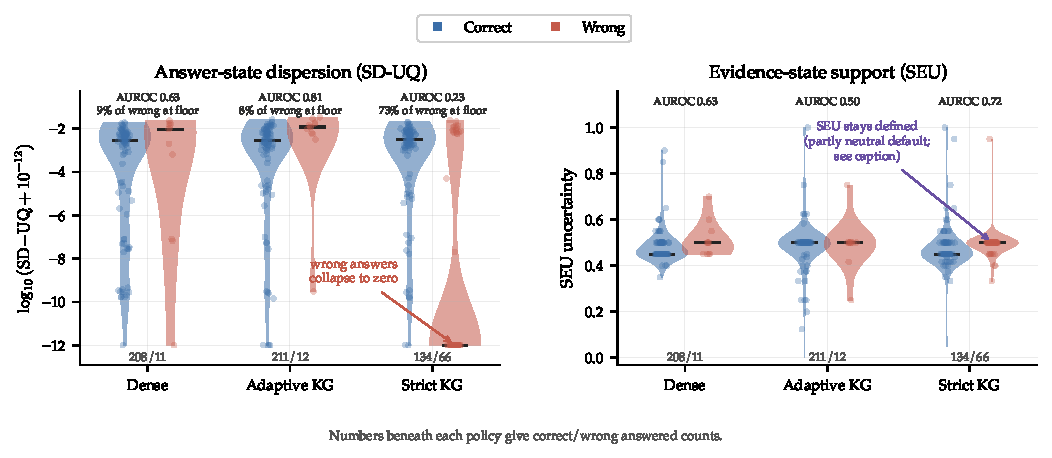
\includegraphics[width=\linewidth]{figures/context_collapse_ablation}
\caption{%
  \textbf{Context collapse in the RealMedQA strict graph-only stress test.}
  Violin/strip distributions are split by correctness, with AUROC printed in
  each panel.
  Under strict retrieval, $73\%$ of wrong answers collapse to the SD-UQ floor
  ($48/66$ vs.\ $1/12$ adaptive; Fisher exact $p = 4\times10^{-5}$).
  SEU remains separated, although Table~\ref{tab:silent_accounting} shows that
  much of the strict signal comes from empty-retrieval defaults.
  The counts beneath each policy are correct/wrong answered rows.
  Strict graph-only retrieval is a mechanism probe.%
}
\label{fig:context_collapse_ablation}
\end{figure*}

\begin{figure*}[t]
\centering
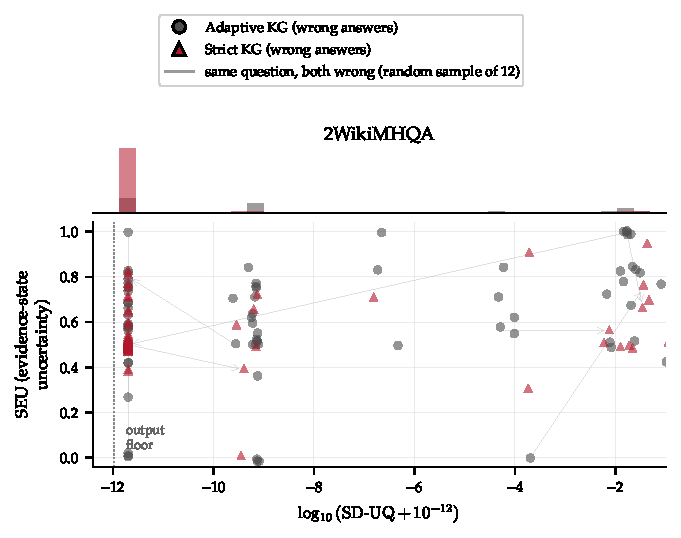
\includegraphics[width=0.92\linewidth]{figures/lockin_migration}
\caption{%
  \textbf{Lock-in as migration into the low-dispersion corner
  (2WikiMultiHopQA).}
  Each point is a \emph{wrong} KG answer, plotted by answer-state dispersion
  (SD-UQ, log scale) and evidence-state uncertainty (SEU), under the
  adaptive policy (grey circles) and the strict graph-only stress test
  (red triangles).
  Grey arrows connect a uniformly random sample of $12$ questions that are
  wrong under \emph{both} policies.
  Under strict retrieval the SD-UQ mass collapses onto the floor while SEU
  remains spread.
  Small vertical jitter is added for legibility.%
}
\label{fig:lockin_migration}
\end{figure*}

Across all paired adaptive--strict questions, $43/196$ RealMedQA questions and
$87/242$ 2WikiMultiHopQA questions move from correct under adaptive KG to
wrong-and-silent under the strict graph-only stress test.
Among questions already wrong but not silent under adaptive KG, another
$2$ RealMedQA and $12$ 2WikiMultiHopQA questions become wrong-and-silent
under strict retrieval; on 2WikiMultiHopQA, $31$ questions remain
wrong-and-silent under both policies.
Thus the stress test does not merely lower accuracy: it moves errors into the
part of the state space where answer-dispersion methods have no disagreement
signal to exploit.

A strict RealMedQA stress test makes the lock-in regime visible directly on the
cleanest parity dataset. As scoped in Section~\ref{sec:introduction}, it is a regime probe:
it shows that lock-in can arise and what the silent signature looks like. The
adaptive rates in Section~\ref{sec:results_silent} measure the deployable-policy
footprint.
It is deliberately harsher: clean KG accuracy falls to $0.670$ on $200$
answered questions, and average within-question chunk overlap rises from
$0.558$ to $0.661$ (Appendix Table~\ref{tab:retrieval_overlap}).
The danger is stability around a wrong symbolic state, not retrieval stability
in itself.
Under that concentrated regime, answer-state ranking largely collapses, as the
strict/adaptive comparison in Figure~\ref{fig:context_collapse_ablation} shows:
DSE AUROC is $0.463$, VN-Entropy AUROC is $0.248$, and SD-UQ AUROC is $0.233$.
On the question subset shared by the two policies, the adaptive-to-strict
SD-UQ gap is $+0.52$ AUROC (paired-bootstrap 95\%~CI $[0.28, 0.73]$,
$n=196$).
The migration plot in Figure~\ref{fig:lockin_migration} shows the mechanism at
question level:
wrong answers migrate from moderate output dispersion under the adaptive
policy into a dense column at the SD-UQ floor under strict retrieval, while
their evidence-support scores remain spread.
That matters because the low-dispersion corner is exactly where answer-state
confidence looks most reassuring and is least informative.
By contrast, SEU reaches $0.721$ AUROC, and GPS reaches $0.746$ on $142/200$
non-abstained rows (Appendix Table~\ref{tab:realmedqa_strict_entity}): the
answer surface goes silent while retrieval-facing scores still rank errors
(GPS here is in its calibration domain).
The contrast holds under an independent Llama-3.3-70B judge ($95.0\%$
agreement, $\kappa = 0.89$): SD-UQ stays collapsed while SEU and GPS still rank
the errors, which same-model self-preference would not explain
(Section~\ref{sec:limitations}).

\paragraph{Route decomposition.}
First, the collapse is not a chunk-level artefact.
An interventional dose-response reduces chunk overlap from $0.67$ to $0.29$,
but leaves SD-UQ AUROC flat ($0.18$) and the silent-error count unchanged
(Appendix~\ref{sec:appendix_doseresponse}).

Second, route logging shows where the silent state lives.
Every silent error in the strict clinical run is an empty-retrieval row
($48/48$ at $n=230$).
Strict anchoring found no usable context, the same empty state recurred across
all five samples, and the generator answered unanimously from parametric
memory.
This points first to removed fallback and vector augmentation as proximate
contributors in this stress run, but the design still changes multiple
components and does not isolate one as the cause.
On the populated-route rows, answer-state ranking is healthy (SD-UQ AUROC
$0.79$).
Much of SEU's apparent survival is mechanical: empty-retrieval wrong rows
receive the all-neutral default $0.5$, which ranks above confidently supported
correct rows; populated-row SEU is only $0.56$.
This is \emph{absence} lock-in, whose simplest reliable flag is the
empty-route/abstention observable, not answer dispersion or evidence
entailment.

Third, the strict 2WikiMultiHopQA run decomposes the same way but leaves a
remainder: $110$ of $130$ silent errors are empty-retrieval, while $20$ ride
populated entity-first routes, wrong-but-coherent neighbourhoods of the
Osireion type (\emph{presence} lock-in), and populated-row SD-UQ stays
degraded there ($0.65$).
Presence lock-in is the harder case: the answer surface and the route
observable are both silent, leaving only evidence-level checks.
It is also a setting where SEU itself proved unreliable (the strict 2-hop
slice), which is why the composite recommendation does not reduce to any single
surviving family.

Under the deployable adaptive policy the silent errors are
mostly presence-like: of the $141$ pooled adaptive silent errors, $99$ carry
recorded route metadata, and among those $89$ ride populated iterative
multi-hop routes with none on the empty-retrieval route, so the
deployable-policy footprint is not an empty-retrieval artefact.
The route claim is limited to the logged subset: the remaining $42$ silent
errors lack route metadata, so their absence/presence mix is not recoverable
from the saved logs.
Decomposing those $141$ adaptive silent errors by which family flags them:
$67$ carry an evidence-state contradiction ($\mathrm{SEU}>0.5$), $127$ carry
weak or absent graph support (GPS $>0.5$ or abstention), and only $7$
($5\%$) remain unflagged by every non-answer family.
A manual audit of these seven (Appendix~\ref{sec:appendix_residue}) finds
mostly benchmark-ambiguous questions, wrong-answer-slot errors, and parametric
conflations rather than confirmable deep presence lock-in whose evidence
\emph{entails} the wrong answer (the Baltic Cup type of
Table~\ref{tab:lockin_gallery}); since retrieved chunk texts are not archived,
that deceptive type cannot be confirmed from logs.

Flagging the cases where all three families fail, with SEU and GPS both near
zero on a wrong answer, would need exactly what the logs lack here: archived
chunk text for cross-passage contradiction mining, and relation-level path
faithfulness to check that the connecting path uses the relation the question
asked for rather than a locally coherent but wrong one.
Both are concrete, retrieval-replay-only extensions, not new theory.
Table~\ref{tab:silent_accounting} makes the accounting explicit.

\begin{table*}[t]
\centering
\scriptsize
\caption{%
  \textbf{Silent-error accounting from saved logs.}
  Buckets are mutually exclusive and apply only to wrong answered rows.
  ``Max answer recall'' is the structural upper bound for any
  answer-dispersion-only detector at the $N{=}5$ budget: silent wrong answers
  contain no sampled-answer disagreement signal.
  Empty denotes absence lock-in; Pop.+SEU and Pop.+GPS are populated-route
  silent errors flagged by evidence or graph-support signals.
  Unflagged is the residue with no non-answer-family flag.%
}
\label{tab:silent_accounting}
\setlength{\tabcolsep}{3pt}
\begin{tabular}{@{}lrrrrrrrr@{}}
\toprule
Run & Wrong & Silent & Max answer recall & Empty & Pop.+SEU & Pop.+GPS & Route-unk.+flag & Unflagged \\
\midrule
Adaptive KG pooled & 339 & 141 & .58 & 0 & 40 & 44 & 50 & 7 \\
Strict KG pooled   & 211 & 178 & .16 & 158 & 13 & 6 & 0 & 1 \\
RealMedQA strict   & 66  & 48  & .27 & 48  & 0  & 0 & 0 & 0 \\
2WikiMHQA strict   & 145 & 130 & .10 & 110 & 13 & 6 & 0 & 1 \\
\bottomrule
\end{tabular}
\end{table*}
Under this deterministic graph-only regime, answer-surface uncertainty can
cease to track correctness.
Which signal survives depends on the variant: route or abstention observables
for absence, and evidence-level checks, imperfectly, for presence.

The same pattern appears on the newer 2WikiMultiHopQA $n=250$ run when the
three retrieval policies are compared on the identical question subset; the
full hop-stratified breakdown is in Appendix
Table~\ref{tab:twowiki_hopwise_diagnostics}.
The adaptive KG policy is the appropriate deployment comparison: it remains
close to dense retrieval overall (clean accuracy $0.689$ versus $0.712$) and
matches dense retrieval on the 4-hop slice.
On the 4-hop slice, strict graph-only KG has zero clean accuracy while
SD-UQ and VN-Entropy both collapse essentially to zero: the answer surface is
stable precisely when the retrieved graph state has become wrong enough to
make every answer fail.
Low answer-state uncertainty is not intrinsically bad. In the dense 4-hop row,
SD-UQ is also near zero, but VN-Entropy remains non-zero and clean accuracy
stays high, so the collapse signature is the joint collapse of SD-UQ and
VN-Entropy together with failed answers, not low SD-UQ alone.
For KG-RAG, answer agreement must therefore be read alongside evidence- and
retrieval-state diagnostics when the symbolic state has concentrated around a
wrong neighbourhood.
Per-question support comes from a dedicated graph-state diversity run on
HotpotQA-FullWiki that logged per-sample overlap for the seed entities, paths,
subgraph, and chunks ($n=221$ answered, $74$ wrong; Table~\ref{tab:diversity_run}).
Across the $N=5$ samples the retrieval state is highly stable
(seed-entity Jaccard $0.99$; path, subgraph, and chunk $0.58$--$0.65$), so
repeated samples really do condition on nearly the same state; and among
\emph{wrong} answers more overlap predicts lower dispersion
(path/subgraph/chunk Spearman $\rho = -0.30$/$-0.23$/$-0.24$, all $p<0.05$,
$n=74$; the seed-entity coupling is null only because seed overlap saturates
near $1.0$, leaving no variance to correlate against).
The archived traces show the same sign, carried by the bridge-style
2WikiMultiHopQA trace ($\rho = -0.32$, $p = 0.01$, $n = 60$; pooled
$\rho = -0.27$), with no comparable pattern on the dense side.
These analyses support the mechanism without identifying it causally
(Appendix~\ref{sec:appendix_diversity}, \ref{sec:appendix_concentration};
the per-dataset concentration facets are in Figure~\ref{fig:concentration_facets}).

\begin{table}[t]
\centering
\scriptsize
\caption{%
  \textbf{Per-sample graph-state diversity on the dedicated HotpotQA-FullWiki
  run} ($n=221$ answered, $74$ wrong).
  \emph{Stability} is the mean (median) pairwise Jaccard overlap across the
  $N=5$ samples per question, by retrieval-state family.
  \emph{Coupling} is the correlation between that per-question overlap
  and answer-state dispersion (SD-UQ) among wrong answers ($n=74$), reported as
  Spearman's $\rho$ with its two-sided $p$-value; a negative
  value means more overlap goes with less dispersion, the lock-in prediction.%
}
\label{tab:diversity_run}
\begin{tabular}{@{}lcccc@{}}
\toprule
 & \multicolumn{2}{c}{Stability (Jaccard)} & \multicolumn{2}{c}{Coupling vs SD-UQ} \\
\cmidrule(lr){2-3}\cmidrule(lr){4-5}
Family & Mean & Median & $\rho$ & $p$ \\
\midrule
Seed entity & $0.99$ & $1.00$ & $+0.09$ & $0.47$ \\
Path        & $0.58$ & $0.58$ & $-0.30$ & $0.009$ \\
Subgraph    & $0.64$ & $0.63$ & $-0.23$ & $0.048$ \\
Chunk       & $0.65$ & $0.65$ & $-0.24$ & $0.037$ \\
\bottomrule
\end{tabular}
\end{table}

HotpotQA supplies a useful counterweight.
Dense retrieval leads on accuracy ($0.655$ vs.\ $0.605$; FullWiki $0.721$ vs.\
$0.665$) while answer-state AUROCs stay healthy on both systems and GPS is only
weakly discriminative ($0.51$ and $0.54$ usable-row AUROC; Appendix
Table~\ref{tab:hotpot_fullwiki_stress}).
These runs mark the thesis boundary rather than contradicting it: when dense
retrieval already has a compact, well-indexed candidate set, graph
organisation adds provenance and traceability but the current policy does not
improve answer quality or retrieval-state ranking.

Figure~\ref{fig:selective_prediction} reframes the same results as a
selective-prediction problem, the clinical form of the uncertainty question:
if a diagnostic score is high, should the system answer, broaden retrieval,
or send the case to review?
In ordinary adaptive runs, answer-side scores often give the cleanest
rejection signal.
In lock-in regimes, SEU and GPS have to be read as provenance checks rather
than weaker versions of answer-state entropy.

The key appendix row is the strict graph-only 4-hop slice
($n=58$, clean accuracy $0.000$, SD-UQ mean $0.000$, VN-Entropy mean $0.000$).
AUROC is intentionally left undefined because all 58 clean answers are
incorrect, so the evidence is the conjunction of zero accuracy and collapsed
output scores, not a forced ROC statistic: a mechanism demonstration, not a
deployment result.

\subsection{Evidence-State Metrics Add Support-Level Signal}
\label{sec:results_grounding}

If the answer surface goes silent under concentration, the next
question is whether the retrieved evidence itself betrays the error.
Evidence-state measures ask whether the retrieved passages support the answer
that was produced, not whether sampled answers agree; this matters especially
in high-accuracy or near-parity settings where the deployment question is
whether the answer can be justified by retrieved evidence.

The aggregate evidence-state signal is weaker than the answer-state family as
a global ranker, but complementary rather than redundant.
SEU's survival under lock-in is dataset-dependent. It reaches $0.721$
AUROC on the strict RealMedQA ablation, although the route decomposition in
Section~\ref{sec:results_collapse} shows that much of this signal comes from
the all-neutral default over empty-retrieval rows, not from genuine entailment.
On the strict 2WikiMultiHopQA 2-hop slice, it falls below chance
(Appendix Table~\ref{tab:twowiki_hopwise_diagnostics}). Evidence support is
therefore useful, but not uniformly robust to retrieval concentration.
The 2-hop failure has a concrete mechanism: on bridge questions the strict
policy retrieves passages about the wrong-but-coherent anchor, and those
passages weakly \emph{entail} the wrong answer drawn from that neighbourhood
rather than contradicting it, so low SEU and incorrectness coincide.
On the clinical corpus, the contradiction is visible in the retrieved text
itself; SEU survives there for this reason.
SEU is also low-resolution where retrieval returns long, loosely-relevant
chunks: on the adaptive RealMedQA run, $74\%$ of answered rows receive the
all-neutral value $0.5$ because no retrieved chunk is judged to entail or
contradict the answer, which explains the chance-level adaptive AUROC there.
In that regime the score is silent rather than wrong; sentence-level
entailment scoring is the plausible refinement, but it requires re-running
retrieval rather than replaying logs.
The selective-prediction curves in Figure~\ref{fig:selective_prediction}
and the fixed-coverage operating points in Appendix
Table~\ref{tab:operating_points} give the same lesson in decision form.

\begin{figure*}[t]
\centering
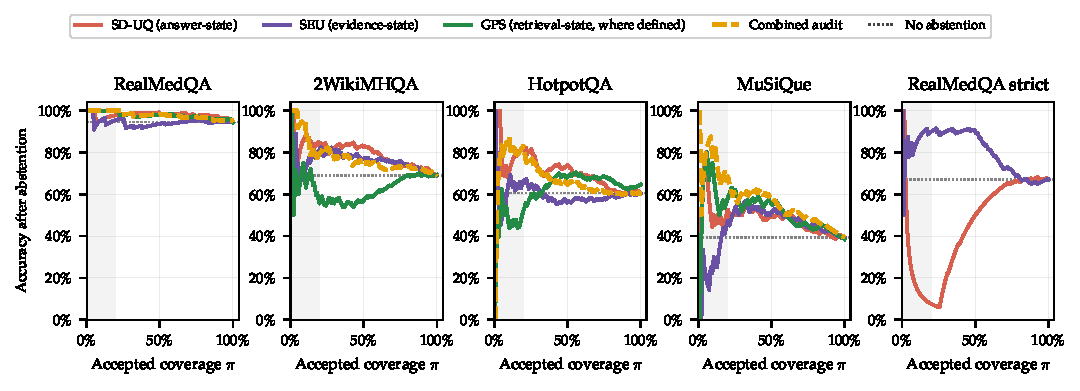
\includegraphics[width=\linewidth]{figures/coverage_accuracy}
\caption{%
  \textbf{Selective prediction with different KG-side diagnostic families},
  including the RealMedQA strict ablation (rightmost panel).
  Curves sort answered KG-RAG queries by increasing uncertainty and then
  report the accuracy retained at each accepted coverage level; the dotted
  line is the no-abstention accuracy and the shaded band marks the noisy
  $<20\%$-coverage region.
  The strict panel carries the decision-form headline: SD-UQ gating
  \emph{inverts}: accepting the lowest-dispersion answers first means
  accepting the silent wrong mass, while SEU gating climbs toward $90\%$.
  GPS and the combined audit are omitted from the strict panel because GPS
  comes from post-hoc replay rather than row-level logs.%
}
\label{fig:selective_prediction}
\end{figure*}
Under the adaptive policy, gating on SD-UQ alone is the strongest simple
abstention rule; under the strict clinical ablation that rule becomes
uninformative ($0.338$ error at $80\%$ coverage against a $0.330$
no-abstention base) while SEU gating cuts the residual error to $0.269$, an
$18\%$ relative reduction in the regime where the answer surface is silent.
The useful diagnostic changes with the retrieval regime; a single global
ranking hides that switch.

\subsection{Where Retrieval-State Diagnostics Work and Where They Do Not}
\label{sec:results_structural}

Retrieval-state diagnostics ask the complementary question: when does the graph
state itself reveal weak support?
GPS behaviour is domain-dependent.
On the clinical shared-corpus setting where its two hyperparameters were
calibrated, it is a useful error ranker ($0.76$ adaptive, $0.75$
strict); on the held-out open-domain suites transfer is uneven (MuSiQue $0.68$
with per-question depth, but HotpotQA $0.51$, FullWiki $0.54$, and
2WikiMultiHopQA $0.38$ near or below chance).
A sensitivity replay over $\tau\in\{0.50,\ldots,0.70\}$ and
$\gamma\in\{0.2,\ldots,1.0\}$ leaves the held-out open-domain GPS AUROCs
essentially unchanged (SD $\leq 0.018$ for HotpotQA, FullWiki,
2WikiMultiHopQA, and MuSiQue; Appendix Table~\ref{tab:gps_sensitivity}), so
the weak 2WikiMultiHopQA ranking is not a threshold/decay artefact.
GPS scores graph support for the generated answer, not correctness.
It can therefore rate a wrong-but-coherent neighbourhood as low risk: in the
Baltic Cup case of Table~\ref{tab:lockin_gallery}, the wrong entity is reachable,
GPS is $0.00$, SEU is $0.00$, and the answer surface has near-zero dispersion.
The decomposition makes that failure visible but does not solve it.
Retrieval-state AUROC is therefore computed only on rows with linkable answer
entities, with linking failures reported as abstentions
(Table~\ref{tab:results_snapshot}). GPS contributes most reliably as an
abstention record, usable denominator, and trace-level support check; its scalar
ranking is useful only in validated domains.
A fixed-bin reliability check makes the same point without AUROC:
RealMedQA error rates rise from $0/39$ in the lowest GPS-risk bin to $6/42$
in the highest, but the open-domain bins are not monotone, especially on
2WikiMultiHopQA (Appendix Table~\ref{tab:gps_reliability_bins}).

Soft answer-entity linking substantially reduces the abstention cost: usable
denominators now cover most answered rows (e.g.\ $185/218$ on HotpotQA
FullWiki, up from $69$ under pure surface matching), with the per-dataset
values in Table~\ref{tab:results_snapshot} and Appendix
Table~\ref{tab:effective_denominators}.
PubMedQA still abstains completely because binary answers expose no answer
entities, a structural boundary rather than a linking failure.
Coverage repair is not ranking repair: the held-out AUROCs above
show that making more rows scoreable does not by itself make the score a
better error ranker.
Closing the open-domain ranking gap most plausibly requires relation-level
path faithfulness, checking that the connecting path uses the relation the
question asked for, rather than further entity-linking improvements.
The 2WikiMultiHopQA replay shows the problem directly.
The adaptive $n=250$ run gives GPS AUROC $0.38$ on $182/244$ usable rows because
$71\%$ of correct adaptive answers have their gold entity unreachable in the
retrieved subgraph, against $45\%$ of wrong ones.
Here GPS is not miscalibrated; it is exposing a retrieval policy that can make
the wrong answer reachable while leaving the gold answer outside the graph state.

The post-hoc replay on the full $n=230$ answer log, recomputing only
GPS, without rerunning generation or
retrieval, raises KG-side coverage from $97/223$ to $195/223$ and AUROC from
$0.47$ to $0.76$ (Appendix Table~\ref{tab:realmedqa_replay}); the same replay
reaches $0.89$ on the dense side.
RealMedQA is the calibrated case: it shows what retrieval-state scoring can
deliver on a clinical shared corpus, while the held-out rows above show the
generalisation limit.

\subsection{Concrete Cases}
\label{sec:results_cases}

The aggregate AUROCs and route statistics summarise behaviour across
questions; the Osireion trace in Figure~\ref{fig:lockin_trace} shows
how the three families interact on a single answer, and is deliberately not a
case where every diagnostic succeeds.
Answer-state uncertainty is at its floor ($\mathrm{DSE}=0$,
$\mathrm{SD\text{-}UQ}\approx 0$) because all samples repeat the wrong entity;
GPS is low ($0.44$), so it does not flag the case: the wrong entity is
reachable in the retrieved graph. This is correct behaviour for a
risk-oriented support diagnostic, but not a truth guarantee. SEU alone raises
risk ($1.0$), because every retrieved chunk
contradicts the confident, graph-coherent answer.
The practical meaning of path faithfulness is therefore that the graph can make
a wrong reasoning chain visible even when the scalar retrieval-state score
reports low risk, provided the evidence-support head is read with it; the full
per-case audit readout is in Appendix Table~\ref{tab:path_faithfulness_case}.
A consolidated case gallery, with seven verified lock-in failures, four KG
successes, and per-case diagnostic readouts, is in
Appendix~\ref{sec:appendix_cases} (Table~\ref{tab:lockin_gallery}).

\subsection{The Composite-Suite Thesis}
\label{sec:results_composite}

Finally, if the three families answer different diagnostic questions, the
decision layer should not collapse them too early.
They also barely move together, which is the quantitative case
for keeping them apart; Appendix Figure~\ref{fig:family_disagreement} shows this
for the adaptive KG setting.
Across the six-snapshot heatmap suite ($n=803$ pooled non-abstained KG rows),
the pooled KG-side Spearman correlations are small to modest:
$\rho=0.03$ for SD-UQ versus SEU, $\rho=-0.27$ for SD-UQ versus GPS, and
$\rho=-0.10$ for SEU versus GPS; the pooled family-disagreement scatter is in
Appendix Figure~\ref{fig:family_disagreement}.
The three scores therefore carry partly separate diagnostic signal, even if low
correlation alone cannot identify distinct latent causes.
Because GPS is a graph-support diagnostic reported in risk orientation rather
than an information-theoretic uncertainty score, lower GPS means stronger local
graph support for the generated answer, so the negative SD-UQ--GPS sign should
not be read as a universal risk law.

If all three families tracked the same object, a single scalar confidence
score would suffice; they do not, and expose different failure modes.
The recommendation is a composite diagnostic suite, not a single-metric
leaderboard. In practice, a low answer-state score should not override a
retrieval-state abstention, a fragile graph path, or high evidence
contradiction; such discordant profiles are good candidates for abstention,
broader retrieval, or human review.
A deliberately simple percentile-rank audit score, averaging SD-UQ, SEU, and
GPS-risk within each dataset, shows how the three families can feed a decision
layer. It is uneven, but useful where answer dispersion is coarse
(e.g.\ PubMedQA Combined $0.813$ vs.\ SD-UQ $0.699$;
Appendix~\ref{sec:appendix_composite},
Table~\ref{tab:composite_audit_score}).

\paragraph{A conjunctive low-risk audit rule.}
The conservative rule is narrow by design: it selects $7.7\%$ of answers at
$91.9\%$ accuracy ($86$ of $1{,}117$ questions), against a $69.7\%$ base rate.
It treats a response as low-risk only when all three families concur: low
answer-state uncertainty (SD-UQ in the lower half of its dataset
distribution), non-contradictory evidence support ($\mathrm{SEU} \leq 0.5$),
and defined, present retrieval-state support ($\mathrm{GPS} \leq 0.5$).
The cutoffs are label-free: SEU and GPS use their fixed neutral point ($0.5$),
and SD-UQ uses the dataset median. A deployment would choose its own coverage
point on held-out calibration data.
On the clinical target domain it selects $22\%$ of answers at $100\%$ precision
under the automated judge ($48/48$ correct), a figure that would need
human-expert confirmation before any clinical use (Section~\ref{sec:ethics}).
The same fixed policy is applied unchanged to every dataset. Table~\ref{tab:certificate_perds}
therefore acts as the cross-dataset generalisation view: it reports
per-dataset coverage, precision with Wilson intervals, and recall. Recall is
included because a high-precision selection rule is trivial without it.
Coverage is structurally limited: the rule cannot select answers
with no linkable answer entity (binary, numeric, or label-space answers, where
GPS abstains by construction), so on those formats it defers rather than
selects, and a deployment would need a separate fallback.
The conjunction beats matched-coverage scalar gates: SD-UQ alone gives
$81.4\%$ precision at the same coverage, and the percentile-rank combined score
gives $88.4\%$. A dataset-stratified Mantel--Haenszel check gives the same
direction (odds ratio $3.39$, bootstrap 95\% CI $[1.64, 10.99]$;
Appendix~\ref{sec:appendix_reproducibility}).
The rule is exploratory and domain-conditional. It is strongest on the clinical
target domain, thin-coverage on the harder multi-hop sets, and undefined for
label-space answers. Its purpose is to show what the three-family decomposition
makes possible as an audit policy.

\begin{table}[t]
\centering
\scriptsize
\caption{%
  Per-dataset conjunctive audit-rule behaviour on the adaptive KG runs.
  Recall is the fraction of all \emph{correct} answers selected by the rule;
  it is high-precision and low-recall by design,
  Wilson intervals expose the small denominators,
  and its utility presumes that unselected answers are routed to ordinary
  confidence handling or review rather than discarded.%
}
\label{tab:certificate_perds}
\setlength{\tabcolsep}{2.5pt}
\begin{tabular}{@{}lrrcr@{}}
\toprule
Dataset & Selected & Prec. & 95\% CI & Recall \\
\midrule
PubMedQA & 0/100 (0\%) & -- & -- & 0.00 \\
RealMedQA & 48/223 (22\%) & 1.000 & [0.926, 1.000] & 0.23 \\
HotpotQA & 6/238 (3\%) & 0.833 & [0.436, 0.970] & 0.04 \\
HotpotQA-FW & 26/218 (12\%) & 0.808 & [0.621, 0.915] & 0.14 \\
2WikiMHQA & 4/244 (2\%) & 1.000 & [0.510, 1.000] & 0.02 \\
MuSiQue & 2/94 (2\%) & 0.500 & [0.095, 0.905] & 0.03 \\
\midrule
Pooled & 86/1117 (7.7\%) & 0.919 & [0.841, 0.960] & 0.10 \\
\bottomrule
\end{tabular}
\end{table}
The only data-dependent threshold (the per-dataset SD-UQ median)
survives held-out evaluation: computing it on a random half of each dataset
and applying the rule to the other half gives $91.8\%$ mean precision
(5th--95th percentile $86.7$--$97.4\%$ over $200$ splits) at unchanged
coverage, so the in-sample number is not threshold overfitting.
Per-dataset behaviour exposes both cautionary cases: 2WikiMultiHopQA
selects only four answers ($2\%$ coverage) despite weak GPS ranking, while
MuSiQue selects two answers at only $50\%$ precision.
Per-domain validation is mandatory.
Coverage is bounded mainly by GPS definability and SEU neutrality, so
the refinements above (soft linking already; sentence-level entailment next)
are the most direct route to higher audit-rule coverage.
A simple learned alternative does not transfer better in this fixed-subset test:
leave-one-dataset-out logistic gating selects $7.5\%$ of answers at $85.7\%$
precision. With three scalar features and substantial cross-dataset shift,
conjunctive gating remains the more auditable policy.

\section{Conclusion}
\label{sec:conclusion}

Retrieval-state lock-in turns agreement into the wrong kind of reassurance.
When the retriever repeatedly returns the same empty or wrong state, more
samples need not test more possibilities; they may simply repeat the same
condition. The confidence question therefore changes. It is not only whether
the answer is stable, but which object is stable: the answer surface, the
retrieved evidence, or the retrieval state itself.

The experiments show that answer-state uncertainty remains a useful default,
but a bounded one. In the deployable-policy runs, $42$--$59\%$ of errors already
have zero observed answer dispersion at $N{=}5$, so an answer-only method has no
within-question disagreement signal to recover. Evidence-state diagnostics can
catch some of these failures by testing support in the retrieved text. GPS adds
a narrower graph-support view, strongest on the calibrated clinical corpus and
weak on several open-domain multi-hop suites. The field-level lesson is simple:
agreement, support, and retrieval grounding are different observables, and a
single confidence scalar hides that difference.

The practical recommendation is correspondingly conservative. Report answer-,
evidence-, and retrieval-state signals separately, and call an answer low-risk
only when all three agree: low answer uncertainty, adequate evidence support,
and present graph support. In \system{}, this conjunctive rule selects a small
subset at $91.9\%$ pooled accuracy against a $69.7\%$ base rate, and reaches
$100\%$ precision under the automated judge on the clinical target domain at
$22\%$ coverage, pending human-expert confirmation before any clinical use.
Unselected answers are not thereby wrong; they are simply not low-risk by this
audit.

The unresolved case is presence lock-in: the system retrieves a coherent but
wrong neighbourhood, and the answer is locally supported by that state.
That is the setting where relation-level path faithfulness matters most:
future systems should test not only whether an answer entity is reachable, but
whether the path uses the relation the question actually asks for. The same
diagnostic decomposition also suggests a control policy. When answer samples
agree but evidence- or retrieval-state diagnostics disagree, the retriever
should test a nearby alternative state, for example by masking the dominant
intermediate anchor while preserving the seed entities. If the answer changes,
it was anchored to that state; if it does not, the evidence was stable across
the tested perturbation.

\subsection{Limitations}
\label{sec:limitations}

The strict graph-only setting is a mechanism probe, not a deployable policy or
a one-component ablation. It changes fusion, reranking, decomposition, and
fallback together, so it demonstrates a regime in which answer-state uncertainty
fails rather than estimating production prevalence. The route logs make removed
fallback and vector augmentation the most plausible contributors in the strict
clinical collapse, but a factorial ablation would be needed to apportion the
effect.

GPS is a graph-support score in risk orientation: lower values mean stronger
support for the generated answer, not greater correctness. It is strongest on
the calibrated clinical corpus and weak on several open-domain multi-hop suites
despite the sensitivity replay in Appendix~\ref{sec:appendix_gps_sensitivity}.
Yes/no and other label-space answers remain outside its design.
The retrieval-state family is therefore justified as an observable class
(anchors, paths, subgraphs, and routes), while GPS is only one conditional scalar
instantiation of that class.

SEU is also local: it tests answer--evidence consistency, not whether the model
used the evidence. Its neutral plateau can make empty-context failures easier to
rank than populated presence-lock-in failures, where the wrong neighbourhood may
locally support the wrong answer.

The empirical scale supports the central contrasts but not fine leaderboard
claims between neighbouring metrics. Correctness labels come from an automated
semantic judge and survive an independent Llama-family re-judge, but human or
domain-expert adjudication would be needed before treating silent errors as
clinical risk. The experiments also use a single generation model
(GPT-4o-mini), and fine-grained retrieval-state diversity is logged only in the
dedicated diversity run.
The paper should therefore be read as a diagnostic methodology and fixed-system
empirical audit, not as a cross-model survey of lock-in prevalence.

The retrieval-state diagnostics are graph-native. The silent-error phenomenon
is not: dense retrieval shows it too. Extending the same decomposition to
dense-RAG retrieval states, for example through citation-path or passage-link
plausibility, is the most direct route to broader generality.

\subsection{Ethical and Safety Considerations}
\label{sec:ethics}

Nothing in these results licenses autonomous clinical answering. The
audit rule is deliberately high precision and low coverage; the unselected
majority should be routed to ordinary confidence handling, broader retrieval,
or human review. Lock-in also has an adversarial analogue: a corpus or query
can be shaped to anchor retrieval in a plausible but wrong neighbourhood.
Retrieval diversity constraints and anchor-masking controls are plausible
defences, but they remain future work.
Adversarial robustness lies outside this evaluation. The diagnostic
decomposition is still a prerequisite for it: a failure mode that cannot be
observed cannot be defended against.


\bibliographystyle{plainnat}
\bibliography{references}

\appendix
\onecolumn
% =============================================================================
\section{Residual-Mass Bound for Stabilised Retrieval}
\label{sec:appendix_residual_bound}

The collapsed-context approximation in Section~\ref{sec:background} can be
read as a simple mixture argument.
Let $\alpha = p(c^\star \mid q)$ and define the residual context mixture
\[
  \pi_{\mathrm{res}}(r)
  =
  \frac{1}{1-\alpha}
  \sum_{c \in \mathcal{C}(q)\setminus\{c^\star\}}
  p(r \mid q,c)\,p(c\mid q),
\]
whenever $\alpha < 1$.
Then
\[
  p(r\mid q)
  =
  \alpha\,p(r\mid q,c^\star)
  +
  (1-\alpha)\,\pi_{\mathrm{res}}(r),
\]
and therefore
\[
  \bigl\|p(r\mid q)-p(r\mid q,c^\star)\bigr\|_{\mathrm{TV}}
  =
  (1-\alpha)
  \bigl\|\pi_{\mathrm{res}}(r)-p(r\mid q,c^\star)\bigr\|_{\mathrm{TV}}
  \leq 1-\alpha.
\]
The bound is not used as an estimator in the experiments.
It only states the condition under which the stylised approximation is
meaningful: the residual routing mass must be small.

% =============================================================================
\section{KG Construction and System Configuration}
\label{sec:appendix_construction}

\subsection{Knowledge Graph Construction Pipeline}
\label{sec:appendix_kg}

This section documents the full construction pipeline for reproducibility.
The key design choice is that the KG is built passage-wise with chunk-level
provenance, so every triple and path traces back to the text that licensed it.

\paragraph{Text chunking.}
Input documents are split into overlapping passages using a token-aware
recursive splitter (tiktoken-based, with a character-based fallback when the
tokenizer is unavailable) with chunk size $L = 1{,}500$ tokens and overlap
$\delta = 200$ tokens.
Each chunk receives an embedding at construction time using
\texttt{all-MiniLM-L6-v2} (384 dimensions) from Sentence Transformers
\citep{reimers2019sentencebert}.
Chunks are stored as \textsc{Chunk} nodes in Neo4j with a SHA-1 content
hash as identifier and a \textsc{Part\_Of} edge to their parent
\textsc{Document} node.

\paragraph{Entity and relation extraction.}
Entities and typed relations are extracted from each chunk via a prompted
LLM call (GPT-4o-mini; \citealp{openai2024gpt4omini}).
The LLM is prompted to return a JSON object with an \texttt{entities}
array and a \texttt{relationships} array.
Each entity has fields \texttt{id}, \texttt{type}, \texttt{name}, and
\texttt{description}; each relation has \texttt{source}, \texttt{target},
\texttt{type}, and \texttt{description}.
Two extraction modes are supported:

\begin{enumerate}
  \item \textbf{Ontology-guided extraction.} When a domain type schema is
    provided, it is first parsed from JSON or OWL/RDF into a single typed
    internal representation.
    The extraction prompt then includes ontology entity types with
    descriptions and typed properties, together with relationship types and
    their domain/range/cardinality constraints.
    After extraction, entity types are normalised with ontology guidance via
    embedding-based cosine similarity against ontology class labels
    (threshold $\tau = 0.50$), with exact substring matching and keyword
    heuristics as fallback.
    Relationship labels are then canonicalised to the closest
    schema-compatible relationship type using domain/range compatibility and
    fuzzy matching when needed.
    In the biomedical and clinical experiments, types include
    \textsc{Disease}, \textsc{Treatment}, \textsc{Symptom},
    \textsc{Biomarker}, and \textsc{Anatomy}.

  \item \textbf{Open extraction.} Without a type schema, the LLM extracts
    entities and relations freely.
    Used for the open-domain datasets (HotpotQA, HotpotQA FullWiki,
    2WikiMultiHopQA, and MuSiQue).
\end{enumerate}

The important point is that the current system does \emph{not} induce or
generate an ontology from the document collection.
It loads a user-provided ontology/schema and uses it to guide extraction,
typing, and relationship normalisation during KG construction.

\paragraph{Neo4j schema.}
Entities are stored as \textsc{Entity} nodes with compound labels
\texttt{:\_\_Entity\_\_:Type} (e.g., \texttt{:\_\_Entity\_\_:Disease}).
Each node stores an embedding vector computed from the entity name and
description.
Entities are linked to originating chunks via \textsc{Mentioned\_In} edges.
Extracted relation types (e.g., \textsc{Treats}, \textsc{Causes},
\textsc{Has\_Complication}) are stored as typed edges between entity nodes.
Three indexes are maintained: a vector index over chunk embeddings, a
vector index over entity embeddings, and a full-text keyword index over
chunk content.

\paragraph{KG scope.}
Each dataset's KG is stored as a named graph using a \texttt{kgName}
attribute on all nodes, so that multiple datasets coexist in the same
Neo4j instance without interference.
The experiment pipeline supports two build-scope modes selected by
\texttt{--dataset-kg-scope}: \textbf{evaluation\_subset} (default)
builds the KG from the same question slice being evaluated, which
minimises KG size and keeps retrieval and knowledge in the same closed
corpus; \textbf{full\_dataset} builds from all available passages in
the normalised dataset before evaluating the requested subset.
Unless explicitly noted as a diagnostic, the reported fixed-snapshot runs use
\texttt{evaluation\_subset} so that the KG and dense retriever see the same
closed corpus slice.
This improves experimental control, but it also suppresses some of the
graph-incompleteness and corpus-drift failures that would matter more in a
deployment-scale setting.

\paragraph{Relationship verification.}
After extraction, each typed relationship is verified against the chunks
that contributed at least one of its two endpoint entities (tracked via
provenance positions stored at build time).
Verification NLI is therefore run only over the source chunks, not over
the full corpus; this reduces false-positive edges from entity-name
collisions across unrelated passages.

\paragraph{Builder profiles and graph repair.}
The experiment runner exposes three KG-builder profiles:
\texttt{full}, \texttt{lightweight}, and \texttt{auto}.
Full-metrics runs use the \texttt{full} profile unless explicitly stated
otherwise.
That profile enables anchor-constrained extraction, self-reflection over
missing entities, anchor-coverage supplementation, cross-passage relation
recovery, and low-confidence triple reverification.
It also enables soft entity linking, fragmentation repair, optional graph
summaries, and claim extraction.
	For biomedical and clinical datasets the builder additionally attempts UMLS-backed
normalisation when the local SciSpaCy/UMLS stack is available; if that stack
is unavailable, construction continues without UMLS metadata rather than
failing the run.
The \texttt{lightweight} profile disables the expensive anchor, reflection,
and cross-passage extras and is reserved for quick accuracy-only sweeps.
The \texttt{auto} profile selects \texttt{lightweight} only for those cheap
question-scoped multi-hop sweeps; otherwise it resolves to \texttt{full}.

Soft linking and fragmentation repair are deliberately conservative.
The builder first canonicalises obvious aliases and near-duplicates, then
adds bridge records only for high-similarity fragments rather than freely
rewiring the graph.
Claim extraction and graph summaries are stored as additional KG artefacts;
they enrich global structure and inspection, but the eight headline
uncertainty measures reported in the main paper do not depend on them as
separate scoring heads.

\subsection{System Configuration}
\label{sec:appendix_config}

Table~\ref{tab:config} summarises the hyperparameters used across all
experiments.

\begin{table*}[t]
\centering
\small
\caption{System configuration for all experiments.
  \label{tab:config}}
\begin{tabular}{lll}
\toprule
Parameter & Vanilla RAG & KG-RAG \\
\midrule
Chunk size (tokens)           & 1,500 & 1,500 \\
Chunk overlap (tokens)        & 200   & 200   \\
Embedding model               & \multicolumn{2}{c}{\texttt{all-MiniLM-L6-v2} (384d)} \\
Top-$k$ chunks                & 10    & 10    \\
Adjacent chunk expansion      & yes (pos $\pm 1$) & -- \\
Similarity threshold          & 0.10  & 0.10  \\
Entity matching               & --    & \shortstack[l]{mention ANN ($\geq 0.72$) when query entities are extracted;\\otherwise query ANN ($\geq 0.55$); plus exact/synonym matching} \\
Chunk sufficiency threshold   & --    & 2 chunks \\
Graph scoring                 & --    & \shortstack[l]{local PPR over the retrieved entity subgraph;\\fallback to hop prior when no graph edges are available} \\
Graph expansion hops          & --    & 2 (4 for MuSiQue) \\
Iterative local hop cap      & --    & $\min(h, 3)$ per sub-question \\
Neighbours per seed entity    & --    & 30    \\
Max seed entities in prompt   & --    & 15    \\
Max neighbour entities        & --    & 10    \\
Max direct relationships      & --    & 25    \\
Iterative decomposition       & --    & enabled when the hop target is $h \geq 2$ \\
Fallback cascade              & vector & \shortstack[l]{entity-first $\to$ graph expansion $\to$ vector $\to$ text-keyword} \\
LLM (generation)              & \multicolumn{2}{c}{GPT-4o-mini} \\
Samples per question ($N$)    & \multicolumn{2}{c}{5} \\
\bottomrule
\end{tabular}
\end{table*}

\paragraph{Configuration note.}
The $k=10$ and similarity-threshold $0.10$ entries in
Table~\ref{tab:config} are the settings used by all reported runs.
The reported retrieval-study profile is \texttt{final\_pair}: vanilla RAG
is run only with the \texttt{dense\_floor} configuration, while KG-RAG is run
only with the \texttt{kg\_entity\_first} configuration.
This avoids the earlier wasteful four-way crossing of dense and graph
retrieval variants.
The strict RealMedQA mechanism ablation uses the separate
\texttt{strict\_entity} profile, which disables query fusion, late
interaction, dense fallback, vector augmentation, decomposition, and the
runtime guardrail for KG-RAG.
Iterative decomposition is also one source of retrieval variability, so
Equation~\eqref{eq:collapsed} in the main text is a stylised limit, not a
literal claim that every KG-RAG call is deterministic.
In practice, the stabilised regime is strongest on questions whose
decomposition and entity anchors converge to the same graph neighbourhood
across repeated calls.
The released manifests record the corresponding stack flags for reranking,
fallback, and query fusion, but this paper does not sweep $k$, similarity
threshold, or routing flags as independent factors.

% =============================================================================
\section{Implementation Details and Reproducibility}
\label{sec:appendix_reproducibility}

\paragraph{Question sampling.}
The codebase supports both fixed-size pilot slices and larger dataset sweeps,
and the main aggregate tables report the current fixed reported snapshot.
PubMedQA and MuSiQue retain the original fixed $n=100$ subsets.
RealMedQA is reported on its full $n=230$ evaluable question set because it is
small enough to run in full and is the main shared-corpus clinical diagnostic.
HotpotQA, HotpotQA FullWiki, and 2WikiMultiHopQA use fixed $n=250$ subsets
selected with the same seed to reduce denominator volatility in the multi-hop
analyses.
Clean-accuracy analyses can still have smaller effective denominators after
excluding provider-side generation failures, and those answered counts are
reported in the run artefacts and summarised in the main text.

For benchmark-style datasets, the current pipeline now uses deterministic
subset sampling from the full evaluable pool.
Given a dataset, sample size $n$, and subset seed $s$, it draws a fixed set
of question IDs, persists that subset on disk, and reuses the same IDs on
later runs unless a new subset is explicitly requested.
This keeps KG construction and evaluation aligned for the same
dataset/seed/sample-size combination.
Exact question IDs are stored in the run artifacts and subset manifests.

\paragraph{KG construction LLM.}
Reported KG builds use GPT-4o-mini through the configured API provider
(OpenRouter in the latest local runs) as the extraction model.
Extraction is temperature-locked at $T=0.0$ even when answer sampling uses a
higher temperature.
Biomedical and clinical datasets (PubMedQA, RealMedQA) use ontology-guided extraction
with a domain type schema (Disease, Treatment, Symptom, Biomarker, Anatomy).
Open-domain datasets (HotpotQA, HotpotQA FullWiki, 2WikiMultiHopQA, and MuSiQue) use
unconstrained open extraction.

\paragraph{Training and fine-tuning configuration.}
No task-specific model training, fine-tuning, or gradient-based calibration is
performed.
The generation model, judge model, NLI models, and embedding model are all
used as frozen off-the-shelf components.
Unless a run explicitly sets \texttt{--judge-provider} or
\texttt{--judge-model}, the correctness judge uses the same configured
GPT-4o-mini backend as answer generation.
The only learned or constructed object that changes across experiments is the
dataset-specific KG produced by the extraction pipeline.
Uncertainty samples are generated at $T=1.0$ with $N=5$ responses per
question; deterministic accuracy-generation and KG-extraction calls use
$T=0.0$.
Final-stage retrieval selection uses retrieval temperature $0.0$ in the
reported runs, with a shortlist factor of $4$ retained in the code for
stochastic retrieval sweeps.

\paragraph{NLI model.}
Discrete semantic entropy and the P(True)-style proxy cluster responses using
bidirectional NLI entailment.
All NLI inferences for DSE and the P(True)-style proxy use
\texttt{microsoft/deberta-large-mnli} \citep{he2021deberta}, run locally.
SelfCheckGPT uses \texttt{roberta-large-mnli} for pairwise contradiction
scoring.
Entailment decisions are label-based (argmax over the three-class output):
responses are placed in the same cluster when at least one direction predicts
entailment and neither direction predicts contradiction.

\paragraph{Embeddings for geometric metrics.}
VN-Entropy, SD-UQ, and SRE-UQ compute sentence embeddings of sampled
responses using \texttt{all-MiniLM-L6-v2} (384 dimensions), the same
model used for chunk and entity indexing.
Response embeddings are computed at evaluation time and are not cached.

\paragraph{Metric hyperparameters.}
GPS: maximum path length $h = 2$ hops (4 for MuSiQue), matching the
retrieval hop depth; soft answer-entity linking with
\texttt{all-MiniLM-L6-v2} cosine threshold $\tau = 0.60$ and distance decay
$\gamma = 0.4$, both selected on the RealMedQA development run over a small
grid and applied frozen to all other datasets.
Reported GPS values come from a post-hoc replay on the saved answer logs
and the persistent dataset KGs; no generation, retrieval, entity linking, or
LLM call was rerun. The run-directory replay artefacts store the linked
entities and path lengths, and the final depth-matched GPS scoring pass is
recorded under \texttt{results/analyses/}.
SD-UQ: $k_{\max} = \min(N{-}1, 8)$ principal components
(effective $k_{\max}=4$ for the reported $N=5$ samples),
$\varepsilon = 10^{-12}$.

\paragraph{Compute environment.}
All experiments were run on a MacBook Pro with an Apple~M4 chip under
macOS~15.5 (ARM64), 14 CPU cores and 52\,GB RAM, with NLI and embedding
computations on CPU.
Because KG extraction and generation use GPT-4o-mini through an API,
end-to-end wall-clock time is dominated by remote model calls: roughly
8--12 hours for the original core-suite pass, with the larger shared-corpus
and ablation runs longer (the HotpotQA FullWiki $n=250$ stress run took about
a day).
These timings are specific to the laptop-and-API setup and would likely
improve with local GPU-backed serving.

\paragraph{Effective denominators and bootstrap intervals.}
The main text reports point estimates because the analysis is organised around
family-level behaviour and qualitative traces rather than around hypothesis
tests over small AUROC gaps.
To make the scale of the evidence explicit, the appendix reports the effective
answered counts after provider-failure filtering, the usable GPS
denominators after fallback abstention filtering, and percentile-bootstrap
95\% intervals for the headline AUROCs.
All intervals below use $B=2000$ bootstrap resamples over answered questions
within each dataset and system.
For HotpotQA and 2WikiMultiHopQA in particular, the remaining GPS
denominators are small enough to make the corresponding AUROCs descriptive.

\begin{table*}[t]
\centering
\small
\caption{Summary of reported run artifacts: dataset, subset seed, sample size,
evaluation mode, and KG build scope for each reported snapshot.
All runs use GPT-4o-mini as the generation model and $N=5$ uncertainty samples.
\label{tab:run_artifacts}}
\begin{tabular}{@{}llcp{4.0cm}c@{}}
\toprule
Dataset & Subset seed & $n$ & Evaluation mode & KG build scope \\
\midrule
PubMedQA           & 42 & 100 & full\_metrics & evaluation\_subset \\
RealMedQA (adaptive) & 42 & 230 & full\_metrics & evaluation\_subset \\
RealMedQA (strict)   & 42 & 230 & full\_metrics & evaluation\_subset \\
HotpotQA           & 42 & 250 & full\_metrics & evaluation\_subset \\
HotpotQA FullWiki  & 42 & 250 & full\_metrics & evaluation\_subset \\
2WikiMultiHopQA (adaptive) & 42 & 250 & full\_metrics & evaluation\_subset \\
2WikiMultiHopQA (strict)   & 42 & 250 & full\_metrics & evaluation\_subset \\
MuSiQue            & 42 & 100 & full\_metrics & evaluation\_subset \\
\bottomrule
\end{tabular}
\end{table*}

\begin{table*}[t]
\centering
\small
\caption{Answered and failed rows in the reported saved runs.
Failures are provider- or pipeline-side generation failures and are excluded
from clean accuracy but retained in raw accounting.
The RealMedQA adaptive--strict comparison is analysed on the $196$ questions
answered by both KG policies.
\label{tab:generation_failures}}
\setlength{\tabcolsep}{4.5pt}
\begin{tabular}{@{}lrrrrrr@{}}
\toprule
Dataset & Dense ans. & Dense fail & KG ans. & KG fail & Strict ans. & Strict fail \\
\midrule
PubMedQA & 100/100 & 0 & 100/100 & 0 & -- & -- \\
RealMedQA & 219/230 & 11 & 223/230 & 7 & 200/230 & 30 \\
HotpotQA & 226/250 & 24 & 238/250 & 12 & -- & -- \\
HotpotQA FullWiki & 208/250 & 42 & 218/250 & 32 & -- & -- \\
2WikiMHQA & 212/250 & 38 & 244/250 & 6 & 245/250 & 5 \\
MuSiQue & 90/100 & 10 & 94/100 & 6 & -- & -- \\
\bottomrule
\end{tabular}
\end{table*}

\begin{table*}[t]
\centering
\small
\caption{Effective denominators for the current reported runs.
``Van answered'' and ``KG answered'' count questions remaining after
generation-failure filtering.
``GPS usable'' counts rows remaining after GPS abstention filtering.
PubMedQA and MuSiQue use fixed $n=100$ snapshots; RealMedQA uses its full
$n=230$ set; HotpotQA, HotpotQA FullWiki, and 2WikiMultiHopQA use fixed
$n=250$ snapshots.
The HotpotQA FullWiki stress snapshot is also expanded in
Table~\ref{tab:hotpot_fullwiki_stress}.
GPS columns use the final soft-linked, depth-matched estimator replayed
on the saved runs (Table~\ref{tab:realmedqa_replay} reports the corresponding
coverage before/after); RealMedQA is the GPS calibration domain.
Retrieval-state AUROC is only shown where the resulting denominator leaves an
interpretable ranking problem.
\label{tab:effective_denominators}}
\begin{tabular}{@{}lcccc@{}}
\toprule
Dataset & Van answered & KG answered & GPS usable & GPS AUROC [95\% CI] \\
\midrule
PubMedQA & 100 & 100 & -- & -- \\
RealMedQA & 219 & 223 & 195 & 0.76 [0.59, 0.90] \\
HotpotQA & 226 & 238 & 158 & 0.51 [0.42, 0.61] \\
HotpotQA FullWiki & 208 & 218 & 185 & 0.54 [0.45, 0.63] \\
2WikiMHQA & 212 & 244 & 182 & 0.38 [0.31, 0.47] \\
MuSiQue & 90 & 94 & 83 & 0.68 [0.56, 0.80] \\
\bottomrule
\end{tabular}
\end{table*}

Table~\ref{tab:gps_reliability_bins} gives a descriptive reliability view of
the same GPS scores.
The clinical calibration domain has the expected monotone shape, while several
open-domain rows do not; this is why the paper treats GPS as a conditional
graph-support diagnostic rather than a calibrated probability.

\begin{table*}[t]
\centering
\small
\caption{GPS abstention and fixed-bin empirical error rates on adaptive KG runs.  The three right columns report wrong/total rates within GPS-risk bins; lower GPS means stronger local graph support.  This is a descriptive reliability check, not an ECE calculation, because GPS is a graph-support score rather than a calibrated probability.}
\label{tab:gps_reliability_bins}
\setlength{\tabcolsep}{4pt}
\begin{tabular}{@{}lrrrrrr@{}}
\toprule
Dataset & Answered & Abstained & Usable & GPS $<.33$ & $.33$--$.67$ & GPS $>.67$ \\
\midrule
PubMedQA & 100 & 100 (100.0\%) & 0 & -- & -- & -- \\
RealMedQA & 223 & 28 (12.6\%) & 195 & 0.0\% (0/39) & 4.4\% (5/114) & 14.3\% (6/42) \\
HotpotQA & 238 & 80 (33.6\%) & 158 & 44.4\% (4/9) & 38.1\% (16/42) & 33.6\% (36/107) \\
HotpotQA FullWiki & 218 & 33 (15.1\%) & 185 & 30.0\% (21/70) & 30.8\% (16/52) & 36.5\% (23/63) \\
2WikiMHQA & 244 & 62 (25.4\%) & 182 & 33.3\% (6/18) & 50.0\% (10/20) & 27.8\% (40/144) \\
MuSiQue & 94 & 11 (11.7\%) & 83 & 33.3\% (3/9) & 50.0\% (10/20) & 70.4\% (38/54) \\
\bottomrule
\end{tabular}
\end{table*}


\begin{table*}[t]
\centering
\small
\caption{Mean pairwise retrieval-overlap summaries from the saved
reported runs.
Overlap is the mean Jaccard similarity of retrieved chunk-text sets across
the $N=5$ uncertainty-sampling calls for each question, averaged over the
run.
The current artefacts log chunk overlap at run level; they do not yet retain
per-question entity-overlap or path-overlap fields.
The strict graph-only rows are mechanism stress tests, not deployment
policies.
\label{tab:retrieval_overlap}}
\setlength{\tabcolsep}{4pt}
\begin{tabular}{@{}lcccp{5.1cm}@{}}
\toprule
Dataset & Dense & Adaptive KG & Strict KG & Reading \\
\midrule
PubMedQA & 1.000 & 0.994 & -- &
Single-abstract control; both retrievers are nearly deterministic. \\
RealMedQA & 0.952 & 0.558 & 0.661 &
Strict KG concentrates the graph context relative to adaptive KG, but dense
retrieval is also highly stable. \\
HotpotQA & 0.904 & 0.677 & -- &
Both systems retrieve stable chunk sets; the KG trace adds provenance but not
an accuracy win. \\
HotpotQA FullWiki & 0.832 & 0.516 & -- &
The shared-corpus stress run introduces more KG route and fallback variation. \\
2WikiMHQA & 0.840 & 0.802 & 0.540 &
Adaptive KG is close to dense at chunk level; strict graph-only failures are
more visible in hop-wise output collapse than in aggregate chunk overlap. \\
MuSiQue & 0.900 & 0.684 & -- &
Deep chains are stable enough for audit, but early wrong anchors still damage
answer quality. \\
\bottomrule
\end{tabular}
\end{table*}

\begin{figure*}[t]
\centering
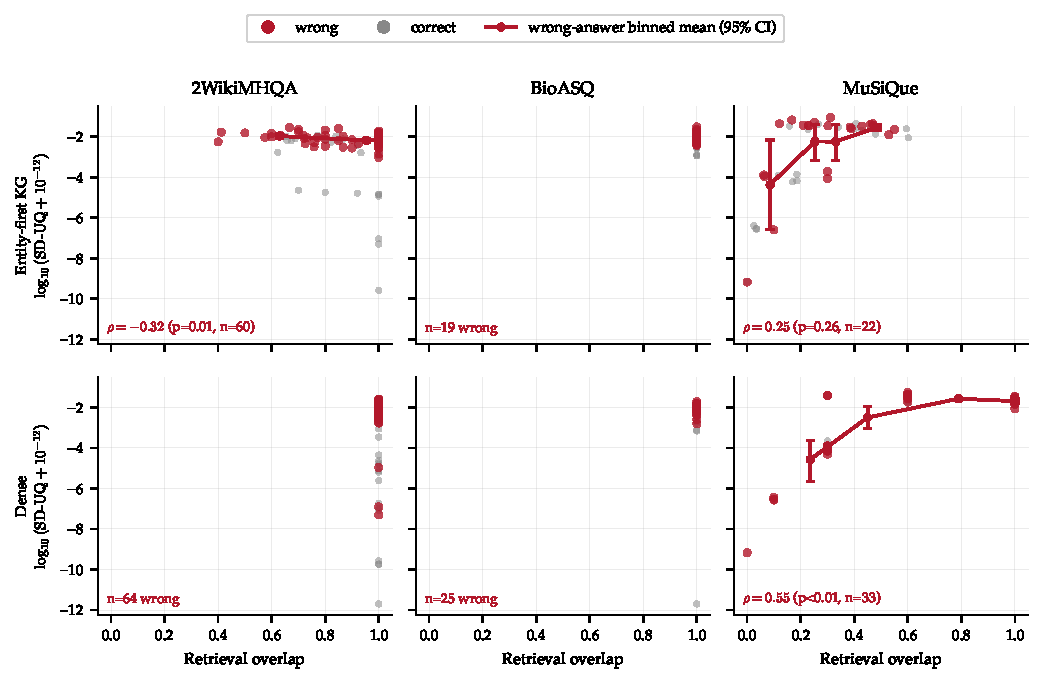
\includegraphics[width=0.92\linewidth]{figures/concentration_facets}
\caption{%
  \textbf{Full per-dataset, per-system view of the archived
  concentration--dispersion traces}, with per-dataset Spearman
  correlations among wrong answers and binned means with bootstrap $95\%$
  CIs.
  The KG-side coupling is carried by the bridge-style 2WikiMHQA trace;
  BioASQ overlap is saturated at $1.0$ (no within-dataset variation to
  correlate), and MuSiQue's small wrong set trends positive. These details keep
  the pooled $\rho=-0.27$ from being read as a between-dataset artefact or as a
  universal law.%
}
\label{fig:concentration_facets}
\end{figure*}


\begin{table*}[t]
\centering
\small
\caption{Selective risk at fixed coverage on the KG side: error rate among
the accepted questions when the most uncertain $20\%$ or $10\%$ are
abstained, using a single uncertainty signal as the gate.
``Base'' is the no-abstention error rate.
Under the adaptive policy, gating on SD-UQ alone is the strongest simple
policy; SEU gating is mediocre there because $25$--$74\%$ of adaptive rows
sit at the all-neutral $\mathrm{SEU}=0.5$ plateau, so the $80\%$ threshold
falls inside a tie mass (adaptive SEU cells are means over $200$ randomised
tie-breaking draws; the spread across draws is at most $0.006$).
Under the strict clinical ablation the ordering reverses: SD-UQ gating is no
better than accepting everything, while SEU gating removes roughly one in
five residual errors at $80\%$ coverage.
The 2WikiMultiHopQA strict run is the regime where no scalar gate helps,
consistent with the dataset-dependent survival reported in
Section~\ref{sec:results_grounding}.
\label{tab:operating_points}}
\setlength{\tabcolsep}{4pt}
\begin{tabular}{@{}lcccccc@{}}
\toprule
Run & $n$ & Base err. & SD@90\% & SD@80\% & SEU@80\% & Combined@80\% \\
\midrule
PubMedQA adaptive & 100 & 0.270 & 0.222 & 0.175 & 0.243 & 0.200 \\
RealMedQA adaptive & 223 & 0.054 & 0.030 & 0.022 & 0.054 & 0.034 \\
HotpotQA adaptive & 238 & 0.395 & 0.393 & 0.384 & 0.405 & 0.395 \\
HotpotQA FullWiki adaptive & 218 & 0.335 & 0.296 & 0.282 & 0.312 & 0.293 \\
2WikiMHQA adaptive & 244 & 0.311 & 0.282 & 0.256 & 0.261 & 0.267 \\
MuSiQue adaptive & 94 & 0.606 & 0.600 & 0.573 & 0.547 & 0.533 \\
\midrule
RealMedQA strict & 200 & 0.330 & 0.328 & 0.338 & 0.269 & 0.300 \\
2WikiMHQA strict & 245 & 0.592 & 0.600 & 0.633 & 0.668 & 0.617 \\
\bottomrule
\end{tabular}
\end{table*}

\begin{table}[t]
\centering
\small
\caption{Silent-failure sensitivity ladder: pooled fraction of wrong answers
classified as silent under progressively relaxed definitions of answer-state
dispersion.
With $N=5$ samples DSE is quantised, so $\mathrm{DSE} \leq 0.51$ admits at
most one dissenting sample (a 4-of-5 agreement gives
$\mathrm{DSE}=0.5004$).
The headline definition in Table~\ref{tab:silent_failures} is the most
conservative rung.
\label{tab:silent_sensitivity}}
\setlength{\tabcolsep}{4pt}
\begin{tabular}{@{}lccc@{}}
\toprule
Silent-error definition & Dense & Adaptive KG & Strict KG \\
\midrule
DSE $=0$ and SD-UQ at floor (headline) & 0.59 & 0.42 & 0.84 \\
DSE $=0$, any SD-UQ (unanimous)        & 0.67 & 0.52 & 0.88 \\
DSE $\leq 0.51$ ($\leq$1 dissenting sample) & 0.84 & 0.69 & 0.92 \\
\bottomrule
\end{tabular}
\end{table}

\begin{table}[t]
\centering
\small
\caption{Verbalised-confidence baseline (original P(True) protocol): the
generator backbone is asked once per saved answer for the probability that
the answer is correct, and $1-p$ is scored as uncertainty against the
paper's correctness labels.
No retrieval or generation is rerun.
AUROC treats incorrect answers as the positive class; SD-UQ columns repeat
the sampled-dispersion values for comparison.
The probe is competitive on the HotpotQA variants, weaker than SD-UQ on
RealMedQA, near chance on bridge-style 2WikiMultiHopQA under both policies,
and, unlike sampled dispersion, survives the strict clinical ablation.
\label{tab:verbalized_confidence}}
\setlength{\tabcolsep}{4.5pt}
\begin{tabular}{@{}lcc@{}}
\toprule
Run & Verbalised AUROC & SD-UQ AUROC \\
\midrule
PubMedQA adaptive & 0.55 & 0.70 \\
RealMedQA adaptive & 0.65 & 0.81 \\
HotpotQA adaptive & 0.72 & 0.64 \\
HotpotQA FullWiki adaptive & 0.77 & 0.67 \\
2WikiMHQA adaptive & 0.49 & 0.69 \\
MuSiQue adaptive & 0.65 & 0.63 \\
\midrule
RealMedQA strict & 0.89 & 0.23 \\
2WikiMHQA strict & 0.58 & 0.52 \\
\midrule
Pooled adaptive KG & 0.69 & -- \\
\bottomrule
\end{tabular}
\end{table}

\begin{table}[t]
\centering
\small
\caption{Mean marginal compute time per question for each diagnostic on the
KG side, averaged over the six headline runs (MacBook Pro M4; NLI on CPU).
Times are \emph{marginal}: they exclude the shared $N=5$ answer-sampling
calls that every answer-state estimator requires (the dominant
latency and token cost) and the cached NLI clustering shared by the
entropy-family scores.
GPS varies with graph depth (its maximum, $12.3$\,s, is the $h=4$ MuSiQue
configuration; the clinical graph costs $0.06$\,s).
\label{tab:compute_cost}}
\setlength{\tabcolsep}{5pt}
\begin{tabular}{@{}llr@{}}
\toprule
Diagnostic & Extra inputs & Mean time (s) \\
\midrule
DSE / P(True) proxy & cached NLI clusters & $<10^{-4}$ \\
SelfCheckGPT & $O(N^2)$ NLI calls & 1.68 \\
SRE-UQ & embeddings & 0.040 \\
VN-Entropy & embeddings & 0.007 \\
SD-UQ & embeddings & 0.012 \\
SEU & $K$ NLI calls & 1.65 \\
GPS & graph queries & 2.43 (0.06--12.3) \\
\bottomrule
\end{tabular}
\end{table}



\begin{table*}[t]
\centering
\small
\caption{HotpotQA FullWiki $n=250$ shared-corpus stress run.
Vanilla uses dense retrieval; KG-RAG uses the reported entity-first policy
with fallback.
Clean accuracy excludes provider-side generation failures.
GPS AUROC is reported only for KG-RAG because GPS is a graph-state diagnostic;
the GPS null rate is the fraction of answered KG rows for which the metric is
unavailable or falls back.
\label{tab:hotpot_fullwiki_stress}}
\setlength{\tabcolsep}{4pt}
\begin{tabular}{@{}lccccccccc@{}}
\toprule
Policy & Ans. & Clean acc. & Raw acc. & DSE & SRE-UQ & VN-Ent. & SD-UQ & SEU & GPS / null \\
\midrule
Dense vanilla & 208 & 0.721 & 0.600 & 0.650 & 0.630 & 0.666 & 0.665 & 0.563 & -- \\
Entity-first KG & 218 & 0.665 & 0.580 & 0.666 & 0.688 & 0.701 & 0.672 & 0.565 & 0.543 / 0.151 \\
\bottomrule
\end{tabular}
\end{table*}

\begin{table*}[t]
\centering
\small
\caption{Post-hoc RealMedQA GPS replay on the full $n=230$ answer logs.
No generation, retrieval, or LLM call was rerun; only GPS
was recomputed against the persistent dataset KG.
``Old'' is the original surface-matched, binary-reachability GPS;
``new'' is the final soft-linked, depth-matched estimator of
Section~\ref{sec:struct_metrics}.
The linking threshold and decay ($\tau=0.60$, $\gamma=0.4$) were selected on
this dataset and applied frozen everywhere else, so this table shows
calibrated in-domain behaviour; the open-domain tables provide the held-out
estimate.
\label{tab:realmedqa_replay}}
\begin{tabular}{@{}lccc@{}}
\toprule
Setting & Answered & GPS usable (old$\rightarrow$new) & GPS AUROC (old$\rightarrow$new) \\
\midrule
Dense + vanilla & 219 & 100 $\rightarrow$ 192 & 0.72 $\rightarrow$ 0.89 \\
Entity-first + KG & 223 & 97 $\rightarrow$ 195 & 0.47 $\rightarrow$ 0.76 \\
\bottomrule
\end{tabular}
\end{table*}

\begin{table*}[t]
\centering
\small
\caption{RealMedQA no-rebuild strict graph-only stress test on the full
$n=230$ question set.
The adaptive row is the reported KG policy from the full RealMedQA run.
The strict row reuses the same RealMedQA graph, disables dense fallback,
vector augmentation, and decomposition, and therefore tests whether a more
concentrated entity-first retrieval regime compresses answer-state
uncertainty.
All metric columns report AUROC.
\label{tab:realmedqa_strict_entity}}
\setlength{\tabcolsep}{3.5pt}
\begin{tabular}{@{}lcccccccc@{}}
\toprule
KG policy & Ans. & Acc. & Overlap & DSE & VN & SD-UQ & SEU & GPS \\
\midrule
Adaptive + fallback & 223 & 0.946 & 0.558 & 0.699 & 0.815 & 0.808 & 0.501 & 0.76$^\dagger$ \\
Strict graph-only & 200 & 0.670 & 0.661 & 0.463 & 0.248 & 0.233 & 0.721 & 0.746$^\dagger$ \\
\bottomrule
\end{tabular}

\vspace{0.4em}
\raggedright\footnotesize
$^\dagger$ GPS values come from the post-hoc replay
(Table~\ref{tab:realmedqa_replay}): adaptive $195/223$ usable rows, strict
$142/200$.
RealMedQA is the calibration domain for the GPS hyperparameters, so these
cells show calibrated in-domain behaviour; Table~\ref{tab:gps_reliability_bins}
gives the corresponding binned error-rate view.
\end{table*}

\paragraph{Depth-matched GPS scoring.}
GPS uses a depth-matched decay, $\gamma^{|L_e - \hat{L}|}$, where $\hat{L}$ is
the expected reasoning depth: the question's logged hop count where available
(2WikiMultiHopQA, MuSiQue), the dataset's nominal depth by construction
(HotpotQA variants, $\hat{L}=2$), and $\hat{L}=1$ otherwise.
Because $\hat{L}=1$ on RealMedQA, the calibration domain is untouched and the
frozen $(\tau, \gamma)$ carry over; all other rows are single-shot
evaluations of the same declared definition.
This is the GPS definition used in all main tables.

\begin{table*}[t]
\centering
\scriptsize
\caption{Percentile-bootstrap 95\% intervals for the headline answer-state and
evidence-state AUROCs.
These are the main answer-side metrics used in the narrative: SRE-UQ and
SD-UQ as the practical answer-state baselines, and SEU as the evidence-state signal.
The table is intended to calibrate scale, not to claim significance testing
for every pairwise gap.
\label{tab:headline_ci_output}}
\begin{tabular}{@{}lcccccc@{}}
\toprule
Dataset & SRE-UQ Van. & SRE-UQ KG & SD-UQ Van. & SD-UQ KG & SEU Van. & SEU KG \\
\midrule
PubMedQA & 0.56 [0.49, 0.64] & 0.64 [0.55, 0.73] & 0.60 [0.46, 0.74] & 0.70 [0.57, 0.81] & 0.55 [0.44, 0.67] & 0.59 [0.47, 0.71] \\
RealMedQA & 0.43 [0.24, 0.62] & 0.66 [0.51, 0.80] & 0.63 [0.39, 0.86] & 0.81 [0.64, 0.94] & 0.63 [0.47, 0.79] & 0.50 [0.35, 0.63] \\
HotpotQA & 0.61 [0.54, 0.68] & 0.63 [0.57, 0.70] & 0.64 [0.56, 0.72] & 0.64 [0.56, 0.70] & 0.46 [0.39, 0.54] & 0.48 [0.40, 0.55] \\
HotpotQA FullWiki & 0.63 [0.55, 0.71] & 0.69 [0.60, 0.76] & 0.66 [0.58, 0.75] & 0.67 [0.60, 0.75] & 0.56 [0.47, 0.65] & 0.56 [0.49, 0.64] \\
2WikiMHQA & 0.59 [0.52, 0.67] & 0.65 [0.58, 0.72] & 0.61 [0.52, 0.69] & 0.69 [0.61, 0.75] & 0.62 [0.53, 0.70] & 0.64 [0.57, 0.72] \\
MuSiQue & 0.64 [0.53, 0.75] & 0.66 [0.56, 0.77] & 0.67 [0.55, 0.78] & 0.63 [0.52, 0.75] & 0.63 [0.52, 0.75] & 0.63 [0.51, 0.74] \\
\bottomrule
\end{tabular}
\end{table*}

% =============================================================================
\section{Extended Results and Robustness Analyses}
\label{sec:appendix_extended}

This section collects secondary analyses referenced from
Section~\ref{sec:results}: silent-error threshold sensitivity, the archived
concentration--dispersion traces, the within-adaptive stability check, the
verbalised-confidence baseline, family disagreement, and the simple composite
audit score.

\subsection{Silent-Error Threshold Sensitivity}
\label{sec:appendix_silent_sensitivity}

The exact-floor silent-error definition used in
Table~\ref{tab:silent_failures} is conservative: requiring only unanimous
sampled answers (DSE $=0$, any SD-UQ) raises the pooled rates to
$52\%$/$67\%$/$88\%$ (adaptive KG / dense / strict), and admitting one
dissenting sample out of five raises them to $69\%$/$84\%$/$92\%$
(Table~\ref{tab:silent_sensitivity}), so the headline definition understates
rather than inflates the blind spot.
Unanimity at $N=5$ is already informative: if the modal answer held only
$0.7$ probability, five identical samples would occur with probability
$0.7^5 \approx 0.17$.
Two $20$-sample probes confirm the mass is not a budget artefact in the
analysed snapshots.
On the strict clinical subset, all $24$ empty-route wrong answers stay
perfectly unanimous at $N{=}20$ ($\mathrm{DSE}=0$ for every row; SD-UQ AUROC
$0.17$, unchanged from $N{=}5$).
On \emph{dense} 2WikiMultiHopQA (a pure non-graph retriever), $68\%$ of wrong
answers remain strictly silent and $86\%$ stay within one dissenting sample of
twenty, against $79\%$ strictly silent at $N{=}5$ on the headline run (the
$N{=}20$ probe uses an $n{=}100$ subset and the $N{=}5$ headline an $n{=}250$
subset, so the level at $N{=}20$ is the robust statistic rather than the
precise $79\!\to\!68\%$ delta).
Quadrupling the budget therefore barely moves the silent rate, including on
a dense system with no graph state.
These probes are deliberately narrow: they support persistence of the headline
failure mode, not a full sampling-budget sweep across every adaptive and strict
KG setting.

\subsection{Interventional Dose-Response}
\label{sec:appendix_doseresponse}

The strict-clinical collapse summarised in
Section~\ref{sec:results_collapse} is not a chunk-level stochasticity
artefact.
An interventional dose-response holds the graph, policy, prompts, and
questions fixed ($n=100$, seed 42) and varies only final-stage retrieval
determinism, sampling the final $k{=}10$ chunks from a $4k$ shortlist at
retrieval temperature $\{0, 0.5, 1.0\}$.
The manipulation works: mean within-question chunk overlap falls from
$0.67$ to $0.29$, a $57\%$ reduction. Yet the collapse does not move: SD-UQ
AUROC is $0.18/0.18/0.16$ across doses and the silent-error count is identical
($24$ of $29$--$30$ wrong, with the same $24/24$ empty-retrieval rows in each
arm).
Chunk-level stochasticity therefore does not dislodge the lock-in; the route
decomposition in Section~\ref{sec:results_collapse} locates the silent mass in
the empty-retrieval state instead.

\subsection{Archived Concentration--Dispersion Traces}
\label{sec:appendix_concentration}

Direct per-question evidence comes from three archived traces that retained
per-question retrieval overlap
(2WikiMultiHopQA $n=100$, BioASQ $n=57$, MuSiQue $n=66$;
Figure~\ref{fig:concentration_facets}).
Among \emph{wrong} KG answers the pooled coupling is negative
(Spearman $\rho = -0.27$, $p = 0.006$, $n = 101$): the more concentrated the
retrieval state, the lower the wrong-answer dispersion.
The coupling is carried by 2WikiMultiHopQA ($\rho = -0.32$, $p = 0.01$,
$n = 60$), the bridge-style dataset where lock-in is sharpest.
BioASQ's archived overlap is saturated at $1.0$, and MuSiQue's small
wrong-answer set trends the other way ($\rho = +0.25$, $n = 22$, n.s.).
On the dense side the coupling is absent where overlap is near-deterministic
and positive on MuSiQue ($\rho = +0.55$), nothing like the KG-side bridge
pattern.
These archived traces support, but do not identify, the mechanism.

\subsection{Within-Adaptive Stability Check}
\label{sec:appendix_within_stability}

An archived 2WikiMultiHopQA $n=100$ trace, unlike the newer $n=250$ run,
retained per-question chunk-overlap fields;
Table~\ref{tab:within_adaptive_stability} uses it for a small
within-adaptive sanity check.
The high-overlap band is not a monotone proof of collapse, but a useful
warning case: accuracy falls to $0.294$, DSE AUROC is near chance at $0.467$,
and VN-Entropy AUROC falls to $0.583$.
SD-UQ still carries moderate signal ($0.633$), so the result should be read
carefully.
High-stability strata thus exist inside an adaptive policy, but the logger
must persist per-question chunk, entity, and path overlap before this can be
made a headline claim.

\begin{table*}[t]
\centering
\small
\caption{%
  Within-adaptive retrieval-stability sanity check from an archived
  2WikiMultiHopQA $n=100$ trace that retained per-question chunk-overlap
  fields.  The newer $n=250$ run is the headline result; this table is a
  mechanism check.
  Bands are population tertiles of per-question chunk overlap; because a
  large fraction of questions sit at exactly $1.0$ overlap, ties spill
  across the tertile boundary.
  AUROC treats incorrect answers as the positive class.%
}
\label{tab:within_adaptive_stability}
\setlength{\tabcolsep}{3.5pt}
\begin{tabular}{@{}lrrrrrrr@{}}
\toprule
Overlap band & $n$ & Range & Acc. & DSE AUC & SD AUC & VN AUC & DSE mean \\
\midrule
Low & 33 & 0.400--0.840 & 0.364 & 0.415 & 0.714 & 0.750 & 0.277 \\
Medium & 33 & 0.850--1.000 & 0.545 & 0.667 & 0.800 & 0.752 & 0.103 \\
High & 34 & 1.000--1.000 & 0.294 & 0.467 & 0.633 & 0.583 & 0.157 \\
\bottomrule
\end{tabular}
\end{table*}


\subsection{Dedicated Per-Sample Graph-State Diversity Run}
\label{sec:appendix_diversity}

Table~\ref{tab:diversity_run} in the main text comes from a run built solely to
close the logging gap noted above: the archived traces persisted chunk overlap
alone, so the coupling could only ever be a warning case.
The diversity run was executed on HotpotQA-FullWiki ($n=221$ answered questions
with complete per-sample traces, $74$ of them wrong), reusing the existing
FullWiki knowledge graph with no rebuild, and recording for every question the
mean pairwise Jaccard overlap across the $N=5$ samples for four retrieval-state
families, namely the matched seed entities, the traversed paths, the assembled
subgraph, and the retrieved chunks, together with the per-question SD-UQ used
for the coupling test.
The two halves it confirms, a near-stable retrieval state across samples
(the premise Equation~\eqref{eq:collapsed} assumes) and a negative
overlap--dispersion coupling among wrong answers, are reported in the main
text.
The seed-entity coupling there is null only because seed overlap saturates near
$1.0$, leaving almost no variance to correlate against.
The sign and magnitude of the path, subgraph, and chunk couplings match the
archived 2WikiMultiHopQA trace of Section~\ref{sec:appendix_concentration} on
independent data and across the full set of overlap families, so the coupling no
longer rests on chunk overlap from a single archived run.

\subsection{Verbalised-Confidence Baseline}
\label{sec:appendix_verbalized}

The verbalised-confidence baseline summarised in
Section~\ref{sec:results_output} uses the original P(True) protocol, which
asks the model for a probability rather than counting cluster agreement and is
therefore not blind to silent errors by construction.
Querying the same backbone once per saved answer
(Table~\ref{tab:verbalized_confidence}) yields pooled adaptive-KG
AUROC $0.69$: competitive on the HotpotQA variants ($0.72$/$0.77$, above
SD-UQ there), weaker than SD-UQ on RealMedQA ($0.65$ vs.\ $0.81$), and near
chance precisely where bridge-style lock-in lives (2WikiMultiHopQA: $0.49$
adaptive, $0.58$ strict).
On the strict clinical ablation it reaches $0.89$ while sampled dispersion
collapses to $0.233$, so part of the clinical silent-error mass is
recoverable from the generator's own self-estimate without any retrieval-side
signal.
If a one-call self-estimate can flag clinical silent errors, why decompose at
all?
First, it fails on bridge-style lock-in
($0.49$--$0.58$), the regime the decomposition targets: where the wrong
answer is parametrically plausible, \emph{no} output-side signal tested
here, sampled or verbalised, ranks the errors.
Second, a verbalised probability is an uncalibrated self-report with known
self-preference pathologies, whereas SEU and GPS are grounded in visible
evidence and graph state.
Third, the self-estimate returns a number without a reason: when it
disagrees with the answer there is no provenance to audit, which is precisely
the evidence a clinical review workflow would need.

\subsection{Family Disagreement and the Simple Composite Audit Score}
\label{sec:appendix_composite}

\begin{figure*}[t]
\centering
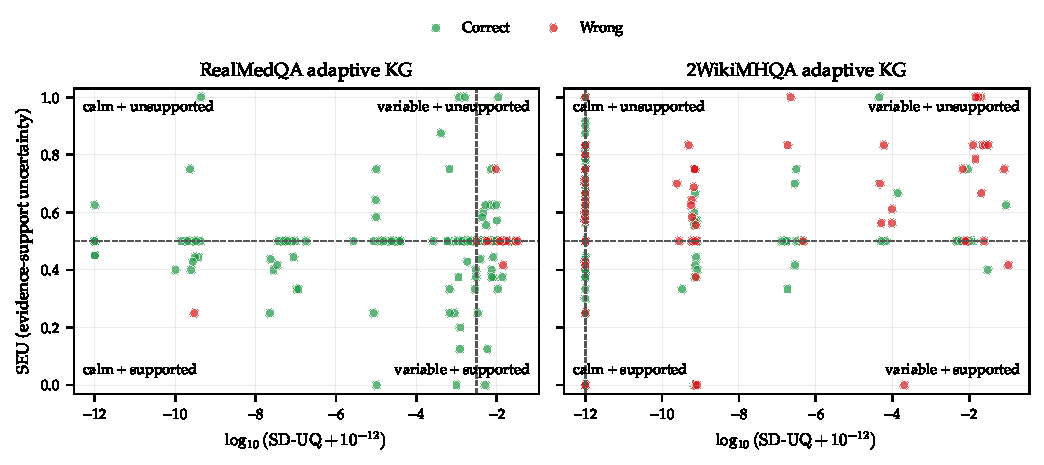
\includegraphics[width=\linewidth]{figures/family_disagreement_scatter}
\caption{%
  \textbf{Family disagreement in the pooled adaptive KG runs.}
  Grey hexagons show the density of all answered questions with a
  non-neutral SEU verdict; red points overlay the wrong answers.
  The $x$-axis is answer-state residual dispersion (SD-UQ, log scale) and
  the $y$-axis is evidence-state uncertainty (SEU).
  The all-neutral $\mathrm{SEU}=0.5$ rows, where the NLI head said nothing
  ($n=464$, $24\%$ wrong), are excluded.
  Dashed lines mark the pooled SD-UQ median and $\mathrm{SEU}=0.5$; the two
  low-answer-uncertainty quadrants carry the decision-relevant contrast:
  low answer uncertainty with contradicted evidence is $31\%$ wrong against
  $20\%$ for low answer uncertainty with support, so answer-surface agreement
  is not a proxy for evidence support.%
}
\label{fig:family_disagreement}
\end{figure*}

Beyond the conjunctive audit rule of Section~\ref{sec:results_composite},
Table~\ref{tab:composite_audit_score} gives a deliberately simple audit score:
the mean of within-dataset percentile ranks for SD-UQ, SEU, and final GPS-risk,
with GPS abstention treated as high risk.
It is uneven and not claimed to dominate the best answer-state metric.
The PubMedQA row shows where the combination earns its keep: GPS abstains on
every yes/no row (flat $0.5$), yet Combined reaches $0.813$ against SD-UQ's
$0.699$, because SEU contributes complementary support-level ranking exactly
where answer dispersion is coarse, not because the abstaining family adds
signal.
Its purpose is to show how the reported families can feed a decision layer;
a deployable policy would still need held-out calibration.

\begin{table*}[t]
\centering
\small
\caption{Adaptive-KG composite audit score.  The combined score is the mean of within-dataset percentile ranks for SD-UQ, SEU, and final GPS-risk, with GPS abstention treated as high risk.  AUROC treats incorrect answers as the positive class.  ``Base err.''\ is the no-abstention error rate; lower AUREC is better within a dataset.  ``Best single'' is the largest per-family AUROC in the row.}
\label{tab:composite_audit_score}
\setlength{\tabcolsep}{4pt}
\begin{tabular}{@{}lrrrrrrrr@{}}
\toprule
Dataset & $n$ & Base err. & SD-UQ AUC & SEU AUC & GPS-risk AUC & Best single & Combined AUC & Combined AUREC \\
\midrule
PubMedQA & 100 & 0.270 & 0.699 & 0.594 & 0.500 & 0.699 & \textbf{0.813} & 0.096 \\
RealMedQA & 223 & 0.054 & 0.808 & 0.501 & 0.703 & \textbf{0.808} & 0.729 & 0.022 \\
HotpotQA & 238 & 0.395 & 0.635 & 0.477 & 0.551 & \textbf{0.635} & 0.573 & 0.326 \\
HotpotQA FullWiki & 218 & 0.335 & 0.672 & 0.565 & 0.549 & \textbf{0.672} & 0.661 & 0.228 \\
2WikiMHQA & 244 & 0.311 & 0.685 & 0.643 & 0.414 & \textbf{0.685} & 0.619 & 0.225 \\
MuSiQue & 94 & 0.606 & 0.631 & 0.626 & 0.640 & 0.640 & \textbf{0.745} & 0.426 \\
\bottomrule
\end{tabular}
\end{table*}


\subsection{GPS Hyperparameter Sensitivity}
\label{sec:appendix_gps_sensitivity}

To test whether the headline GPS AUROCs depend on the two calibrated
hyperparameters, the soft-link threshold $\tau$ and the distance decay $\gamma$
are swept over $\tau \in \{0.50, 0.55, 0.60, 0.65, 0.70\}$ and
$\gamma \in \{0.2, 0.4, 0.6, 0.8, 1.0\}$ ($25$ cells), recomputed by offline
replay from the saved GPS replay stores. No generation, retrieval, linking, or KG
build is rerun.
Table~\ref{tab:gps_sensitivity} reports the calibrated cell (which reproduces
the headline numbers), the AUROC range across the grid, its standard deviation,
and the usable-row range.
The held-out open-domain AUROCs are robust to the hyperparameters (standard
deviation $\leq 0.018$ on HotpotQA, HotpotQA FullWiki, 2WikiMultiHopQA, and
MuSiQue), so the open-domain weakness, including the below-chance
2WikiMultiHopQA score, is a genuine retrieval limitation rather than a tuning
artefact.
The clinical calibration domain is the most sensitive ($0.038$ adaptive,
$0.091$ strict), as expected for the dataset the hyperparameters were tuned on.

\begin{table}[t]
\centering
\small
\caption{GPS AUROC sensitivity to $(\tau, \gamma)$ by offline replay.
``Calib.'' is the paper's frozen $\tau{=}0.60$, $\gamma{=}0.40$ cell; range,
SD, and usable counts are over the $5\times5$ grid.
\label{tab:gps_sensitivity}}
\setlength{\tabcolsep}{4pt}
\begin{tabular}{@{}lcccc@{}}
\toprule
Run & Calib. & Grid range & SD & Usable \\
\midrule
RealMedQA adaptive & 0.76 & 0.60--0.76 & 0.038 & 191--197 \\
RealMedQA strict   & 0.75 & 0.53--0.90 & 0.091 & 139--171 \\
HotpotQA           & 0.51 & 0.50--0.55 & 0.014 & 154--169 \\
HotpotQA FullWiki  & 0.54 & 0.53--0.56 & 0.008 & 182--187 \\
2WikiMHQA adaptive & 0.38 & 0.35--0.40 & 0.012 & 177--188 \\
2WikiMHQA strict   & 0.48 & 0.40--0.53 & 0.035 & 94--104 \\
MuSiQue            & 0.68 & 0.64--0.70 & 0.018 & 80--85 \\
\bottomrule
\end{tabular}
\end{table}

\subsection{Audit of the Fully Unflagged Residue}
\label{sec:appendix_residue}

Of the $141$ pooled adaptive-KG silent errors, $7$ ($5\%$) are unflagged by
every non-answer family (Section~\ref{sec:results_collapse}): not on an empty route,
$\mathrm{SEU}\leq 0.5$, and GPS defined and $\leq 0.5$.
A manual audit of all seven from the saved logs (question, gold answer,
generated answer) characterises them as two benchmark-ambiguous or
contested-label questions (e.g.\ the founding year of an institution with a
disputed predecessor date; a subjective ``more known for'' comparison), two
wrong-answer-slot errors where the model returns a question anchor rather than
the asked attribute (e.g.\ naming a song's performer instead of their cause of
death), and three parametric conflations or specificity mismatches (e.g.\
returning a film character's love interest instead of the lead actress's real
spouse).
SEU sits at its neutral $0.5$ default on four of the seven and below it on the
other three, so it abstains or mildly supports rather than flagging by
construction none exceed $0.5$.
Crucially, retrieved chunk texts are not archived, so none can be confirmed as
deep presence lock-in whose evidence \emph{entails} the wrong answer; the
residue is therefore better read as a mixture of label ambiguity, answer-slot
errors, and parametric overconfidence than as a wall of undetectable lock-in.

\subsection{Relocated Diagnostic Tables}
\label{sec:appendix_relocated}

Two diagnostic tables referenced from the main text are collected here to keep
the results flow tight.
Table~\ref{tab:failure_modes} summarises, per family, the regime each
diagnostic detects and where it goes silent.
Table~\ref{tab:twowiki_hopwise_diagnostics} gives the full hop-stratified
2WikiMultiHopQA comparison across the three retrieval policies; its decisive
row, the strict graph-only 4-hop slice with zero clean accuracy and collapsed
SD-UQ and VN-Entropy, is discussed in Section~\ref{sec:results_collapse}.
The table uses clean answered rows rather than raw hop-bucket sizes, so $n$
differs across policies when provider failures or skipped systems remove
rows, the same convention used for clean accuracy.

% Figure: Diagnostic behaviour across retrieval regimes.
% Full-width matrix. Include with: % Figure: Diagnostic behaviour across retrieval regimes.
% Full-width matrix. Include with: \input{figures/metric_failure_modes}

\begin{table*}[t]
\centering
\small
\setlength{\tabcolsep}{4pt}
\renewcommand{\arraystretch}{1.25}
\begin{tabular}{@{}p{0.15\linewidth}p{0.27\linewidth}p{0.13\linewidth}p{0.11\linewidth}p{0.11\linewidth}p{0.15\linewidth}@{}}
\toprule
\textbf{Retrieval regime}
&
\textbf{State of the context}
&
\textbf{Answer-state}
&
\textbf{SEU}
&
\textbf{GPS}
&
\textbf{Reading} \\
\midrule
Anchor failure
&
Entity linking fails; system falls back to text retrieval.
&
$\sim$~variation may persist
&
$\sim$~fallback passages
&
$\oslash$~abstains
&
Absence of a graph object is itself diagnostic. \\
\addlinespace[0.25em]
Stabilised retrieval
&
Same or near-same graph neighbourhood across samples.
&
$\downarrow$~compressed
&
\checkmark~support / contradiction
&
\checkmark~consistency
&
Agreement should be read against evidence and graph. \\
\addlinespace[0.25em]
Wrong coherent anchor
&
Anchoring succeeds on the wrong neighbourhood; paths locally coherent.
&
$\downarrow$~same wrong answer repeats
&
$\sim$~can warn
&
\texttimes~supports wrong state
&
Hardest lock-in case; trace inspection needed. \\
\addlinespace[0.25em]
KG incompleteness
&
Plausible anchor, but bridges or relations missing from the graph.
&
$\sim$~fallback restores variation
&
\checkmark~if text remains
&
$\oslash$/$\sim$~reduced
&
Coverage or construction error, not decoder uncertainty. \\
\bottomrule
\end{tabular}

\caption{%
  \textbf{Expected diagnostic behaviour across KG-RAG retrieval regimes.}
  Symbols: \checkmark~informative; $\sim$~partially informative;
  $\downarrow$~compressed and potentially silent; $\oslash$~abstains;
  \texttimes~locally consistent with a wrong state.
  Each cell states what a family can observe, not a ranking;
  Table~\ref{tab:decomposition} defines the families and
  Table~\ref{tab:failure_taxonomy} gives the resulting $2{\times}2$
  taxonomy.%
}
\label{tab:failure_modes}
\end{table*}


\begin{table*}[t]
\centering
\small
\setlength{\tabcolsep}{4pt}
\renewcommand{\arraystretch}{1.25}
\begin{tabular}{@{}p{0.15\linewidth}p{0.27\linewidth}p{0.13\linewidth}p{0.11\linewidth}p{0.11\linewidth}p{0.15\linewidth}@{}}
\toprule
\textbf{Retrieval regime}
&
\textbf{State of the context}
&
\textbf{Answer-state}
&
\textbf{SEU}
&
\textbf{GPS}
&
\textbf{Reading} \\
\midrule
Anchor failure
&
Entity linking fails; system falls back to text retrieval.
&
$\sim$~variation may persist
&
$\sim$~fallback passages
&
$\oslash$~abstains
&
Absence of a graph object is itself diagnostic. \\
\addlinespace[0.25em]
Stabilised retrieval
&
Same or near-same graph neighbourhood across samples.
&
$\downarrow$~compressed
&
\checkmark~support / contradiction
&
\checkmark~consistency
&
Agreement should be read against evidence and graph. \\
\addlinespace[0.25em]
Wrong coherent anchor
&
Anchoring succeeds on the wrong neighbourhood; paths locally coherent.
&
$\downarrow$~same wrong answer repeats
&
$\sim$~can warn
&
\texttimes~supports wrong state
&
Hardest lock-in case; trace inspection needed. \\
\addlinespace[0.25em]
KG incompleteness
&
Plausible anchor, but bridges or relations missing from the graph.
&
$\sim$~fallback restores variation
&
\checkmark~if text remains
&
$\oslash$/$\sim$~reduced
&
Coverage or construction error, not decoder uncertainty. \\
\bottomrule
\end{tabular}

\caption{%
  \textbf{Expected diagnostic behaviour across KG-RAG retrieval regimes.}
  Symbols: \checkmark~informative; $\sim$~partially informative;
  $\downarrow$~compressed and potentially silent; $\oslash$~abstains;
  \texttimes~locally consistent with a wrong state.
  Each cell states what a family can observe, not a ranking;
  Table~\ref{tab:decomposition} defines the families and
  Table~\ref{tab:failure_taxonomy} gives the resulting $2{\times}2$
  taxonomy.%
}
\label{tab:failure_modes}
\end{table*}


\begin{table*}[t]
\centering
\small
\caption{%
  Hop-wise 2WikiMultiHopQA diagnostics on the same fixed $n=250$ subset.
  The table uses clean answered rows; $n_{\mathrm{w}}$ is the AUROC positive
  class.
  AUROC is omitted when a hop slice has only one correctness class.
  The $\geq$5-hop bucket contains four questions and is kept only in the
  released JSON artefact.%
}
\label{tab:twowiki_hopwise_diagnostics}
\setlength{\tabcolsep}{3.4pt}
\begin{tabular}{@{}llrrrrrrrrrr@{}}
\toprule
Policy & Hop & $n$ & $n_{\mathrm{w}}$ & Acc. & SD mean & VN mean & SEU mean &
SD AUC & VN AUC & SEU AUC & GPS AUC \\
\midrule
Dense vanilla & 2-hop & 150 & 42 & 0.720 & 0.000 & 0.092 & 0.612 & 0.615 & 0.639 & 0.615 & 0.491 \\
Dense vanilla & 4-hop & 58 & 16 & 0.724 & 0.000 & 0.198 & 0.458 & 0.628 & 0.571 & 0.656 & 0.410 \\
Adaptive KG & 2-hop & 182 & 57 & 0.687 & 0.003 & 0.191 & 0.544 & 0.702 & 0.668 & 0.611 & 0.335 \\
Adaptive KG & 4-hop & 58 & 16 & 0.724 & 0.002 & 0.248 & 0.466 & 0.600 & 0.638 & 0.646 & 0.452 \\
Strict KG & 2-hop & 183 & 83 & 0.546 & 0.003 & 0.127 & 0.569 & 0.560 & 0.680 & 0.378 & 0.353 \\
Strict KG & 4-hop & 58 & 58 & 0.000 & 0.000 & 0.000 & 0.500 & -- & -- & -- & -- \\
\bottomrule
\end{tabular}
\end{table*}


% =============================================================================
\section{Additional Qualitative Cases}
\label{sec:appendix_cases}

\begin{table*}[t]
\centering
\small
\setlength{\tabcolsep}{4pt}
\renewcommand{\arraystretch}{1.2}
\caption{%
  \textbf{Consolidated case gallery from the reported runs.}
  \texttimes{} rows are verified lock-in failures: the KG answer is wrong yet
  repeated across all samples ($\mathrm{DSE}=0$, SD-UQ at or near the floor);
  the diagnostic columns show which family, if any, still fires.
  \checkmark{} rows are KG successes on bridge questions, where the same
  retrieval stability is helpful because the path reaches the right entity
  and relation, plus one correct answer despite GPS abstention.
  The Baltic Cup row is the hardest failure: the retrieved evidence
  \emph{entails} the wrong answer, so every scalar family reports low risk and
  only the provenance trace remains auditable.
  GPS $=0.5$ denotes abstention.
  The cases are selected for illustration, not sampled; prevalence claims
  rest on Tables~\ref{tab:silent_failures} and
  \ref{tab:failure_taxonomy}, not on this gallery.%
}
\label{tab:lockin_gallery}
\begin{tabular}{@{}c>{\raggedright\arraybackslash}p{0.26\textwidth}
                  l
                  >{\raggedright\arraybackslash}p{0.22\textwidth}
                  l c c@{}}
\toprule
\textbf{KG} & \textbf{Question (dataset)} & \textbf{Gold} & \textbf{Anchor / path}
& \textbf{KG answer} & \textbf{SEU} & \textbf{GPS} \\
\midrule
\texttimes & Osireion is behind the temple of which pharaoh? (HotpotQA)
 & Seti I
 & \emph{Ramesses II} neighbourhood of the Abydos temple
 & Ramesses II & $1.00$ & $0.44$ \\
\texttimes & Who is the paternal grandfather of Uskhal Khan? (2Wiki)
 & Khutughtu Khan
 & \emph{Toghon Tem\"ur} (father, one hop; bridge skipped)
 & Toghon Tem\"ur & $0.60$ & $0.00$ \\
\texttimes & Who created Mickey Mouse's spouse? (MuSiQue)
 & Walt Disney
 & \emph{Ub Iwerks} via Mickey Mouse $\to$ creator
 & Ub Iwerks & $0.75$ & $0.00$ \\
\texttimes & Who is Ieuan ab Owain Glynd\^wr's paternal grandfather? (2Wiki)
 & Gruffudd Fychan II
 & \emph{Owain Glynd\^wr} (father, one hop; bridge skipped)
 & Owain Glynd\^wr & $0.43$ & $0.24$ \\
\texttimes & Which country skipped the 1991 Baltic Cup? (HotpotQA)
 & Belarus
 & \emph{Estonia} via Baltic Cup participants
 & Estonia & $0.00$ & $0.00$ \\
\texttimes & Are TEC-1 and Dubna 48K based on the same processor? (HotpotQA)
 & yes
 & weak graph state; no usable anchor, GPS abstains
 & no & $0.75$ & $0.50$ \\
\texttimes & 2010 population of the city popular with tourists? (MuSiQue)
 & 8.005 million
 & wrong city; only linkable answer string four hops away
 & 2{,}217 & $0.67$ & $0.94$ \\
\midrule
\checkmark & Who is the spouse of the director of \emph{Fire-Eater}? (2Wiki)
 & Pirkko Saisio
 & film $\to$ director $\to$ spouse bridge preserved
 & Pirkko Saisio & $0.60$ & $0.44$ \\
\checkmark & Who is the father of the director of \emph{The Cup} (1999)? (2Wiki)
 & Thinley Norbu
 & film $\to$ director $\to$ father bridge preserved
 & Thinley Norbu & $0.69$ & $0.35$ \\
\checkmark & Birthplace of the director of \emph{Dollar} (1938)? (2Wiki)
 & Helsingfors
 & film $\to$ director $\to$ birthplace bridge preserved
 & Helsingfors & $0.50$ & $0.60$ \\
\checkmark & Dow Jones fall at the highest US unemployment rate? (MuSiQue)
 & 54.7\%
 & chain resolved correctly; GPS still abstains
 & 54.7\% & $0.72$ & $0.50$ \\
\bottomrule
\end{tabular}
\end{table*}


Table~\ref{tab:lockin_gallery} is the canonical case gallery.
The failure rows follow the form wrong anchor $\to$ stable retrieved context
$\to$ stable wrong answer $\to$ silent answer surface, showing per case which
diagnostic family still responds; the success rows show the same retrieval
stability working as intended on 2WikiMHQA bridge questions, where the graph
preserves the intermediate entity that vanilla retrieval loses, plus one
MuSiQue chain resolved correctly despite GPS abstention.
The main text uses one path-faithfulness example
(the Osireion lock-in of Figure~\ref{fig:lockin_trace}) to keep the exposition
focused on the lock-in mechanism; the gallery provides trace evidence, not
additional leaderboard claims.
Table~\ref{tab:path_faithfulness_case} gives the full per-family audit readout
for that Osireion case (question, retrieved graph state, and the
DSE/SD-UQ/GPS/SEU verdicts), expanding the summary in
Section~\ref{sec:results_cases}.

\begin{table*}[t]
\centering
\small
\setlength{\tabcolsep}{5pt}
\renewcommand{\arraystretch}{1.2}
\caption{%
  \textbf{Path-faithfulness failure under retrieval lock-in (HotpotQA).}
  A wrong-but-graph-coherent case from the fixed-$n=250$ run.
  The retriever anchors to a strongly associated but incorrect
  Nineteenth-Dynasty pharaoh, and every sampled answer repeats it.
  Answer-state metrics are silent and GPS reports support; only SEU fires.%
}
\label{tab:path_faithfulness_case}
\begin{tabular}{@{}>{\raggedright\arraybackslash}p{0.30\textwidth}
                  >{\raggedright\arraybackslash}p{0.30\textwidth}
                  >{\raggedright\arraybackslash}p{0.33\textwidth}@{}}
\toprule
\textbf{Question and gold answer} &
\textbf{Retrieved graph state} &
\textbf{Diagnostic reading} \\
\midrule
\emph{Osireion is located to the rear of the temple named after which New
Kingdom Nineteenth Dynasty of Egypt pharaoh?}

\vspace{0.3em}
Gold answer: \emph{Seti~I}.

\vspace{0.4em}
The intended chain attributes the Great Temple of Abydos---directly in front
of the Osireion---to its builder \emph{Seti~I}.
&
The retrieved subgraph anchors instead to \emph{Ramesses~II}, the adjacent
Nineteenth-Dynasty pharaoh who completed the temple and built his own nearby:
\begin{center}
\begin{tabular}{@{}c@{}}
Osireion / Abydos temple \\
$\downarrow$ associated pharaoh \\
Ramesses~II
\end{tabular}
\end{center}

\vspace{0.3em}
The generated KG answer is therefore \emph{Ramesses~II}~(\textbf{\texttimes}),
and dense retrieval makes the same error.
The graph state is locally coherent but attached to the wrong builder.
&
All sampled KG answers repeat the same wrong entity:
\[
  \mathrm{DSE}=0,\qquad \mathrm{SD\text{-}UQ}\approx 0.
\]
Answer-state uncertainty is therefore at its floor.

\vspace{0.3em}
GPS is low ($0.44$), so it does not flag the error:
\emph{Ramesses~II} is reachable in the retrieved graph, and GPS is reported
in risk orientation, where lower means stronger graph support for the
generated answer.

\vspace{0.3em}
SEU is maximal ($1.0$): every retrieved chunk contradicts the generated
answer, the one family that fires. \\
\bottomrule
\end{tabular}
\end{table*}


% =============================================================================
\section{Prompts}
\label{sec:appendix_prompts}

All prompts used in the experiments are reproduced verbatim below.

\subsection{Correctness Judge Prompt}
\label{sec:appendix_judge_prompt}

Used to produce the binary correctness labels on which AUROC and AUREC
are computed.

\textit{System message:}
{\small\begin{verbatim}
You are a strict answer evaluator for a factoid question answering
task. Your job is to decide if a model's response is CORRECT.

Rules:
- Reply with exactly one word: 'correct' or 'incorrect'.
- The response is CORRECT only if it contains an answer semantically
  equivalent to the expected answer (minor spelling/accent differences
  are ok).
- The response is INCORRECT if the model says it doesn't know, cannot
  determine, or provides a factually different answer.
\end{verbatim}}

\textit{User message (template):}
{\small\begin{verbatim}
Question: {question}
Expected answer: {expected_answer}
Model response: {model_response}

Is the model response correct? Reply with one word only:
correct or incorrect.
\end{verbatim}}

\subsection{Vanilla RAG Generation Prompt}
\label{sec:appendix_vanilla_prompt}

Used by the vanilla RAG system to generate all $N = 5$ sampled
responses per question.

\textit{System message (template):}
{\small\begin{verbatim}
You are an AI assistant that provides accurate, factual answers
based on the provided context.

Context Information:
{context}

Guidelines:
- Read all context passages carefully -- the answer is often present
  but may require connecting two passages.
- For multi-hop questions: explicitly chain your reasoning step by
  step (e.g. "The film starred X -> X later held position Y").
- Base your answer on the provided context; do not invent facts.
- If the answer is not directly stated but can be inferred by
  connecting two pieces of evidence, make the inference explicitly
  and state your reasoning chain.
- Only say the context is insufficient if you genuinely cannot find
  any relevant evidence after carefully reading all passages.
- Be concise but comprehensive; include specific facts to support
  your answer.
- IMPORTANT: For yes/no questions (questions starting with: Is, Are,
  Does, Do, Can, Should, Was, Were, Has, Have), you MUST begin your
  response with either "Yes" or "No" as the very first word,
  followed by your explanation.

User Query: {question}
\end{verbatim}}

\subsection{KG-RAG Generation Prompt}
\label{sec:appendix_kg_prompt}

Used by the KG-RAG system to generate all $N = 5$ sampled responses
per question.
The instruction to prefer evidence appearing in \emph{both} text chunks
and graph paths is the proximate cause of consistent, confident generation
under KG context, one mechanism that amplifies graph-induced
overconfidence.

\textit{System message (template):}
{\small\begin{verbatim}
You are a knowledgeable AI assistant. Answer the question using
the provided context.

The context has three parts:

1. TEXT CHUNKS -- document passages retrieved by semantic similarity.
2. GRAPH TRAVERSAL PATHS -- multi-hop chains discovered by walking
   the knowledge graph from seed entities.
   Each path shows how concepts connect:
   Entity A --RELATIONSHIP--> Entity B --RELATIONSHIP--> Entity C
3. ENTITIES -- individual concepts found in the graph.

HOW TO REASON:
- Read all text chunks carefully -- the answer is often present but
  requires connecting two passages.
- Start from the entities most relevant to the question, then follow
  graph paths to discover indirect relationships.
- For multi-hop questions: explicitly chain your reasoning step by
  step (e.g. "The film starred X -> X later held position Y").
- Prefer evidence that appears in BOTH a text chunk AND a graph path
  -- that is the strongest signal.

IMPORTANT:
- For yes/no questions, begin with "Yes" or "No" followed by your
  explanation.
- Ground every claim in the provided context; do not invent facts.
- If the answer is not directly stated but can be inferred by
  connecting two pieces of evidence in the context, make the
  inference explicitly and state your reasoning chain.
- Only say the context is insufficient if you genuinely cannot find
  any relevant evidence after carefully reading all passages.

Text Chunks:
{context}

Knowledge Graph Traversal Paths:
{graph_paths}

Entities:
{entities}

Question: {question}
\end{verbatim}}

\subsection{Entity Extraction Prompts}

The prompts used for LLM-based entity and relation extraction during KG
construction (open and ontology-guided modes) follow the JSON schema
described in Appendix~\ref{sec:appendix_kg}.
They are available in the supplementary code release
(Appendix~\ref{sec:appendix_code}).

% =============================================================================
% =============================================================================
\section{\system{} System Description}
\label{sec:appendix_ontographrag}

\system{} (v1.0.0-rc1) is the open-source platform used to run all
reported experiments.
It exposes a FastAPI application on port 8004, started with
\texttt{uvicorn ontographrag.api.app:app --host 0.0.0.0 --port 8004}
or via the installed console script \texttt{ontograph}.
Neo4j is checked at startup; endpoints requiring the graph database
return \texttt{HTTP 503} if unavailable.

\subsection{Package Structure}

\begin{description}
  \item[\texttt{ontographrag.kg}]
    KG construction. \texttt{builders/} contains the open extraction
    and ontology-guided extraction pipelines.
    \texttt{loaders/} handles Neo4j serialisation, and \texttt{utils/}
    contains chunking, source-node, and graph-query helpers.

  \item[\texttt{ontographrag.rag}]
    \texttt{EnhancedRAGSystem} (KG-RAG pipeline) and
    \texttt{VanillaRAGSystem} (dense-retrieval baseline), with auxiliary
    modules for reranking, retrieval sampling, and answer guardrails.

  \item[\texttt{ontographrag.providers}]
    Unified LLM interface supporting OpenAI, Anthropic, Google Gemini,
    Vertex AI, OpenRouter, and Ollama.
\end{description}

Persistence: Neo4j $\geq$5.25 for all graph, vector, and full-text indexes.
Chunk and entity embeddings are stored as Neo4j native vector indexes;
no external vector store is required.
Install with \texttt{pip install .}; deployment requires Python $\geq$3.11
and Neo4j connection environment variables.

\subsection{Serving Interface}

The full REST API is documented in the accompanying software release rather
than reproduced here.
For the reported experiments, the relevant interface is the question
answering endpoint: it returns the generated answer, retrieved text chunks,
matched entities, graph paths, route labels, relation anchors, and per-query
diagnostic scores.
The manuscript therefore treats the API as infrastructure for trace logging,
not as a separate systems contribution.

% =============================================================================
\section{Code and Data Availability}
\label{sec:appendix_code}

The system implementation, the experiment harness, and the scripts that
generate every table and figure in this paper are available at
\url{https://github.com/julka01/OntoGraphRAG}.
The supplementary run artefacts are released in the same repository: the raw
per-run logs, the fixed sampled question IDs for each snapshot, both judges'
correctness labels, the raw per-query metric scores and uncertainty estimates,
and the GPS replay stores used for the post-hoc recomputations (the RealMedQA
replay, the $\tau\times\gamma$ sensitivity sweep, and the HotpotQA-FullWiki
diversity run).
The release bundle is \texttt{reproducibility/arxiv\_v1/}, and
\texttt{reproducibility/arxiv\_v1/MANIFEST.json} records the exact repository
commit and file hashes for the cached logs used in the paper.
Because every fixed-subset number and every post-hoc replay in the paper is
computed from these saved artefacts, the reported results can be reproduced
without rerunning generation or retrieval.

\paragraph{Reproducibility checklist.}
Table~\ref{tab:repro_checklist} consolidates the exact configuration values
scattered through this appendix.

\begin{table*}[t]
\centering
\small
\caption{Reproducibility checklist (verified against the released run
artefacts and code).
\label{tab:repro_checklist}}
\setlength{\tabcolsep}{5pt}
\begin{tabular}{@{}lp{9.2cm}@{}}
\toprule
Item & Value \\
\midrule
Generation model & \texttt{gpt-4o-mini} via OpenRouter (\texttt{openai/gpt-4o-mini}); $T{=}1.0$ for the $N{=}5$ uncertainty samples, $T{=}0.0$ for accuracy generation and KG extraction \\
Judge model (main) & same \texttt{gpt-4o-mini} backbone as generation \\
Judge model (re-judge) & \texttt{meta-llama/llama-3.3-70b-instruct} via OpenRouter, $T{=}0.0$ \\
Embedding model & \texttt{all-MiniLM-L6-v2} (384-d, Sentence Transformers), shared by chunks, entities, and response embeddings \\
NLI models & \texttt{microsoft/deberta-large-mnli} (DSE / P(True) clustering, SEU); \texttt{roberta-large-mnli} (SelfCheckGPT pairwise) \\
Subset seeds & $42$ for every dataset and run (including dose-response and $N{=}20$ probes) \\
Sampling budget & $N{=}5$ headline; $N{=}20$ resampling probe \\
GPS calibration and sensitivity & $\tau{=}0.60$, $\gamma{=}0.40$ selected on the RealMedQA replay and applied frozen elsewhere; Appendix~\ref{sec:appendix_gps_sensitivity} replays $\tau \in \{0.50,\ldots,0.70\}$ and $\gamma \in \{0.2,\ldots,1.0\}$ \\
Cached reproduction & headline tables and figures regenerate from released saved artefacts; no API calls, KG rebuild, or generation rerun is required for the reported analyses \\
Retrieval temperature & $0.0$ in all reported runs; $\{0, 0.5, 1.0\}$ in the dose-response arms (shortlist factor $4$) \\
Provider failures & per-run generation failures excluded from clean accuracy: KG side $0$--$32$ and dense side $0$--$42$ per run (Table~\ref{tab:generation_failures}) \\
Code version & \texttt{OntoGraphRAG} v1.0.0, public repository; exact commit and artefact hashes recorded in the released manifest \\
\bottomrule
\end{tabular}
\end{table*}

\paragraph{Mechanism-probe artefacts.}
The post-submission mechanism analyses reported in
Section~\ref{sec:results_collapse} have their own artefacts, released
alongside the run logs: the retrieval-temperature dose-response runs
(RealMedQA, strict profile, $n=100$, seed 42, retrieval temperatures
$\{0, 0.5, 1.0\}$, with per-question chunk overlap retained), the
$N{=}20$ resampling probe on the same strict subset, the independent
re-judge of all free-text runs
(\texttt{rejudge\_independent.json}, \texttt{rejudge\_wave1.json}), the
verbalised-confidence baseline (\texttt{verbalized\_confidence.json}),
the audit-rule evaluation with matched-coverage baselines and split-half
validation (\texttt{certificate\_eval.json}), the silent-rate sensitivity
and route-decomposition numbers (\texttt{wave1\_analysis.json}), the
reporting-robustness bookkeeping for failure counts and the audit rule
odds ratio (\texttt{reporting\_robustness.json}), and the
KG scale statistics queried from the persistent Neo4j stores
(\texttt{kg\_scale\_stats.json}).


\end{document}
